%%%%%%%%%%%%%%%%%%%%%%%%%%%%%%%%%%%%%%%%%%%%%%%%%%%%%%%%%%%%%%
% Einbinden des Seiten Layouts
% Dokumentation des KOMA-Script-Packets: scrguide
%%%%%%%%%%%%%%%%%%%%%%%%%%%%%%%%%%%%%%%%%%%%%%%%%%%%%%%%%%%%%%%%%%%%%%%
%% Optionen zum Layout des Artikels                                  %%
%%%%%%%%%%%%%%%%%%%%%%%%%%%%%%%%%%%%%%%%%%%%%%%%%%%%%%%%%%%%%%%%%%%%%%%
\documentclass[            %% KOMA-Skript Dokumentklassen verwenden
draft = false,             		% Entwurfsmodus
paper = A4,                		% Papierart
% paper = landscape,       		% Seite im Querformat setzen
pagesize = pdftex,         		% Pagesize an pdfTeX anpassen
% pagesitze = xetex,       		% Pagesize an XeTeX anpassen
fontsize = 11pt,           		% Schriftgröße (12pt, 11pt (Standard))
BCOR = 10mm,                	% Bindekorrektur
DIV=15,                    		% Satzspiegelfaktor, je größer, desto mehr Text auf Seite
twoside = false,           		% Doppelseiten (Ein|Aus|Semi)
twocolumn = false,         		% zweispaltiger Satz
parskip = half*,           		% Absatzformatierung s. scrguide 3.1
% abstract = true,         		% Überschrift über Abstract an (nicht bei scrbook aktiv)
chapterprefix = true,      		% Layout der Kapitelüberschriften
appendixprefix = true,     		% Layout der Anhangüberschriften
headinclude = false,       		% Kopfzeile zu Text betrachten (für Satzspiegelberechnung)
footinclude = false,       		% Fußzeile zu Text betrachten (für Satzspiegelberechnung)
mpinclude = false,         		% Rand zum Text betrachten (für Satzspiegelberechnung)
% headlines = 1.25,        		% Anzahl der Kopfzeilen
% headheight = 2cm,        		% Höhe der Kopfzeile
% headsepline = true,      		% Trennline zum Seitenkopf
% footsepline = true,      		% Trennline zum Seitenfuß    
numbers = auto,            		% KOMA-Skript setzt Endpunktierung im Inahltsverzeichnis.
cleardoublepage = plain,   		% Einstellung des Seitenstils für eingefügte Vakatseiten
% leqno,                   		% Nummerierung von Gleichungen links
% fleqn,                   		% Ausgabe von Gleichungen linksbündig
footnotes = multiple,      		% Mehrer aufeinander folgende Fußnoten durch Komma trennen
titlepage = true,          		% Titelei auf eigener Seite \maketitle[Seitenanzahl]
%headings = openright,     		% Kapitel auf rechter Seite beginnen, ggf. Vakatseiten
headings = normal,         		% Normalgroße Überschriften
open = right,              		% Seiten rechts beginnen
toc = bibliography,        		% Literaturverzeichnis im Inhalt
toc = listof,              		% Abb.- und Tab.verzeichnis im Inhaltsverzeichnis
toc = noindex,             		% Index im Inhaltsverzeichnis (index|noindex)
bibliography = openstyle,  		% Offener Darstellungsstil der Bibliographie
listof = chaptergapline,   		% Abb.- und Tab.verzeichnis werden nach Kapitel geordnet
]{scrbook}

\setlength{\parindent}{1.5em}

% Einbinden eigener Kommandos
%%%%%%%%%%%%%%%%%%%%%%%%%%%%%%%%%%%%%%%%%%%%%%%%%%%%%%%%%%%%%%%%%%%%%%%%%%%%%%%%%%%%%%%%%%%%%%%
%% Spezielle Kommandos für die Einstellungen
% Kommandos für die Konfiguration der Titelseiten
\newcommand*{\Topic}{Verteidigungsmaßnahmen gegen Modell-Inversionsangriffe} 
\newcommand*{\Author}{Hannes Weber}


%%%%%%%%%%%%%%%%%%%%%%%%%%%%%%%%%%%%%%%%%%%%%%%%%%%%%%%%%%%%%%%%%%%%%%%%%%%%%%%%%%%%%%%%%%%%%%%
%% Spezielle Kommandos für die Bearbeitung des Projekts
% Fügt eine leere Seite ein
\newcommand*{\blankpage}{
   \clearpage{ 
      \pagestyle{empty} 
      \cleardoublepage 
   }
}

% Ändert die Schriftart
\newcommand*{\changefont}[3]{
\fontfamily{#1}  \fontseries{#2}  \fontshape{#3}  \selectfont}

% Verhalten der Gleichungs-Zähler
\newcommand*{\subeq}{\renewcommand\theequation{\theparentequation{}-\arabic{equation}}}

% Verhalten des Dokuments (Zähler) festlegen
\newcommand*{\initDokument}{
      \setcounter{page}{1}%
      \renewcommand{\thepage}{\roman{page}}
}

% Verhalten des Dokuments (Zähler) festlegen
\newcommand*{\InitDokument}{
      \blankpage
      \setcounter{page}{1}%
      \renewcommand{\thepage}{\arabic{page}}
}

%Trennungskorrektur
\hyphenation{Be-fehls-pipe-line}


%%%%%%%%%%%%%%%%%%%%%%%%%%%%%%%%%%%%%%%%%%%%%%%%%%%%%%%%%%%%%%%%%%%%%%%%%%%%%%%%%%%%%%%%%%%%%%%
%% Kommandos zum Einfügen von Querverweisen
%% Deutsche Version

% Markiert eine indirekte Zitierung.
% #1: Seitennummer
% #2: Literaturreferenz
\newcommand*{\vgl}[2]{(vgl. \citep[S.~#2]{#1})}

% Markiert eine indirekte Zitierung mit 2 Verweißen
% #1: Seitennummer Verweiß 1
% #2: Literaturreferenz 1
% #3: Seitennummer Verweiß 2
% #4: Literaturreferenz 2
\newcommand*{\Vgl}[4]{(vgl. \citep[S.~#2]{#1} und \citep[S.~#4]{#3})}

% Deklariert eine Quelle.
% #1: Literaturreferenz
\newcommand*{\source}[1]{Quelle:~\citep{#1}}

% Verweißt auf eine Quelle
% #1: Literaturreferenz
\newcommand*{\refSource}[1]{\citep{#1}}

% Verweißt auf zwei Quellen
% #1: Literaturreferenz 1
% #2: Literaturreferenz 2
\newcommand*{\RefSource}[2]{\citep{#1, #2}}


% Fügt einen Verweis zu einem Bild ein.
% #1: Referenzname
\newcommand*{\refFig}[1]{Bild~\ref{#1}}

% Fügt einen Verweis zu einer Tabelle ein.
% #1: Referenzname
\newcommand*{\refTab}[1]{Tabelle~\ref{#1}}

% Fügt einen Verweis zu einem Unterabschnitt ein.
% #1: Referenzname
\newcommand*{\refSubSec}[1]{Unterabschnitt~\ref{#1}}

% Fügt einen Verweis zu einem Abschnitt ein.
% #1: Referenzname
\newcommand*{\refSec}[1]{Abschnitt~\ref{#1}}

% Fügt einen Verweis zu einem Kapitel ein.
% #1: Referenzname
\newcommand*{\refChpt}[1]{Kapitel~\ref{#1}}

% Fügt einen Verweis zu einem Codeabschnitt ein.
% #1: Referenzname
\newcommand*{\refCode}[1]{Quellcode~\ref{#1}}

% Fügt einen Verweis zu einer Gleichung ein.
% #1: Referenzname
\newcommand*{\refEqu}[1]{Gleichung~\textnormal{(\ref{#1})}}


% Fügt ein kursiven Querverweis zu einem Bild ein.
% #1: Referenzname
\newcommand*{\seeFig}[1]{(siehe \refFig{#1})}

% Fügt ein kursiven Querverweis zu einer Tabelle ein.
% #1: Referenzname
\newcommand*{\seeTab}[1]{(siehe \refTab{#1})}

% Fügt ein kursiven Querverweis zu einem Abschnitt ein.
% #1: Referenzname
\newcommand*{\seeSec}[1]{(siehe \refSec{#1})}

% Fügt ein kursiven Querverweis zu einem Kapitel ein.
% #1: Referenzname
\newcommand*{\seeChpt}[1]{(siehe \refChpt{#1})}

% Fügt ein kursiven Querverweis zu einem Codeabschnitt ein.
% #1: Referenzname
\newcommand*{\seeCode}[1]{(siehe \refCode{#1})}

% Fügt ein kursiven Querverweis zu einer Gleichung ein.
% #1: Referenzname
\newcommand*{\seeEqu}[1]{(siehe \refEqu{#1})}

% Fügt ein kursiven Querverweis zu zwei Gleichungen ein.
% #1: Referenzname 1
% #2: Referenzname 2
\newcommand*{\SeeEqu}[2]{(siehe \refEqu{#1} und \refEqu{#2})}


% Einbinden der Packages
% Deutsche Anpassungen %%%%%%%%%%%%%%%%%%%%%%%%%%%%%%%%%%%%%%%%%%%%%%%%%%%%%
\usepackage[T1]{fontenc}%     %% Schriftkodierung
%\usepackage[ansinew]{inputenc}%% Eingabekodierung
\usepackage[utf8]{inputenc}%% Eingabekodierung


\usepackage[ngerman]{babel}%  %% Neue deutsche Rechtschreibung verwenden
\addto\captionsngerman{%      %% Name des Literaturverzeichnisses ver�ndern
  \renewcommand{\bibname}{Quellen}%
}
\usepackage{csquotes}
\usepackage{booktabs}
\usepackage{color}															 % f�r Farben im allgemeinen
\usepackage{colortbl}
\definecolor{rot}{rgb}{1,0.3,0.3}
\definecolor{drot}{rgb}{1,0.4,0.2}
\definecolor{grun}{rgb}{0.3,1,0.3}	

\usepackage{booktabs}

\usepackage{siunitx}
\sisetup{
	locale = DE ,
	per-mode = symbol
}

\usepackage{textcomp}

\usepackage{subcaption}

% URL %%%%%%%%%%%%%%%%%%%%%%%%%%%%%%%%%%%%%%%%%%%%%%%%%%%%%%%%%%%%%%%%%%%%%%
\usepackage{url}%               %% Links durch \url{}

% Schriftarten %%%%%%%%%%%%%%%%%%%%%%%%%%%%%%%%%%%%%%%%%%%%%%%%%%%%%%%%%%%%%
\usepackage{lmodern}% 			%% Latin-modern Schriftart

% Zeilenabstand %%%%%%%%%%%%%%%%%%%%%%%%%%%%%%%%%%%%%%%%%%%%%%%%%%%%%%%%%%%%
% \usepackage{setspace} 

% Diverses %%%%%%%%%%%%%%%%%%%%%%%%%%%%%%%%%%%%%%%%%%%%%%%%%%%%%%%%%%%%%%%%%
%\usepackage{blindtext}

%% Textformatierung %%%%%%%%%%%%%%%%%%%%%%%%%%%%%%%%%%%%%%%%%%%%%%%%%%%%%%%%%
%\usepackage{ulem}%            %% Unterstreichen/Durchstreichen
%\usepackage[                  %% Packet zum Zeichnen
%    pdftex,                   % Ausgabe f�r pdfTeX
%    %xetex,                   % Ausgabe f�r XeTeX
%    %debug,                   % pict2e-Ausgabe kennzeichnen
%    pstarrows                 % Pfeilspitzen --> PS-Tricks Variante
%    ]{pict2e}%                  
\usepackage[                  %% Package f�r Farbe
   pdftex,                    % Ausgabe f�r pdfTeX
   %xetex,                    % Ausgabe f�r XeTeX
   hyperref,                  % Hyperref-Support
   svgnames,				  % Zus�tzliche Farben per Name hinzuf�gen
   x11names,				  % un nochmehr Farben
   showerror                  % Fehlermeldung bei Verwendung undefinierter Farbe
   ]{xcolor}%                 

%\definecolor{ol}{RGB}{255,20,20}

%% Packages f�r Grafiken & Abbildungen %%%%%%%%%%%%%%%%%%%%%%%%%%%%%%%%%%%%%%
\usepackage[pdftex]{graphicx}% 			%% Zum Laden von Grafiken
   \graphicspath{{Bilder/}}%            % Standardpfad f�r Bilder/Grafiken 
%\usepackage{tikz}%                      %%Vektorgrafiken in TeX, siehe: http://www.texample.net/
%\usepackage{tikz-timing}
%   \usetikztiminglibrary{either}
%      \tikzset{timing/e/background/.style={fill=gray}}

\usepackage{fancybox}         %Erm�glicht zeichnen von Boxen von definierter L�nge
%\usepackage{framed}			  %Erm�glicht zeichnen von Boxen mit Umbr�chen ohne definierter L�nge


% Bild statt Abbildung
%\renewcommand{\figurename}{Bild} % with german
\addto\captionsngerman{\renewcommand{\figurename}{Bild}} % with ngerman


% fancy cross-referencing \fref & \Fref
\usepackage[german, plain]{fancyref}


\usepackage[                  %% Bildunterschriften
   format = hang,             % Ausrichtung
%   indention = 0.5cm,         % Texteinzug ab 2. Zeile
   labelformat = default,     % Bezeichnerformatierung
   labelsep = colon,          % Bezeichner-Trennzeichen
%  textformat = period,       % Textformatierung (Textendzeichen)
   justification = justified, % Text als Blocksatz setzen
   singlelinecheck = true,    % 1-Zeilen-Beschriftungen --> zentrieren erlaubt
   font = {it, small},        % Beschriftungsformat   
   labelfont = bf,			  % Bezeichnerformat (Bild x.y...)
%   textfont = it,             % Textformat
   margin = 0pt,              % Beschriftungsrand (auch links/rechts m�glich {0pt, 0pt})
%   oneside,                   % Einseitiger Textsatz
   twoside,                   % Zweiseitiger Textsatz
   parskip = 5pt,             % Abstand zwischen Abs�tzen in Beschriftungen
   skip = 8pt,                % Abstand von Beschriftung
   listfigurename = Bilderverzeichnis,	% Abbildungen anstatt Abbildungsverzeichniss
   listtablename  = Tabellen,           % Tabellen anstatt Tabellenverzeichnis
   figurewithin = chapter,    % Z�hlerbegrenzung festlegen (also Bild 3.1 anstatt Bild 43)
   tablewithin = chapter      % Zahlerbegrenzung festlegen
   ]{caption}%
%\captionsetup[table]{
%      position = top,         % Beschriftung als �berschrift bei Tabellen
%%      tablename = Tabelle     % "`Tabelle"' anstatt "`Tabelle"'
%   }% 
%	\captionsetup[figure]{%
%      position = bottom,      % Beschriftung alsUnterschrift bei Bildern 
%      figurename = Bild       % "Bild" anstatt "Abbildung"
%   }%


%\addto\captionsngerman{\renewcommand{\figurename}{Bild}}


%\usepackage{subfigure}%          %%Teilabbildungen in einer Abbildung
                              
% \usepackage{wrapfig}          %% Paket um Text um Bilder herumflie�en zu lassen
\usepackage{float}%           %% Allgemeine Float-Umgebung, --> HERE (H) Anweisung


%% Tabellen %%%%%%%%%%%%%%%%%%%%%%%%%%%%%%%%%%%%%%%%%%%%%%%%%%%%%%%%%%%%%%%%%%%%%%%%%
\usepackage{array}            %% Standarderweiterung f�r Tabellen      
\usepackage{tabularx}         %% TabularX-Umgebung
%\usepackage{booktabs}         %% Kommandoerweiterungen f�r Tabellen
% \usepackage{threeparttable}   %% Tabellenkopf / -inhalt /-fu�note
% \usepackage[                  %% Wie threeparttable, aber auch f�r TabularX geeignet
%    referable
%    ]{threeparttablex}


%% Bibliographiestil %%%%%%%%%%%%%%%%%%%%%%%%%%%%%%%%%%%%%%%%%%%%%%%%%%
\usepackage[backend=biber,style=authoryear]{biblatex}
\addbibresource{Kapitel/7_Literatur/Literatur.bib}



%\usepackage[ % Erweiterung der Basisfunktionalit�t
%	numbers,% Nummern
%	square, % Eckige Klammern
%    sort&compress,% Multiple Zitate sortieren und zusammenfassen
%    longnamesfirst% Erstes Zitat mit vollen Namen
%   ]
%   {natbib}%
%{Bibliographie/ka-style}
%   \setcitestyle{
%     authoryear,% Author-Year-Style
%      square,   % Eckige Klammern
%     semicolon, % semicolon als Trennzeichen
%      aysep{},% Kein explizites Trennzeichen zwischen Author und Year
%      yysep{;}% Komma als Trennzeichen zwischen mehreren Jahren
%      }

%% Nassi-Shneidermann-Struktogramme
% \usepackage[
%    pict2e,              % Ausgew�hltes Grafikpaket verwenden
%    nofiller,            % Keine F�llzeichen
%    verification,        % \assert als Kommando zur Verf�gung stellen 
%    final                % Finalversion, Alternativ-Option: draft
%    ]{struktex}

%% Listings %%
\usepackage{listings}
%	\definecolor{darkgreen}{rgb}{0,0.4,0}
%	\lstset{	%Listings Einstellungen
%   	language=[Visual]C++, %Sprache C (Pascal, ... [Dialect]Language Bsp: [Visual]C++)
%   	frame = none, %Rahmen (none, leftline, topline, bottomline, lines, single, shadowbox, trbl, Trbl, ..., 
% TRBL)
%   	%framround = fttt, %Runde oder Eckige Ecken (Start: Obere rechte Ecke, f = Eckig, t = Rund)
%   	captionpos = b, %Position der �berschrift (b = bottom, t = top)
%   	%backgroundcolor=\color{yellow}, %Hintergrundfarbe (\color{Farbe})
%   	%emph={square,root}, %Die W�rter square und root werden mit den emphstyle hervorgehoben. Siehe n�chste 
%Zeile.
%   	%emphstyle=\underbar, %Die W�rter square und root werden unterstrichen. Siehe letzte Zeile. 
%   	%emph={[2]basic,test}, %Die W�rter basic und test werden gesondert hervorgehoben
%   	%emphstyle={[2]\color{blue}}, %Die W�rter basic unt test werden blau geschrieben
%%    	basicstyle=\ttfamily\footnotesize, %Schriftart: Courier New und Klein
%      basicstyle=\ttfamily\normalsize, %Schriftart: Courier New und Klein 
%   	keywordstyle=\color{blue}, %Blaue Schl�sselw�rter
%   	commentstyle=\color{darkgreen}, %Gr�ne Kommentare
%   	float = htbp, %Floating figure (htbp = Here, top, bottom, page)
%   	extendedchars=true, %Deutsche Umlaute nicht verwenden (true: Verwenden)
%   	numbers=left, %Zeilennummerierung auf der linken Seite
%   	numberstyle=\tiny, %Gr��e der Zeilennummern
%   	stepnumber=1, %Jede Zeile wird gez�hlt (-1: Es wird r�ckw�rts gez�hlt, 2: Jede zweite wird gez�hlt)
%   	numbersep=5pt %Abstand zum Code
%   	%firstnumber = 100, %Zeilennummerierung f�ngt bei 100 an
%   	%firstline=2, %Beginnt mit der zweiten Zeile
%   	%lastline=7 %Endet bei der Zeile 7
%      }

%%Packages f�r Kopf- und Fu�zeile%%%%%%%%%%%%%%%%%%%%%%%%%%%%%%%%%%%%%%
\usepackage{fancyhdr}%

%%Packages f"ur Fu"snoten%%%%%%%%%%%%%%%%%%%%%%%%%%%%%%%%%%%%%%%%%%%%%%
\let\counterwithin\relax
\let\counterwithout\relax
\usepackage{chngcntr}%
\counterwithout*{footnote}{chapter} %Deaktiviert das Zur"ucksetzen des Fu"snoten-Counters

%% Mathematik-Packages%%%%%%%%%%%%%%%%%%%%%%%%%%%%%%%%%%%%%%%%%%%%%%%%%
\usepackage{amsmath}             %% AMS Mathematikumgebungen/-erweiterungen   
\usepackage{amssymb}             %% AMS Symbol/Font-Paket
\usepackage{accents}             %% Erweiterung f�r Akzente im Mathematik-Modus
\usepackage{mathcomp}            %% Symbolerweiterungen f�r Mathematikmodus
\usepackage{amsthm}
\usepackage{amsbsy}
%\usepackage{cancel}              %% Durchstreicehn in Mathematikumgebung

%% Erscheinungsbild von Paragraph �ndern %%%%%%%%%%%%%%%%%%%%%%%%%%%%%%
% Schrift beginnt bei <paragraph> in n�chster Zeile
\usepackage{titlesec}%
%\titleformat{\paragraph}[hang]{\sffamily\bfseries}{\theparagraph}{.5em}{}%
\titleformat{\paragraph}[hang]{\sffamily\bfseries}{\theparagraph}{1ex}{}
\titlespacing{\section}{0pt}{6pt}{6pt}

%% Package zum einbinden von einzelnen Querseiten %%%%%%%%%%%%%%%%%%%%%
% \usepackage{pdflscape}        %% Einzelne Querseite ins PDF einbinden

%% Abkürzungsverzeichnis %%%%%%%%%%%%%%%%%%%%%%%%%%%%%%%%%%%%%%%%%%%%%%%  
\usepackage[]{acronym}

\usepackage{upgreek}
%\usepackage{pdfpages}
%\usepackage{fancyhdr} 
%\pagestyle{fancy}

%\usepackage{subfigure}

\usepackage{setspace} 

%%Hyperlink-Package%%%%%%%%%%%%%%%%%%%%%%%%%%%%%%%%%%%%%%%%%%%%%%%%%%%%%
%% ACHTUNG: Als letztes package einf�gen!
% Erleichtert das Navigieren. 
\usepackage[                  %% Paket zum Navigieren innerhalb eines Dokuments
   plainpages=false,           %% Arabische Zeichen f�r Link-Darstellung
   bookmarksopen=true,        %% Lesezeichenbaum aufklappen
   bookmarksopenlevel=1,      %% Aufklapptiefe
   pdfborder={0 0 0},         %% Rahmenfarbe
   pdfsubject={\Topic},       %% PDF Thema
   pdfauthor={\Author},       %% Author
   pdfpagemode=UseOutlines,	  %% Ansicht im Adobe Reader
%   xetex,                     %% Ausgabe mit XeTeX
   pdftex                     %% Ausgabe mit pdfTeX
   ]{hyperref}
   % \hypersetup{
      % colorlinks=true,%
      % citecolor=black,%
      % filecolor=black,%
      % linkcolor=black,%
      % urlcolor=black
      % } % Links werden weder umrandet noch farbig dargestellt.


% Einbinden eigener Makros
%%%%%%%%%%%%%%%%%%%%%%%%%%%%%%%%%%%%%%%%%%%%%%%%%%%%%%%%%%%%%%%%%%%%%%%%%%%%%%%%%%%%%%%%%%%%%%%%
%% Makros für Schirftzüge & zusätzliche Symbole 
% Symbole
\newcommand*{\registeredname}{\textsuperscript{\textregistered}}               % Registered Zeichen
\newcommand*{\copyrightname}{\textsuperscript{\textcopyright}}                 % Copyright Zeichen
\newcommand*{\trademarkname}{\texttrademark}                                   % Trademark Zeichen
\newcommand*{\degree}{\ensuremath{^\circ}}                                     % ° Zeichen
\newcommand*{\gegreeCelsius}{\ensuremath{^\circ \mathrm{C}}}                   % °C Zeichen
\newcommand*{\R}{\ensuremath{\mathbb{R}}}                                      % R (reelle Zahlen)

% C++ Schriftzug
\newcommand*{\cpp}{\texorpdfstring{C\raisebox{0.3ex}{\footnotesize{++}}}{C++}} % C++ Text mit modifizierten Plus-Zeichen

% MATLAB Schriftzug
\newcommand*{\matlab}{\texorpdfstring{MATLAB\textsuperscript{\textregistered}}{MATLAB}}

% Visual Studio Schriftzug
% #1: Versionsnummer (Jahr)
\newcommand*{\visualstudio}[1]{%
   \texorpdfstring{Visual Studio\textsuperscript{\textregistered} #1}{Visual Studio #1}%
}

% Microsoft Schriftzug
\newcommand*{\microsoft}{\texorpdfstring{Microsoft\textsuperscript{\textregistered}}{Microsoft}}



%%%%%%%%%%%%%%%%%%%%%%%%%%%%%%%%%%%%%%%%%%%%%%%%%%%%%%%%%%%%%%%%%%%%%%%%%%%%%%%%%%%%%%%%%%%%%%%
%% Allgemeine n"utzliche Makros
% et al.
\newcommand{\etal}{et~al.\ }

% engl.
\newcommand{\engl}[1]{(engl.\ \textit{#1})}

% engl. f"ur Abk"urzungen
\newcommand{\Engl}[1]{(engl.\ #1)}

% dt.
\newcommand{\dt}[1]{(dt.\ #1)}



%%%%%%%%%%%%%%%%%%%%%%%%%%%%%%%%%%%%%%%%%%%%%%%%%%%%%%%%%%%%%%%%%%%%%%%%%%%%%%%%%%%%%%%%%%%%%%%
%% Makros für den Mathematik-Modus
% Setzt Einheiten in Formeln
\newcommand*{\unit}[1]{\,\mathrm{#1}}

% Setz einen Punkt f"ur das Satzende innerhalb einer Formel
\newcommand*{\punkt}{\ensuremath{\mbox{\,.}}}

% Setz ein Komma innerhalb einer Formel
\newcommand*{\komma}{\ensuremath{\mbox{\,,}}}

% Setz einen Text zwischen zwei Formeln
\newcommand*{\Text}[1]{\ensuremath{\mbox{\,#1\,}}}

% Macht das Setzen von Indizes einfacher
\newcommand{\ind}[1]{\ensuremath{_{\text{\tiny#1}}}}

% Erzeugt Vektoren mit runden Klammern
\newenvironment*{Vect}{\left(\begin{matrix}}{\end{matrix}\right)}

% Erzeugt Matrizen mit eckigen Klammern
\newenvironment*{Mat}{\left[\begin{matrix}}{\end{matrix}\right]}

% Setzt die WENN Bedingung in Formeln
\DeclareMathOperator{\ifOperator}{wenn}
\newcommand*{\mathif}{& \ifOperator\;\;}

% Setzt den SONST Ausdruck in Formeln
\DeclareMathOperator{\elseOperator}{sonst}
\newcommand*{\mathelse}{& \elseOperator}

% Setzt den argmin Operator
\DeclareMathOperator{\argminOperator}{\arg\min}
\newcommand*{\argmin}[1]{\underset{#1}{\argminOperator}}



%%%%%%%%%%%%%%%%%%%%%%%%%%%%%%%%%%%%%%%%%%%%%%%%%%%%%%%%%%%%%%%%%%%%%%%%%%%%%%%%%%%%%%%%%%%%%%%
%% Makros für das Einbinden von SVG Dateien
% Vergleicht das Modifikationsdatum der SVG und PDF Dateien

\newcommand{\executeiffilenewer}[3]{
   \ifnum\pdfstrcmp
      {\pdffilemoddate{#1}}
      {\pdffilemoddate{#2}}
      >0
      {\immediate\write18{#3}}
   \fi
}
% Definiert den Installationspfad von Inkscape
%\makeatletter
%   \def\inkscape{C:/Programs/Inkscape/inkscape}
%\makeatother


% Bindet SVG Dateien ein; falls die SVG Datei ge"andert wurde wird diese vorher nochmals kompiliert (zu .pdf_tex)
\newcommand{\includesvg}[1]{
   \executeiffilenewer{#1.svg}{#1.pdf}
      {inkscape -z -D --file=#1.svg --export-pdf=#1.pdf --export-latex}
   \input{#1.pdf_tex}
}

% Einbinden des Chapter Layouts
%% Kapitelüberschrift-Stil %%
\colorlet{chapter}{black!75}
\addtokomafont{chapter}{\color{chapter}}

\makeatletter%
 \renewcommand*{\chapterformat}{% 
   \begingroup% %\unitlength-Änderung lokal
     \setlength{\unitlength}{1mm}% 
     \begin{picture}(20,30)(0,5) %\begin{picture}(20,40)(0,5) 
       \setlength{\fboxsep}{0pt} 
       %\put(0,0){\framebox(20,40){}}% %Kästchen über Zahl
       %\put(0,20){\makebox(20,20){\rule{20\unitlength}{20\unitlength}}}% %siehe oben
       \put(20,15){\line(1,0){\dimexpr 
           \textwidth-20\unitlength\relax\@gobble}}% 
       \put(0,0){\makebox(20,20)[r]{% 
           \fontsize{28\unitlength}{28\unitlength}\selectfont\thechapter 
           \kern-.02em% %Ziffer in der Zeichenzelle nach rechts schieben 
         }}% 
       \put(20,15){\makebox(\dimexpr 
           \textwidth-20\unitlength\relax\@gobble,\ht\strutbox\@gobble)[l]{% 
             \ \normalsize\color{black}\chapapp~\thechapter\autodot 
           }}% 
     \end{picture}% %Leerzeichen lassen, TeX-Compiler hat sonst Probleme
   \endgroup
 } 
 
\parindent0pt 

% Kopf- und Fußzeile definieren
%%%%%%%%%%%%%%%%%%%%%%%%%%%%%%%%%%%%%%%%%%%%%%%%%%%%%%%%%%%%%%%%%%%%%%%%%%%%%%%%%%%%%%%%%%%%%%%
\pagestyle{plain}
\fancyhf{}
\headheight 40.0pt

%%%%%%%%%%%%%%%%%%%%%%%%%%%%%%%%%%%%%%%%%%%%%%%%%%%%%%%%%%%%%%%%%%%%%%%%%%%%%%%%%%%%%%%%%%%%%%%
%%%  Kopfzeile  %%%

%Linie
\renewcommand{\headrulewidth}{0.6pt}

%Ungerade links
% \fancyhead[OL]{\rightmark}
%Ungerade rechts
% \fancyhead[OR]{\includegraphics[height=30.0pt]{hab_logo}}
%Ungerade mitte
%\fancyhead[OC]{Projektphasenbericht I \\ \vspace{1em} \Author}

%Gerade links
% \fancyhead[EL]{\includegraphics[height=30.0pt]{hab_logo}}
%Gerade rechts
% \fancyhead[ER]{\leftmark}
%Gerade mitte
%\fancyhead[EC]{Projektphasenbericht I \\ \vspace{1em} \Author}

%%% Einseitig \ Beidseitig
%\fancyhead[HLE,HRO]{\rightmark}
%\fancyhead[L]{\rightmark}
%\fancyhead[R]{\includegraphics[height=30.0pt]{hab_logo}}

%%%%%%%%%%%%%%%%%%%%%%%%%%%%%%%%%%%%%%%%%%%%%%%%%%%%%%%%%%%%%%%%%%%%%%%%%%%%%%%%%%%%%%%%%%%%%%%
%%%  Fußzeile  %%%

%Linie
%\renewcommand{\footrulewidth}{0.6pt}

%Ungerade links
% \fancyfoot[EL]{\thepage}
%Ungerade rechts
% \fancyfoot[ER]{\Author}
%Ungerade mitte
%\fancyfoot[EC]{-- \thepage \ -- }

%Gerade rechts
% \fancyfoot[OR]{\thepage}
%Gerade links
% \fancyfoot[OL]{\Author}
%Gerade mitte
%\fancyfoot[EC]{-- \thepage \ -- }

%% Einseitig \ Beidseitig
%\fancyfoot[FCE, FCO]{\thepage} %[foot|left|even, foot|right|odd]
%\fancyfoot[FRE, FLO]{\Author}
%\fancyfoot[L]{\Author}
%\fancyfoot[R]{\thepage}


% Erstelle Index f�r 'glossaries'
%\makeglossaries


%%%%%%%%%%%%%%%%%%%%%%%%%%%%%%%%%%%%%%%%%%%%%%%%%%%%%%%%%%%%%%%%%%%%%%%
%%%                          Dokumentanfang                         %%%
%%%%%%%%%%%%%%%%%%%%%%%%%%%%%%%%%%%%%%%%%%%%%%%%%%%%%%%%%%%%%%%%%%%%%%%
\begin{document}
   % Dokument erstmalig initialisieren (Front Matter)
   \initDokument
   
   %\usepackage[utf8]{inputenc}
   
   % Deckblatt einbinden
   \newpage
\thispagestyle{empty}

\begin{titlepage}

\begin{center}

%\vspace*{\fill}


\includegraphics[width=0.4\textwidth]{Bilder/thab_logo.png}
\vspace{1cm}

\normalsize Fakultät Ingenieurwissenschaften\\
\textbf{Labor für Kooperative, automatisierte Verkehrssysteme (KAV)}
\vspace{3cm}

\LARGE
\textbf{\Topic}\\
\vspace{2cm}

\large \textbf{Bachelorarbeit}
\vspace{1cm}

\textbf{von}
\vspace{1cm}

\textbf{\Author}
\vspace{5cm}

Aschaffenburg,  \today\\
\vspace*{\fill}

\end{center}

%%%%%%%%%%%%%%%%%%%%%%%%%%%%%%%%%%%%%%%%%%%%%%%%%%%%%%%%%%%%%%

   % Zweite Titelseite
   \newpage
   \thispagestyle{empty}
   \begin{flushleft}
      \vspace*{3cm}
      \large
      \noindent Autor:\\
      \vspace{1ex}
      \Author\\
      Am Lindenbrunnen 17\\
      D-97846 Partenstein\\
      \vspace{1ex}
      Matrikel-Nr.: 2220472\\
      Studiengang Software Design (Bachelor)\\
      \vspace{10ex}
      \noindent Prüfer:\\
      \vspace{1ex}
      Prof.  Dr.-Ing. Konrad Doll\\
      Kooperative, automatisierte Verkehrssysteme (KAV)\\
      \vspace{5ex}
      

	    \noindent Zweitprüfer:\\
	    \vspace{1ex}
	    Prof.  Dr.-Ing. Ulrich Brunsmann\\
	    \vspace{5ex}
     
      \vspace{5ex}
          \begin{minipage}[b]{0.4\textwidth}
      	
\includegraphics[scale=0.25]{Bilder/thab_logo.png}\\
      \end{minipage}
      \hfill
      \begin{minipage}[b]{0.4\textwidth}
      	
\includegraphics[scale=0.06]{Bilder/kav_logo.png}\\
      \end{minipage}
      \vspace{6ex}
      \noindent \\Technische Hochschule Aschaffenburg\\
      Fakultät Ingenieurwissenschaften\\
      Würzburger Straße 45\\
      D-63743 Aschaffenburg
      \vfill
   \end{flushleft}

%%%%%%%%%%%%%%%%%%%%%%%%%%%%%%%%%%%%%%%%%%%%%%%%%%%%%%%%%%%%%%

\newpage
\end{titlepage}
   
   % Ehrenwörtliche Erklärung einbinden
   %%%%%%%%%%%%%%%%%%%%%%%%%%%%%%%%%%%%%%%%%%%%%%%%%%%%%%%%%%%%%%
\vspace*{0.5cm}
\begin{center}
   \huge{\textbf{Ehrenwörtliche Erklärung}}
\end{center}

%\begin{flushleft}
   \thispagestyle{empty}
   
   \vspace{3cm}
   
   \Author
   
   Am Lindenbrunnen 17\newline
   D-97846 Partenstein
   
   \vspace{2cm}
   
   Hiermit erkläre ich, dass ich die von mir vorgelegte Arbeit mit dem Thema "`\textit{\Topic}"' selbstständig verfasst habe, dass ich die verwendeten Quellen, Internet-Quellen und Hilfsmittel vollständig angegeben habe und dass ich die Stellen der Arbeit -- einschließlich Tabellen und Bildern --, die anderen Werken oder dem Internet im Wortlaut oder dem Sinn nach entnommen sind, unter Angabe der Quelle als Entlehnung kenntlich gemacht habe.
   
   \vspace{3cm}
   
   Aschaffenburg, den \today
     
   \vspace{1cm}   
   \line(1,0){140}
   \newline
   \hspace*{10mm} \Author
%\end{flushleft}
%\newpage
   
   % Abstractum einfügen
  % \newpage
   %\renewcommand\abstractname{Abstract}   	 	    % "`Abstract"' anstatt "`Zusammenfassung"'
   %\vspace*{0.5cm}
\begin{center}
   \huge{\textbf{Abstract}}
\end{center}

\thispagestyle{empty}
\vspace{3cm}

Test ...                			% Kein Abstract bei scrbook
   
   % Danksagung einfügen
   \newpage									        % Leerseite zwischen "Zusammenfassung" und "Danksagung"
   \vspace*{0.5cm}
\begin{center}
   \huge{\textbf{Danksagung}}
\end{center}

\thispagestyle{empty}
\vspace{3cm}

Hiermit möchte ich mich ausdrücklich bei Herrn Prof. Dr. Doll für die Betreuung meiner Bachelor-Arbeit bedanken. 

Des Weiteren möchte ich meinen Dank an Herrn Baumann und Frau Neubauer der MHP Consulting GmbH ausdrücken. Die kooperative und unterstützende Zusammenarbeit mit ihnen ermöglichte nicht nur den praxisnahen Einblick in relevante Sicherheitsthemen, sondern trug auch entscheidend zur Anwendbarkeit meiner Ergebnisse bei. Ihre Expertise und konstruktive Kritik haben dazu beigetragen, die Qualität und Relevanz meiner Arbeit zu steigern.

Die wertvolle Unterstützung von Herrn Prof. Dr. Doll sowie dem Team von Herrn Baumann und Frau Neubauer haben mein Vorhaben bereichert und mir ermöglicht, praxisnahe Erkenntnisse zu gewinnen. Ich schätze die Gelegenheit, mit solch kompetenten und engagierten Personen zusammenarbeiten zu dürfen, sehr und bedanke mich herzlich für ihre wertvolle Unterstützung während meines Forschungsprojekts.
   
   % Inhaltsverzeichnis einfügen
   \setcounter{secnumdepth}{3}						% Tiefe des Inhaltsverzeichnisses festlegen
   \setcounter{tocdepth}{2}
   
  
   %\pdfbookmark{\contentsname}{TABLE_OF_CONTENTS}  % Inhaltsverzeichnis in PDF Lesezeichenliste aufnehmen
   \tableofcontents								    % Inhaltsverzeichnis erzeugen
   
   \addtocontents{toc}{\protect\enlargethispage{2\normalbaselineskip}} %auf eine Seite skalieren
   
   %%%%%%%%%%%%%%%%%%%%%%%%%%%%%%%%%%%%%%%%%%%%%%%%%%%%%%%%%%%%%%
   
   
   % Dokument initialisieren
   \InitDokument
   
   %%%%%%%%%%%%%%%%%%%%%%%%%%%%%%%%%%%%%%%%%%%%%%%%%%%%%%%%%%%%%%
\renewcommand*{\acsfont}[1]{\normalfont{\normalsize{#1}}}

\chapter*{Abkürzungen}
\addcontentsline{toc}{chapter}{Abkürzungen}

\begin{acronym}[Abkürzungen]
   % Numerische Abkürzungen
   
   % 'A' 
   \acro{ML}     		{\textit{Maschinelles Lernen}}
   % 'B' 
   
   % 'C' 
   \acro{CNN}{\textit{Convolutional Neural Network}}
   
   % 'D' 
   \acro{DCGAN}{\textit{Deep Convolutional Generative Adversarial Network}}
   \acro{DP}{\textit{differentielle Privatsphäre, eng.: Differential Privacy}}

   % 'E' 
   
   % 'F' 

   % 'G'

   % 'H' 
       
   % 'I'
   
   % 'J' 
   
   % 'K' 
   \acro{KEDMI}{\textit{Knowledge-Enriched-Distributional Model Inversion}}
   \acro{KNN}{\textit{Künstlich-Neuronales Netzwerk}}
   
   % 'L' 
   
   % 'M' 

   % 'N' 
   \acro{NN}{\textit{Neuronales Netzwerk, eng.: Neural Network}}
     
   % 'O'  
   
   % 'P'  

   % 'Q' 
   
   % 'R' 
   \acro{RBMI}{\textit{Reinforcement-Based Model Inverion}}
		
   % 'S' 

   % 'T' 
   
   % 'U' 
   
   % 'V' 
   
   % 'W' 
   
   % 'X', 'Y', 'Z' 

\end{acronym}							% Abkürzungsverzeichnis	
   
   % Kapitel einbinden
   \chapter{Einleitung} \label{chpt:Einleitung_main}

% Unterkapitel
\section{Motivation} \label{chpt:Einleitung_Motivation}

% Ich bin ein Unterkapitel
Inmitten der fortscheitenden Digitalisierung greift man immer häufiger auf Lösungen zurück, die diverse Aufgaben in Arbeits- und Lebensbereich unterstützen, vereinfachen und sogar ersetzen. Von Medizin, in der beispielsweise Diagnoseverfahren zur frühzeitigen Erkennung von Krankheiten eingesetzt werden, bis zur Automobilindustrie, die schon jetzt auf selbstfahrende Kraftfahrzeuge setzt. Durch all die neuen Entwicklungen und Einsatzgebiete von künstlichen Intelligenzen gewinnt diese unaufhaltsam an Bedeutung.

Trotz des enormen Potenzials, das diese Technologien in ihren jeweiligen Anwendungsgebieten mit sich bringen, treten vermehrt Herausforderungen hinsichtlich Sicherheit und Robustheit der Systeme auf. Ein zentraler Aspekt ist die Notwendigkeit der Risikominimierung durch das Sicherstellen der Vertrauenswürdigkeit von KI-Systemen.
Ein weiterer wichtiger Punkt in der Entwicklung dieser Systeme ist die Robustheit gegenüber Angriffen. KI-Systeme können anfällig für Manipulationen und gezielte Angriffe von außen oder durch Fehlkonfigurationen sein. Dabei spielt die Implementierung und Integration von bestimmten Sicherheitsmechanismen eine entscheidende Rolle, um die Integrität der Systeme zu gewährleisten.
Insgesamt ist die Sicherheit im Bereich des maschinellen Lernens von zentraler Bedeutung, wordurch das Vertrauen der Nutzer gestärkt und die breite Integration dieser Technologien in verschiedener Bereichen vorangetrieben wird.
Diese Arbeit legt den Fokus auf die Herausforderung der Verdeutlichung  von Sicherheits- und Robustheitsimplementierungen in Bild-Klassifikationsmodellen. In einem globalen System, in dem immer mehr Aspekte des täglichen Lebens in die \glqq Hände\grqq{} von KI-Systemen gegeben werden, ist es umso wichtiger, diese mit Anbetracht auf Sicherheit zu implementieren, wie auch zu überwachen. Eine Unsicherheit eines Systems kann hierbei in schlimmen Fällen bis hin zu Verletzungen der Privatsphäre einzelner Personen führen. Daher wird diese Arbeit gesondert  Angriffsvektoren und Bedrohungen von Klassifikationsmodellen behandeln.
Darüber hinaus werden innovative Ansätze zur Bekämpfung möglicher Angriffsvektoren und Schwachstellen aufgezeigt, die sowohl Sicherheit, als auch Robustheit von neuronalen Netzen erhöhen. Insgesamt soll diese Arbeit dazu beitragen, dem Leser ein grundlegendes Verständis über Angriffe, deren Auswirkungen, wie auch Verteidigungsmaßnahmen zu liefern. 


\newpage
\section{Aufgabenstellung} \label{chpt:Einleitung_Aufgabenstellung}

\textbf{Hintergrund}

Da KI-Systeme immer mehr Anwendung finden, werden diese zudem häufiger Ziele von Cyber-Angriffen. Es gibt viele verschiedene Angriffsvektoren auf diese Systeme, zu denen auch das Erlangen von zugrundeliegenden Informationen über Daten des Trainingsprozesses von Neuronalen Netwerken gehört. Da viele Modelle mit sensiblen Daten trainiert werden, ist es wichtig, dass Daten durch das Modell nicht an Angreifer übergeben werden.
Der 'EU-AI Act' enthält unter anderem Anforderungen an KI-Systeme in Bezug auf Robustheit und Cybersicherheit. Daher bringt dieser nicht nur die Verantwortung sichere Modelle zu trainieren mit sich, sondern auch die Sicherstellung, dass genutzte Trainingsdaten privat gehalten werden. Um Modelle während der Bereitstellung abzusichern, müssen die verschiedenen Angriffsvektoren und die entsprechenden Abwehrmaßnahmen bekannt sein.
\newline

\textbf{Ziel der Arbeit} 

Während der Thesis sollen folgende Fragen beantwortet werden:
\begin{itemize}
	\item Welche Angriffsmöglichkeiten gibt es, um Daten von deployten Modellen zu extrahieren?
	\item Wie kann man sich gegen diese Attacken schützen?
	\item Showcase zu Verteidigungstechniken und deren Effektivität gegenüber Inversions-Angriffen. \newline
\end{itemize}

\textbf{Methodischer Ansatz}

\begin{itemize}
	\item Onboarding
	\item Recherche über verschiedene Attacken und Verteidigungsmöglichkeiten
	\item Vergleich von verschiedenen Angriffen auf unterschiedliche Modell-Architekturen
	\item Implementierung eines Showcases für mindestens einen Angriff auf mindestens eine Modell-Architektur:
		\begin{itemize}
			\item Zeigen, wie ein solcher Angriff funktioniert.
			\item Kann man sich gegen einen solchen Angriff verteidigen?
			\item Wie effektiv sind die Verteidigungsstrategien? \newline
		\end{itemize}
\end{itemize}



\newpage
\section{Aufbau der Arbeit} \label{chpt:Einleitung_Aufbau_der_Arbeit}
Die Arbeit unterteilt sich in vier Hauptbestandteile. Dazu gehören neben den \glqq Grundlagen\grqq{} und dem \glqq Stand der Technik\grqq{}, worin verschiedene Angriffs- und Verteidigungsstrategien von Modell-Inversionsangriffen dargestellt werden, auch die Teile, die die Implementierung und Ergebnisse der zugrundeliegenden Fragestellung beleuchten. 

Die \glqq Grundlagen\grqq{} stellen verschiedene Verfahren und Technologien im Bereich des maschinellen Lernens dar, die im Laufe der Arbeit Verwendung finden. Die Erklärungen und Veranschaulichungen dieser Themen basiert auf verschiedenen literarischen Werken, die durch bestimmte Quellenangaben vermerkt sind.

Durch die systematische Analyse einschlägiger wissenschaftlicher Publikationen wird im Abschnitt \glqq Stand der Technik\grqq{} eine selektive Darstellung verschiedener Autoren präsentiert, die einerseits unterschiedliche Varianten von Modell-Inversionsangriffen durchgeführt haben. Neben der detaillierten Aufarbeitung dieser Angriffsmethoden werden auch zwei Abwehrstrategien vorgestellt, die darauf abzielen, die Effektivität und Qualität von Modell-Inversionsangriffen in signifikanter Weise zu mindern. Diese umfassende Übersicht fungiert als fundamentale Grundlage für die vorliegende Arbeit und bildet den Rahmen für die hier verwendeten Verfahren. Darüber hinaus ermöglicht sie die nahtlose Erweiterung der Experimente auf andere Modellarchitekturen, wodurch die Generalisierbarkeit der Forschungsergebnisse auf verschiedene Kontexte gewährleistet ist.

Eine weitere Hauptkomponente der Arbeit ist das Kapitel der \glqq Implementierung\grqq{}, welches zum einen das experimentelle Setup beschreibt. Dabei werden verwendete Modellarchitekturen, Angriffsmethoden und Verteidigungsstrategien genauer beschrieben und verdeutlicht. Zudem 

Durch die Darstellung und Auswertung der herausgefundenen Ergebnisse, geht die Arbeit zu Ende. Dabei werden die wichtigsten Erkenntnisse aus den Implementierungen und Researching-Tasks zusammengefasst, und anschaulich dargestellt. Dies soll den Vorteil mit sich bringen, dem Leser einen Überblick des neu erweorbenen und eine finale Aussicht zu bieten. ...



Der Aufbau der Arbeit lehnt sich an die Struktur von \cite{Bar-Shalom} an.
   \chapter{Grundlagen} \label{chpt:Grundlagen}

%\input{Kapitel/2_Stand_der_Technik/2_1_Maschinelles_Lernen}
\section{Maschinelles Lernen} \label{chpt:Stand_der_Technik_Maschinelles_Lernen}
Ein Teilgebiet der künstlichen Intelligenzen ist der Bereich des Maschinellen Lernens, welcher die Verarbeitung von Daten addressiert, um beispielsweise Vorhersagen zu treffen.
Im Jahr 1959 wurde dieser von Arthur Samuel geprägt, der die Herausforderung annahm, ein Schachspiel mit Hilfe einer Maschine zu lösen. (\cite[4]{lorenz_reinforcement_2020})
Das besondere hierbei ist das Erlernen des richtigen Lösungswegs. Dieser wird nicht durch bestimmte Bedingungen gesteuert, sondern auf Basis verschiedener Informationen erlernt. 
Diese können durch dieverse Quellen dem Neuronalen Netzwerk beigefügt werden.
\subsection{supervised vs. unsupervised learning}
\subsection{reinforcment learning}
\section{Bilderkennung /-klassifikation} \label{chpt:Stand_der_Technik_Bilderkennung}
Ein bedeutender Bereich von maschinellem Lernen -- und damit Teilbereich von künstlicher Intelligenz -- ist die Bildklassifizierung (eng.: image classification). Diese Technik ermöglicht Computern die automatisierte Analyse und Kategorisierung beziehungsweise Zurodnung von Inputdaten bezüglich bestimmter Klassen. Das Hauptziel eines Bildklassifizierungsalgorithmus liegt darin, einem Computer das Erkennen von Mustern und Merkmaln in Bildern beizubringen, um darauf basierend korrekt zu entscheiden, welcher vordefinierten Klasse das jeweilige Bild angehört.

Die Vielfalt von Bildklassifikations-Anwendungen ist enorm groß. Von medizinischen Möglichkeiten, wie Krebserkennung, bis hin zu Systemen für das Erkennen verschiedener Verkehrsteilnehmer, die sich in der Umgebung eines autonom fahrenden Kraftfahrzeuges bewegen. Durch das Einbringen von derartigen Lösungen können komplexe Aufgaben in nahezu Echtzeit gelöst und menschliche Fehler minimiert werden.

Der Bildklassifizierungsprozess von überwachten Lernferfahren besteht aus mehreren Schritten. Zunächst wird eine große Menge an Bildern gesammelt, welche in einen Trainings- und Testdatensatz aufgeteilt wird. Während Trainingsdaten für den Trainingsprozess verwendet werden, wird der Testdatensatz für die Validierung und Leistungsbewertung des trainierten Modells verwendet, um sicherzustellen, dass das Modell auch im Training ungesehene Daten richtig interpretiert. Während des Trainingsprozesses werden die Parameter des neuronalen Netzwerks mit einem überwachten Lernalgorithmus optimiert. Das Modell lernt die Identifizierung relevanter Merkmale um Bilder korrekt zu klassifizieren. Nach dem Training kann das Modell auf neue, nicht gesehene Bilder angewendet werden, um Vorhersagen über die Klassen-Zugehörigkeit des jeweiligen Inputs durchzuführen.

\subsection{Convolutional Neural Networks (CNN)}
Dabei spricht man von einer speziellen Art neuronaler Netzwerke, einem Deep-Learning Algorithmus, mit Inspiration eines visuellen Systems lebender Organismen (\cite[519]{balas_recent_2020}). Ein solches CNN ist variabel -- mit geringem Änderungsaufwand -- in jeglichen Bereichen der Bild- und Sprachverarbeitung einsetzbar. Das Training eines CNNs basiert meist auf überwachten Lernalgorithmen  (\ref{subsec:supervisedlearning}) und beansprucht durch die Diversität und Vielfalt der Daten enorm hohe Rechenleistung, geschuldet durch speicherintensive Eingangsdaten und hoher Parameteranzahl des Modells.

Standardmäßig ist der Aufbau eines Convolutional Neural Networks für die Bildklassifizierung in zwei verschiedene Teile zu gliedern. Zum einen besitzt er den Bereich der Merkmalsextrahierung, welcher wie folgt aufgebaut ist: einzelne oder mehrere Blöcke von Faltungs- und Vereinigungsschichten werden aneinander gereiht. Eine Faltungsschicht (eng.: convolutional layer) hat die Aufgabe, Merkmalsrepräsentationen zu erlernen, indem über einen Faltungskern mehrere Merkmalsbilder extrahiert werden. Um die Dimensionen zu reduzieren verwendet man die sogenannten Vereinigungsschichten (eng.: pooling layer), welche einen kleinen Bereich der Ausgabe einer Faltungsschicht entgegennehmen und diesen durch eine bestimmte Abtastung zu einer einzigen Ausgabe transformieren. Das Resultat ist eine in der Dimension reduzierte \glqq Feature-Map\grqq{}. Der zweite Teil des Netzwerks umfasst Schichten zur Klassifizierung des in Teil I generierten Outputs. Dazu gehören vollvermaschten Schichten, die zuvor extrahierte Rückgaben entgegennehmen, um darauf basierend ein Ergebnis -- und damit die endgültige Ausgabe des CNNs -- ableiten zu können.

Die Leistung eines solchen Netzwerks hängt von verschiedenen Faktoren ab, die für Optimierungszwecke verändert und verfeinert werden können. Dazu zählen beispielsweise Aktivierungsfunktionen, Normalisierungen, Verlustfunktionen, $\ldots$
\subsection{Merkmalextrahierung}
Die Mermalextrahierung (eng.: feature extraction) in einem neuronalen Netzwerk wird mit Hilfe von Faltungsschichten ermöglicht, welche den jeweiligen Input $I$ mit einem sogenannten Faltungskern, der durch ein Raster diskreter Werte oder Zahlen beschrieben wird, filtern. Jeder Wert der Matrix legt eine bestimmte Gewichtung des Kerns fest, die während des Trainings angepasst werden kann. Initial gibt es die Möglichkeit das Training mit zufälligen Kerngewichtungen zu starten oder selbst Werte zu definieren, abhängig von genutzter Methode.

Der vereinfachte \textit{Ablauf} einer Mermalextrahierung ist wie folgt: Der vordefinierte Filterkern der Größe $M \times N$ wird mit einer bestimmten Schrittgröße von Links nach Recht bewegt. Dabei wird während jedem Schritt ein gewichteter Durchschnitt berechnet, welcher den aktuellen Teil des Bildes repräsentiert. Dies wird bis Beendigung der gesamten Inputverarbeitung wiederholt. Die neuen Berechnungen speichert man in einer Matrix, die am Ende des Vorgangs das Resultat des Gesamtfilters darstellt. In der Regel wendet man eine nicht-lineare Aktivierungsfunktion auf die Ergebnisse der Faltung an, um Linerität in den Daten zu vermeiden.
\begin{figure}[H]
	\centering
	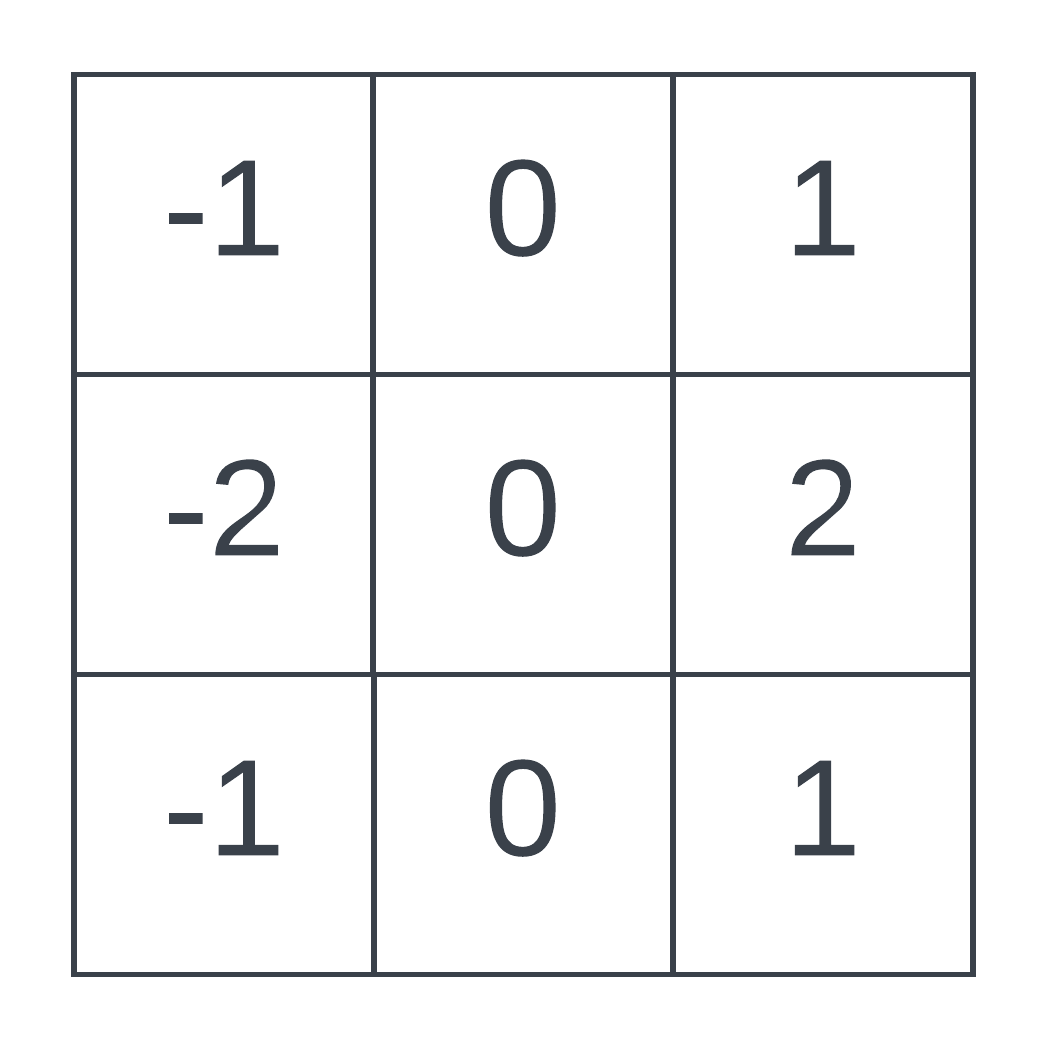
\includegraphics[width=0.2\linewidth]{Bilder/sobelfilter.png}
	\caption{Sobel-Filter (horizontal) mit vordefinierten Gewichtungen}
	\label{img:sobel}
\end{figure}
Ein Beispiel für einen gängigen Filterkern ist der horizontal angeordnete Sobel-Filter (\cite{kanopoulos_design_1988}) (Abbildung \ref{img:sobel}). Dieser wird verwendet, um horizontale Gradienten und Kanten in einem bestimmten Input zu detektieren. Der Filter berechnet bei jeder Position einen gewichteten Durchschnitt, womit im Laufe des Prozesses Kanten erkannt werden können. Dies ist der Fall, da die Gewichtungen des Filter so gewählt sind, dass diese besonders Empfindlich auf Veränderungen in horizontaler Richtung reagieren. Dadurch werden horizontale Kanten hervorgehoben, aber auch vertikale unterdrückt. Durch das Nutzen eines vertikalen Sobel-Filters ist das Verhalten umgekehrt. Nach Beenden des Durchgangs werden im Resultat -- einer Feature-Map -- die detektierten Kanten dargestellt.
\section{Angriffsmöglichkeiten auf Neuronale Netzwerke} \label{chpt:Stand_der_Technik_Angriffe}
Neuronale Netzwerke, obwohl leistungsfähig und vielseitig einsetzbar, eröffnen verschiedene Möglichkeiten für Angriffsvektoren, die von potenziellen Angreifern ausgenutzt werden können, um erheblichen Schaden anzurichten. Die Angriffe reichen von sogfältig konzipierten Manipulationen des Trainisngsprozesses bis hin zu raffinierten Methoden oder Modellinferenzen. Das ganze bringt  Konsequenzen für Entwickler und Unternehmen von Beeinträchtigung der KI-System-Verfügbarkeit bis hin zu gravierenden Datenschutzverletzungen von Involvierten mit sich.

Im Bereich der Bildklassifizierung hat sich ein gängiges Angriffsmuster in Form der sogenannten \glqq Adversarial Attacks\grqq{} etabliert. Bei dieser Art von Angriff zielt der Angreifer darauf ab, die Klassifizierungsergebnisse eines Modells zu manipulieren, indem er gezielt Störungen in den Eingabedaten einführt. Dies kann beispielsweise durch die Anwendung spezifischer Filter geschehen, die das Modell dazu verleiten, fehlerhafte Vorhersagen zu treffen. Diese Störungen sind häufig für das menschliche Auge kaum wahrnehmbar, führen jedoch zu erheblichen Beeinträchtigungen der Modellleistung bei der Verarbeitung von unvorhergesehenen, mit Störungen versehenen Daten. Adversarial Attacks gehören zu einer Gruppe von Angriffen, die darauf abzielen, die Genauigkeit von Modellen durch die Anwendung unterschiedlicher Techniken zu beeinträchtigen.

Zusätzlich zu Angriffen, die direkt auf die Modellvorhersagen abzielen, existieren auch solche, die die Qualität des Trainingsprozesses und die Gesamtleistung der Modelle beeinflussen. Ein Beispiel hierfür sind "Poisoning-Angriffe". Bei dieser Angriffsmethode werden absichtlich manipulierte Datenpunkte in Trainingsdatensätze eingeschleust, um die Qualität des Modelltrainings zu beeinträchtigen. Durch gezieltes Hinzufügen von verfälschten und missbrauchten Datenpunkten kann die Generalisierungsfähigkeit des Modells gegenüber neuen Daten erheblich beeinträchtigt werden.

Des Weiteren existieren diverse Angriffsmethoden, die darauf abzielen, die Modellintegrität und -sicherheit zu untergraben. Hierzu gehören "Transfer Attacks", bei denen Adversarial-Störungen von einem Modell auf ein anderes übertragen werden, um die Angriffseffektivität zu maximieren.

Eine weitere Angriffskategorie beschreiben die sogenannten Inferenz-Angriffe. Diese fokussieren sich auf den Versuch der Extraktion von Daten- und Modellparametern aus bereits trainierten neuronalen Netzwerken. Der Angreifer versucht durch gezielte Schwachstellenausnutzung und Analyse des Netzwerks beispielsweise herauszufinden, ob ein bestimmter Datenpunkt Teil des Trainingsdatensatzes war. Ein solcher Angriff wird als \glqq Membership-Inference-Angriff\grqq{} bezeichnet und wird in der Regel in Black-Box-Szenarien durchgeführt, in denen Modellparameter und genutzte Datensätze nicht bekannt sind. 

Die im Folgenden beschriebene Angriffsart der \glqq Modell-Inversionsangriffe\grqq{} gehört zu den Inferenz-Angriffen und bezeichnet eine Vorgehensweise, bei der Angreifer mittels gezielter Analyse von Modellausgaben im Rahmen unterschiedlicher Verfahren den Versuch unternehmen, Trainingsdaten zu rekonstruieren.

% Data Poisoning (Trainingsprozess)
% Inferenz Angriffe (Model Inverison, Model Extraction, Membership inferenz)
% Adversarial Attacks
\subsection{Modell-Inversionsangriffe} \label{subsec: MIAttack}
Bei Modell-Inversionsangriffen wird die Interaktion mit einem trainierten neuronalen Netzwerk genutzt, um Einblicke in den zugrunde liegenden Trainingsdatensatz zu gewinnen. Dies geschieht durch eine systematische Analyse der Ausgaben des Modells in Verbindung mit spezifischen Inversionsalgorithmen, die darauf abzielen, die Eingabedaten, die zu den beobachteten Modellausgaben geführt haben, zu rekonstruieren. Der Angreifer strebt dabei an, latente Merkmale und Muster der Trainingsdaten zu extrahieren, was nicht nur eine potenzielle Verletzung der Privatsphäre der in den Trainingsdatensatz eingeflossenen Informationen darstellen kann, sondern auch die Gefahr birgt, dass sensible oder persönliche Daten durch die Analyse des Modells exponiert werden.
\subsubsection{Angriffsziel}
Das Hauptziel von Modell-Inversionsangriffen besteht darin, interene Merkmale, Strukturen und Muster der im Training verwendeten Daten zu extrahieren, um eine mögliche Rekonstruktion auszuführen. Dabei geht man, gegensätzlich zu \glqq Adversarial Attacks\grqq{}, den Weg vom Ausgabebereich des Modells hin zum Eingabebereich, um damit Generierungen der Daten auszuführen. Dies geschieht auf Basis der gezielten Analyse der Ausgabe eines Modells bezüglich eines Inputs $I$. Neben den sichtlichen Merkmalen zielt diese Angriffsart auch auf die Rekonstruktion latenter Merkmale und Muster ab. Daneben kann man durch die Durchführung Informationen über die Art der Daten und verschiedene Muster im Training erlangen, um darauf auf die Reaktion bezüglich bestimmter Datenpunkte schließen zu können.

Durch die Extraktion latenter und visueller Merkmale der Daten kann bei Verwendung sensibler Daten eine Verletzung der Privatsphäre zustande kommen. Dabei können personenbezogene Informationen über Teilnehmende des Trainingsdatensatzes oder auch vertrauliche Merkmale der Daten exponiert werden.
\subsubsection{Angriffsvektoren}
Im Nachfolgenden werden potenzielle Angriffsvektoren beschrieben, die im Rahmen der Ausführung eines Angriffs genutzt werden, um optimale Ergebnisse zu erzielen.

Die einfachste Methode, die keine Informationen über verwendete Daten und interne Modellstrukturen erfordert, besteht in der Analyse der Modellausgabe im Hinblick auf bestimmte Eingabedaten. Dadurch können Angreifer Rückschlüsse auf innere Strukturen, Muster und Merkmale ziehen. Dies wird durch die Beobachtung von Wahrscheinlichkeiten oder Genauigkeiten der Modellausgabe auf der Grundlage bestimmter Eingaben $I$ erreicht.

Ein weiterer Angriffsvektor für die Durchführung wird durch interne Informationen des Modells dargestellt. Dies kann beispielsweiße durch die zugrunde liegenden Gradienten der Verlustfunktion geschehen. Dieser Gradienten-basierte Vektor ermöglicht dem Angreifer eine Approximation der Genauigkeit durch einen bestimmten Iterationsprozess basierend auf einen Input $I$. Dieses Verfahren erfordert oft Gradienteninformationen des Modells. 

In Black-Box Szenarien greift man auf den Vektor der Modellausgabe zurück. Hierbei versucht der Angreifer iterativ den Input $I$ zu verändern, sodass die Genauigkeit des Modells bezüglich der Zielklasse maximiert wird. 
\subsubsection{Verteidigungsstrategien}{\label{diff_privacy}}
Verteidigungsmaßnahmen gegenüber Modell-Inversionsangriffen sind von entscheidender Bedeutung, um die Privatsphäre und Sicherheit von neuronalen Netzwerken zu gewährleisten. Durch die Implementierung geeigneter Schutzmaßnahmen können potenzielle Angreifer daran gehindert werden, auf sensible Informationen der Trainingsdaten zuzugreifen und diese zu rekonstruieren.

Diese Verteidigungsmaßnahmen zielen darauf ab, die Effektivität von Modell-Inversionsangriffen bei nahezu gleichbleibender Modellleistung zu reduzieren und den Informationsverlust über Trainingsdaten zu minimieren. Dabei werden verschiedene Techniken eingesetzt, um den Rekonstruktionsprozess durch die Minimierung der Angriffsvektoren zu erschweren und den Angreifer von einer erfolgreichen Analyse der Modellausgaben abzuhalten.

Im Kapitel \ref{chpt:DefenseMI} dieser Arbeit werden konkrete Verteidigungsstrategien anderer Forschungsarbeiten gegenüber Modell-Inversionsangriffen eingehend beleuchtet, beschrieben und bewertet. Die strategischen Ansätze werden dabei darauf abzielen, sowohl die Ausgabewerte des Modells als auch interne Modellinformationen zu schützen, um die Extraktion sensibler Trainingsdaten zu vereiteln. Durch die Beschreibung detaillierter Untersuchungen dieser Verteidigungsstrategien wird eine umfassende Einsicht in bewährte Praktiken zur Abschwächung von Modell-Inversionsangriffen ermöglicht.

Die Ergebnisse der Implementierung von differentieller Privatsphäre, einer Verteidigungsmaßnahme, die durch Verhinderung von Overfitting und das Einfügen von Rauschen im Trainingsprozess auf eine geschütztere Modellentwicklung abzielt, sind in Kapitel \ref{chpt:dpnn_stats} beschrieben und dargestellt.



   \chapter{Stand der Technik} \label{chpt:Stand_der_Technik_Main}


%\section{Angriffsmöglichkeiten auf Neuronale Netzwerke} \label{chpt:Stand_der_Technik_Angriffe}
Neuronale Netzwerke, obwohl leistungsfähig und vielseitig einsetzbar, eröffnen verschiedene Möglichkeiten für Angriffsvektoren, die von potenziellen Angreifern ausgenutzt werden können, um erheblichen Schaden anzurichten. Die Angriffe reichen von sogfältig konzipierten Manipulationen des Trainisngsprozesses bis hin zu raffinierten Methoden oder Modellinferenzen. Das ganze bringt  Konsequenzen für Entwickler und Unternehmen von Beeinträchtigung der KI-System-Verfügbarkeit bis hin zu gravierenden Datenschutzverletzungen von Involvierten mit sich.

Im Bereich der Bildklassifizierung hat sich ein gängiges Angriffsmuster in Form der sogenannten \glqq Adversarial Attacks\grqq{} etabliert. Bei dieser Art von Angriff zielt der Angreifer darauf ab, die Klassifizierungsergebnisse eines Modells zu manipulieren, indem er gezielt Störungen in den Eingabedaten einführt. Dies kann beispielsweise durch die Anwendung spezifischer Filter geschehen, die das Modell dazu verleiten, fehlerhafte Vorhersagen zu treffen. Diese Störungen sind häufig für das menschliche Auge kaum wahrnehmbar, führen jedoch zu erheblichen Beeinträchtigungen der Modellleistung bei der Verarbeitung von unvorhergesehenen, mit Störungen versehenen Daten. Adversarial Attacks gehören zu einer Gruppe von Angriffen, die darauf abzielen, die Genauigkeit von Modellen durch die Anwendung unterschiedlicher Techniken zu beeinträchtigen.

Zusätzlich zu Angriffen, die direkt auf die Modellvorhersagen abzielen, existieren auch solche, die die Qualität des Trainingsprozesses und die Gesamtleistung der Modelle beeinflussen. Ein Beispiel hierfür sind "Poisoning-Angriffe". Bei dieser Angriffsmethode werden absichtlich manipulierte Datenpunkte in Trainingsdatensätze eingeschleust, um die Qualität des Modelltrainings zu beeinträchtigen. Durch gezieltes Hinzufügen von verfälschten und missbrauchten Datenpunkten kann die Generalisierungsfähigkeit des Modells gegenüber neuen Daten erheblich beeinträchtigt werden.

Des Weiteren existieren diverse Angriffsmethoden, die darauf abzielen, die Modellintegrität und -sicherheit zu untergraben. Hierzu gehören "Transfer Attacks", bei denen Adversarial-Störungen von einem Modell auf ein anderes übertragen werden, um die Angriffseffektivität zu maximieren.

Eine weitere Angriffskategorie beschreiben die sogenannten Inferenz-Angriffe. Diese fokussieren sich auf den Versuch der Extraktion von Daten- und Modellparametern aus bereits trainierten neuronalen Netzwerken. Der Angreifer versucht durch gezielte Schwachstellenausnutzung und Analyse des Netzwerks beispielsweise herauszufinden, ob ein bestimmter Datenpunkt Teil des Trainingsdatensatzes war. Ein solcher Angriff wird als \glqq Membership-Inference-Angriff\grqq{} bezeichnet und wird in der Regel in Black-Box-Szenarien durchgeführt, in denen Modellparameter und genutzte Datensätze nicht bekannt sind. 

Die im Folgenden beschriebene Angriffsart der \glqq Modell-Inversionsangriffe\grqq{} gehört zu den Inferenz-Angriffen und bezeichnet eine Vorgehensweise, bei der Angreifer mittels gezielter Analyse von Modellausgaben im Rahmen unterschiedlicher Verfahren den Versuch unternehmen, Trainingsdaten zu rekonstruieren.

% Data Poisoning (Trainingsprozess)
% Inferenz Angriffe (Model Inverison, Model Extraction, Membership inferenz)
% Adversarial Attacks
\subsection{Modell-Inversionsangriffe} \label{subsec: MIAttack}
Bei Modell-Inversionsangriffen wird die Interaktion mit einem trainierten neuronalen Netzwerk genutzt, um Einblicke in den zugrunde liegenden Trainingsdatensatz zu gewinnen. Dies geschieht durch eine systematische Analyse der Ausgaben des Modells in Verbindung mit spezifischen Inversionsalgorithmen, die darauf abzielen, die Eingabedaten, die zu den beobachteten Modellausgaben geführt haben, zu rekonstruieren. Der Angreifer strebt dabei an, latente Merkmale und Muster der Trainingsdaten zu extrahieren, was nicht nur eine potenzielle Verletzung der Privatsphäre der in den Trainingsdatensatz eingeflossenen Informationen darstellen kann, sondern auch die Gefahr birgt, dass sensible oder persönliche Daten durch die Analyse des Modells exponiert werden.
\subsubsection{Angriffsziel}
Das Hauptziel von Modell-Inversionsangriffen besteht darin, interene Merkmale, Strukturen und Muster der im Training verwendeten Daten zu extrahieren, um eine mögliche Rekonstruktion auszuführen. Dabei geht man, gegensätzlich zu \glqq Adversarial Attacks\grqq{}, den Weg vom Ausgabebereich des Modells hin zum Eingabebereich, um damit Generierungen der Daten auszuführen. Dies geschieht auf Basis der gezielten Analyse der Ausgabe eines Modells bezüglich eines Inputs $I$. Neben den sichtlichen Merkmalen zielt diese Angriffsart auch auf die Rekonstruktion latenter Merkmale und Muster ab. Daneben kann man durch die Durchführung Informationen über die Art der Daten und verschiedene Muster im Training erlangen, um darauf auf die Reaktion bezüglich bestimmter Datenpunkte schließen zu können.

Durch die Extraktion latenter und visueller Merkmale der Daten kann bei Verwendung sensibler Daten eine Verletzung der Privatsphäre zustande kommen. Dabei können personenbezogene Informationen über Teilnehmende des Trainingsdatensatzes oder auch vertrauliche Merkmale der Daten exponiert werden.
\subsubsection{Angriffsvektoren}
Im Nachfolgenden werden potenzielle Angriffsvektoren beschrieben, die im Rahmen der Ausführung eines Angriffs genutzt werden, um optimale Ergebnisse zu erzielen.

Die einfachste Methode, die keine Informationen über verwendete Daten und interne Modellstrukturen erfordert, besteht in der Analyse der Modellausgabe im Hinblick auf bestimmte Eingabedaten. Dadurch können Angreifer Rückschlüsse auf innere Strukturen, Muster und Merkmale ziehen. Dies wird durch die Beobachtung von Wahrscheinlichkeiten oder Genauigkeiten der Modellausgabe auf der Grundlage bestimmter Eingaben $I$ erreicht.

Ein weiterer Angriffsvektor für die Durchführung wird durch interne Informationen des Modells dargestellt. Dies kann beispielsweiße durch die zugrunde liegenden Gradienten der Verlustfunktion geschehen. Dieser Gradienten-basierte Vektor ermöglicht dem Angreifer eine Approximation der Genauigkeit durch einen bestimmten Iterationsprozess basierend auf einen Input $I$. Dieses Verfahren erfordert oft Gradienteninformationen des Modells. 

In Black-Box Szenarien greift man auf den Vektor der Modellausgabe zurück. Hierbei versucht der Angreifer iterativ den Input $I$ zu verändern, sodass die Genauigkeit des Modells bezüglich der Zielklasse maximiert wird. 
\subsubsection{Verteidigungsstrategien}{\label{diff_privacy}}
Verteidigungsmaßnahmen gegenüber Modell-Inversionsangriffen sind von entscheidender Bedeutung, um die Privatsphäre und Sicherheit von neuronalen Netzwerken zu gewährleisten. Durch die Implementierung geeigneter Schutzmaßnahmen können potenzielle Angreifer daran gehindert werden, auf sensible Informationen der Trainingsdaten zuzugreifen und diese zu rekonstruieren.

Diese Verteidigungsmaßnahmen zielen darauf ab, die Effektivität von Modell-Inversionsangriffen bei nahezu gleichbleibender Modellleistung zu reduzieren und den Informationsverlust über Trainingsdaten zu minimieren. Dabei werden verschiedene Techniken eingesetzt, um den Rekonstruktionsprozess durch die Minimierung der Angriffsvektoren zu erschweren und den Angreifer von einer erfolgreichen Analyse der Modellausgaben abzuhalten.

Im Kapitel \ref{chpt:DefenseMI} dieser Arbeit werden konkrete Verteidigungsstrategien anderer Forschungsarbeiten gegenüber Modell-Inversionsangriffen eingehend beleuchtet, beschrieben und bewertet. Die strategischen Ansätze werden dabei darauf abzielen, sowohl die Ausgabewerte des Modells als auch interne Modellinformationen zu schützen, um die Extraktion sensibler Trainingsdaten zu vereiteln. Durch die Beschreibung detaillierter Untersuchungen dieser Verteidigungsstrategien wird eine umfassende Einsicht in bewährte Praktiken zur Abschwächung von Modell-Inversionsangriffen ermöglicht.

Die Ergebnisse der Implementierung von differentieller Privatsphäre, einer Verteidigungsmaßnahme, die durch Verhinderung von Overfitting und das Einfügen von Rauschen im Trainingsprozess auf eine geschütztere Modellentwicklung abzielt, sind in Kapitel \ref{chpt:dpnn_stats} beschrieben und dargestellt.

\section{Modell-Inversions Angriffe} \label{chpt:Stand_der_Technik_MI}


   \chapter{Implementierung} \label{chpt:Implementierung_Main}

\section{Experimentelles Setup}
Das folgende Kapitel verdeutlicht den Aufbau der Experimentierumgebung, die für die technische Durchführung benötigt wurde. Dabei wird auf Datensätze, Modelle und deren Strukturen, wie auch auf die Implementierung von Angriffsmethoden und Verteidigungsmaßnahmen eingegangen. Die Auswahl und Konfiguration dieser Elemente sind entscheidend für die Reproduzierbarkeit der Experimente sowie für die Validität und Aussagekraft der ausgearbeiteten Ergebnisse.
\subsection{Datensätze}\label{subsection:datensaetze}
%mnist
%celeba
%ffhq
In diesem Abschnitt werden die Datensätze vorgestellt, die als Grundlage für die Trainings- und Angriffsdurchführungen in dieser Forschungsarbeit dienen. Eine sorgfältige Auswahl und detaillierte Beschreibung dieser Datensätze sind von zentraler Bedeutung, um die Integrität der Experimente zu gewährleisten und eine solide Grundlage für die Analyse der Ergebnisse und Beobachtungen zu schaffen.

In dieser Arbeit wurde aus Gründen der Einfachheit der MNIST-Datensatz (\cite{noauthor_mnist_nodate}) verwendet, welcher eine präzise Abfolge von Ziffern repräsentiert. Dieser Datensatz umfasst verschiedene Datenpunkte, die den Klassen der Zahlen 0 bis 9 zugeordnet sind. 

\begin{figure}[H]
	\centering
	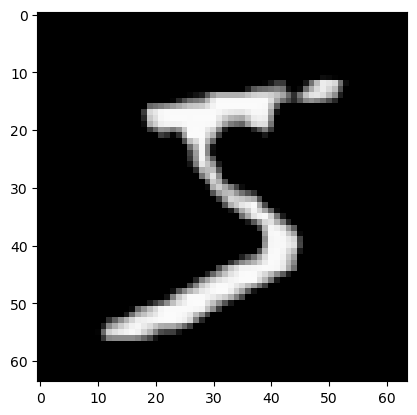
\includegraphics[width=0.2\linewidth]{Bilder/5_mnist.png}
	\caption{Beispielbild des MNIST-Datensatzes}
	\label{img:mnist}
\end{figure}

Die Datenpunkte sind in Form von sogenannten Ein-Kanal-Bildern repräsentiert, die vom menschlichen Auge in bestimmten Darstellungen als schwarz-weiß wahrgenommen werden (siehe Bild \ref{img:mnist}). Die Größe der Bilder, die zur Erstellung des Trainingsdatensatzes verwendet wurde, beträgt $64 \times 64$ Pixel. Dabei besitzt jeder Pixel einen normalisierten Wert zwischen 0 und 1, der die \glqq Farbe\grqq{} festlegt. Mit der Zusammensetzung aller Pixel entsteht das finale Bild.

Die Entscheidung für den MNIST-Datensatz wurde aufgrund seiner weiten Verbreitung in der Forschung und seiner klaren Struktur zur Repräsentation von Ziffern getroffen, wobei die Bildmerkmale vergleichsweise als \glqq einfach\grqq{} gelten. Die Fokussierung auf Zahlen im Bereich von 0 bis 9 ermöglicht eine gezielte Untersuchung spezifischer Klassen und vereinfacht die Interpretation der Ergebnisse. Dies erleichtert eine anschaulichere Analyse der durchgeführten Angriffe und liefert dem Betrachter klare und eindeutige Ergebnisse.

Der MNIST-Datensatz eignet sich besonders gut für die Evaluierung von Angriffen aufgrund seiner klaren Struktur und begrenzten Klassenanzahl. Dies ermöglicht eine präzise Bewertung der Wirksamkeit von Verteidigungsmaßnahmen und bietet gleichzeitig eine klare Vergleichsbasis für verschiedene Angriffsszenarien. Darüber hinaus hat sich gezeigt, dass auch komplexe Modelle wie das VGG16-Netzwerk auf Basis des MNIST-Datensatzes effizient trainiert werden können und bereits nach wenigen Epochen eine bemerkenswert hohe Genauigkeit auf Testdaten aufweisen.

Im Kontext neuronaler Netzwerke, die für die Generierung von Bildern eingesetzt werden, offenbart sich, dass diese rasch auf Grundlage des MNIST-Datensatzes angepasst werden können. Diese Modelle generieren zügig Bilder, die eine deutliche Ähnlichkeit zum Trainingsdatensatz aufweisen. Neben den zuvor erwähnten Gründen stellt die Veranschaulichung von Angriffen einen weiteren relevanten Aspekt für die Nutzung dieses Datensatzes dar. Aufgrund der als \glqq einfach\grqq{} geltenden Struktur der Bilder lässt sich zügig ein Vergleich zwischen Angriffen auf verschiedene Modelle herstellen, was die klare Veranschaulichung der Ergebnisse ermöglicht. Diese \glqq Einfachheit\grqq{} erweist sich als vorteilhaft für die transparente und effektive Analyse unterschiedlicher Angriffsstrategien sowie deren Auswirkungen auf die Bildgenerierung neuronaler Netzwerke.

Neben dem MNIST- wurde auch der CelebA-Datensatz (\cite{noauthor_celeba_nodate}) verwendet, der verschiedene Gesichtsbilder von 10.177 berühmten Personen in verschiedenen Klassen beinhaltet. Insgesamt hat er damit über 200.000 Bilder. Dieser eignet sich für verschiedene Use-Cases, wobei er in diesem Fall lediglich als Trainingsdatensatz für einen \glqq Personen\grqq-Klassifikator genutzt wurde. Auch hier werden die Bilder während des Ladens auf eine Größe von $64 \times 64$ Pixeln verändert und entstehen im Gegensatz zu den MNIST-Bildern aus 3 Kanälen. Auch hier wird jeder dieser Pixel auf einen normalisierten Wert zwischen 0 und 1 transformiert. Dabei wird jeweils rot, grün und blau von einem bestimmten Kanal repräsentiert. 

Der CelebA-Datensatz wurde als Vergleichsdatensatz zum zuvor genannten MNIST-Datensatz ausgewählt. Dies geschah sowohl, um Angriffe auf komplexere Datensätze zu prüfen, als auch, um Black-Box-Angriffe basierend auf einen bezüglich des CelebA-Datensatz trainierten Klassifizierer auf Grundlage eines anderen Gesichtsdatensatzes (\cite{noauthor_nvlabsffhq-dataset_2023}) zu erforschen. Diese Entscheidung ermöglichte die Simulation verschiedener Angriffsszenarien, die diverse Strategien und Durchführungsprozesse umfassen.

\begin{figure}[H]
	\centering
	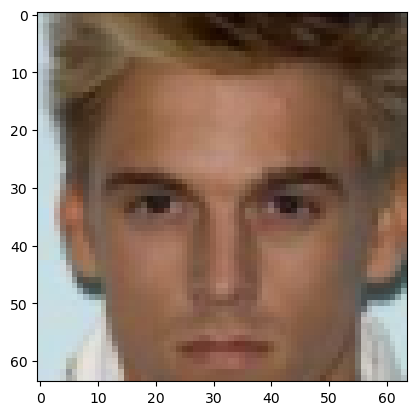
\includegraphics[width=0.2\linewidth]{Bilder/0_celeba_one.png}
	\caption{Beispielbild des CelebA-Datensatzes}
	\label{img:celeba}
\end{figure}

Die Auswahl des CelebA-Datensatzes ermöglichte eine erweiterte Untersuchung der Robustheit von Modellen gegenüber Angriffen, insbesondere auf dem Gebiet der Gesichtsbilderkennung. Die Verwendung von CelebA erlaubte nicht nur die Erweiterung des Anwendungsbereichs auf komplexere und realistischere Bilder, sondern ermöglichte auch eine generalisiertere Beurteilung der Sicherheitsmechanismen. Hierbei wurde der Fokus auf die Diversität von Gesichtsmerkmalen und -attributen gelegt, um die Widerstandsfähigkeit gegenüber unterschiedlichen Angriffsdurchführungen zu prüfen.

Die vielseitige Nutzung des CelebA-Datensatzes erstreckte sich über verschiedene Trainingsparadigmen. Einerseits wurde der Datensatz zur Schulung von Klassifikatoren herangezogen, die auf der VGG16-Architektur basierten. Andererseits wurde er auch für das Training eines herkömmlichen DCGAN-Netzwerks verwendet, um die Generierung von \glqq neuen\grqq{} Gesichtsbildern zu ermöglichen. Dies ermöglichte die Evaluierung der Anfälligkeit von Modellen unterschiedlicher Architekturen gegenüber Angriffen und trug zur Erweiterung des Verständnisses für die Sicherheit von Gesichtsdatensätzen bei.

Neben den Hauptdatensätzen CelebA und MNIST wurde der FFHQ-Datensatz (\cite{noauthor_nvlabsffhq-dataset_2023}) in dieser Arbeit integriert. Die \glqq rohen\grqq{} Bilddaten dieses Datensatzes weisen eine beeindruckende Größe von $1024 \times 1024$ auf und repräsentieren qualitativ hochwertige Bilder. Der FFHQ-Datensatz wurde eingeführt, um die Untersuchungen auf realistische Gesichtsbilder und einen unbekannten Datensatz zu erweitern. Hierbei wurde ein vortrainiertes Style-GAN Netzwerk auf Basis dieses Datensatzes verwendet, um realistische Gesichtsbilder zu generieren.

\begin{figure}[H]
	\centering
	
\includegraphics[width=0.4\linewidth]{Bilder/ffhq.png}
	\caption{Beispielbilder des Flickr-Faces-HQ-Datensatzes}
	\label{img:ffhq}
\end{figure}

Das Style-GAN Netzwerk, basierend auf dem FFHQ-Datensatz, ermöglichte nicht nur die Erstellung von hochqualitativen Gesichtsbildern, sondern trug auch zur Erweiterung der Vielfalt in den untersuchten Merkmalen bei. Im Gegensatz zu CelebA bietet der FFHQ-Datensatz eine breitere Auswahl an Herkunft, Altersgruppen und anderen charakteristischen Merkmalen.

Die Integration des FFHQ-Datensatzes eröffnete die Möglichkeit, reale Bildqualität in die Evaluierung von Angriffsszenarien einzubeziehen. Die repräsentativen Bilder des FFHQ-Datensatzes förderten die präzise Analyse von Angriffen auf hochauflösende Gesichtsbilder und trugen zur Entwicklung eines umfassenderen Verständnisses der Sicherheit von Gesichtsdatensätzen bei.
\subsection{Modelle}
%VGG16
%DCGAN
%StyleGAN
Die \textit{Architektur} der eingesetzten Modelle spielt eine zentrale Rolle in der Experimentierumgebung. Hier werden die gewählten Modelle hinsichtlich ihrer Struktur und Hyperparameter, die während des Traininsprozesses verwendet wurde, detailliert beschrieben. Eine genaue Vorstellung der Modelle ist entscheidend, um nachvollziehen zu können, wie diese auf die Datensätze angewendet wurden und welche Rolle sie in den folgenden Angriffs- und Verteidigungsszenarien spielen.

Die essentielle Architektur, die als Grundlage für den Klassifizierer dient, ist das VGG-16 Netzwerk (\cite{simonyan_very_2015}), ein CNN, das in der Bilderkennung eingesetzt wird. Dieses Netzwerk folgt dem Prinzip der \glqq Very Deep Convolutional Networks\grqq{} und zeichnet sich durch herausragende Merkmalsextraktionseigenschaften aus, wodurch es besonders für Bildklassifikationsaufgaben geeignet ist. Die Struktur setzt sich durch die sequenzielle Anordnung verschiedener Schichten zusammen, darunter Fully-Connected-, Pooling- und Convolutional-Schichten.
Das VGG-16 Netzwerk besteht insgesamt aus 16 Schichten, von denen 13 Convolutional- und 3 Fully-Connected-Schichten sind. Diese Schichten ermöglichen eine tiefgehende und hierarchische Repräsentation von Merkmalen, beginnend mit einfachen lokalen Strukturen bis hin zu abstrakteren und komplexeren Konzepten im Verlauf der Schichtfolge. Hervorzuheben ist, dass die Convolutional-Schichten Filter mit einer Größe von 3x3 Pixeln und einer Schrittweite von 1 Pixel verwenden, die Max-Pooling-Schichten eine Größe von 2x2 Pixeln und eine Schrittweite von 2 Pixeln aufweisen, und die Aktivierungsfunktion in allen Schichten, bis auf die finale Klassifikationsschicht, die ReLU-Funktion ist. Während des Vorwärtsdurchlaufs eines bestimmten Datenpunkts sind die Convolutional-Schichten maßgeblich für die Extraktion von Merkmalen verantwortlich.
Die Integration der vollvermaschten Schichten im Netzwerk fügt extrahierte Merkmale zusammen, um diese in der abschließenden Schicht des Bildklassifikators interpretieren zu können. Das Resultat ist ein Vektor, dessen Länge der Anzahl der Klassen im Datensatz entspricht, und der durch die Softmax-Aktivierungsfunktion erzeugt wird. Die Klassifikation erfolgt auf Basis eines personalisierten Headers, der eine vollvermaschte Schicht mit einer Softmax Aktivierungsfunktion als abschließende Schicht enthält. Die Neuronenanzahl dieser Schicht gleicht der Anzahl der Klassen im Datensatz.
Besondere Bedeutung kommt der Integration von Max-Pooling-Schichten in bestimmten Abschnitten des Netzwerks zu. Diese Schichten reduzieren die Merkmalskartengröße und erhöhen die Invarianz gegenüber kleinen Translationen im Eingabebild. Diese Struktur trägt dazu bei, die Robustheit des Modells zu steigern und seine Fähigkeit zur Erfassung invarianten Wissens zu stärken.
Hervorzuheben ist, dass das VGG-16 Netzwerk auf dem ImageNet-Datensatz trainiert wurde, der 1000 verschiedene Klassen von Objekten enthält. Die hohe Genauigkeit bei der Klassifizierung von Bildern macht es zu einem oft verwendeten vortrainierten Modell in verschiedenen Computer-Vision-Anwendungen. 

\textit{Anwendung} fand das neuronale Netzwerk, das auf der VGG-16 Netzarchitektur aufbaut, in zwei Klassifikationsmodellen, welche auf der einen Seite handgeschriebene Ziffern und auf der anderen Seite berühmte Gesichter klassifizieren sollen. Trainiert wurde hierbei auf Basis der in \ref{subsection:datensaetze} beschriebenen MNIST- und CelebA-Datensätze.


%% muss noch überarbeitet werden
\begin{table}[h]
	\centering
	\renewcommand{\arraystretch}{1.5}
	\resizebox{\textwidth}{!}{
		\begin{tabular}{c|ccccc|c}
			\textbf{Datensatz} & \textbf{Lernrate} & \textbf{Epochenanzahl} & \textbf{Batch-Größe} & \textbf{Momentum} & \textbf{Weight-Decay} & \textbf{Genauigkeit bezüglich Testdaten}\\
			\hline
			\textit{CelebA} & 1e-3 & 40 & 128 & 0.9 & 1e-4 & \textbf{99,6\%}\\
			\hline
			\textit{MNIST} & 1e-3 & 8 & 64 & 0.9 & 1e-4 & \textbf{99,6\%}\\
			\hline
		\end{tabular}
	}
	\caption{Hyperparameter des \glqq normalen\grqq{} Trainings bezüglich der angegebenen Datensätze}
	\label{tab:nn_train}
\end{table}

% Trainingsteil des VGG hinzufügen 
Hier soll erstmal blabla über Training eines VGG16 Netzwerks gemacht werden (wie es bei mir war).

Zur Durchführung der im vorliegenden Kontext beschriebenen Modell-Inversions-Angriffe ist ein neuronales Netzwerk erforderlich, das die Fähigkeit besitzt, spezifische Bilder zu generieren. In diesem Zusammenhang wurde das Deep Convolutional Generative Adversarial Network (DCGAN) gemäß der Arbeit von Radford et al. (\cite{radford_unsupervised_2016}) eingesetzt. Dieses Netzwerk zeichnet sich durch eine Vielzahl von speziellen architektonischen Merkmalen aus. Es besteht primär aus zwei Hauptkomponenten: dem Generator, der die Generierung neuer Datenpunkte durch zufälliges Rauschen übernimmt, und dem Diskriminator, der versucht, zwischen realen und gefälschten Bildern zu differenzieren.

Ein zentraler Aspekt dieser Architektur ist die tiefe Faltungsstruktur, die sowohl im Generator als auch im Diskriminator Verwendung findet. Diese Struktur ermöglicht die Erfassung räumlicher Strukturen in den generierten Daten. Im Gegensatz zu herkömmlichen Convolutional Neural Networks (CNNs) werden in der Architektur von DCGANs keine Pooling-Schichten verwendet, um Unschärfe zu vermeiden. Stattdessen setzt man auf Normalisierungsschichten, um das Training stabil zu gestalten und die Konvergenz der Verlustfunktionen zu beschleunigen.

Eine weitere Abweichung von konventionellen CNNs besteht in der Verwendung der LeakyReLU-Aktivierungsfunktion anstelle der üblichen ReLU-Funktion. Die LeakyReLU-Funktion lautet:
\[
\text{LeakyReLU}(x) = \begin{cases}
	x, & \text{if } x > 0 \\
	\alpha x, & \text{otherwise}
\end{cases}
\]
Hier repräsentiert $\alpha$ eine kleine, positive Konstante. Der Einsatz dieser modifizierten Aktivierungsfunktion zielt darauf ab, das Problem der \glqq tötenden Neuronen\grqq{} zu umgehen, das bei der Verwendung der ReLU-Aktivierungsfunktion auftreten kann. Dabei werden Neuronen während des Trainings inaktiv und tragen somit nicht zur Leistungssteigerung des Modells bei, sondern verschlechtern diese sogar.

Die Trainingseffizienz des DCGAN kann variieren, abhängig von der verwendeten Hardware. Es wird empfohlen, das Netzwerk auf einer oder mehreren GPUs zu trainieren, da diese leistungsfähiger sind als eine ausschließliche Verwendung der CPU. Eine alternative Möglichkeit besteht im Transfer Learning, bei dem ein bereits trainiertes Modell als Ausgangspunkt für das aktuelle Training dient. Allgemein lässt sich feststellen, dass mit zunehmenden Epochen eine Verbesserung der Qualität der neu generierten Bilder erkennbar ist.

%% muss noch überarbeitet werden
\begin{table}[h]
	\centering
	\renewcommand{\arraystretch}{1.5}
	\resizebox{\textwidth}{!}{
		\begin{tabular}{c|ccccc}
			\textbf{Datensatz} & \textbf{Lernrate} & \textbf{Epochenanzahl} & \textbf{Batch-Größe} & \textbf{Momentum} & \textbf{Weight-Decay}\\
			\hline
			\textit{CelebA} & 1e-3 & 40 & 128 & 0.9 & 1e-4\\
			\hline
			\textit{MNIST} & 1e-3 & 8 & 64 & 0.9 & 1e-4 \\
			\hline
		\end{tabular}
	}
	\caption{Hyperparameter eines DCGAN-Trainings bezüglich der angegebenen Datensätze}
	\label{tab:dcgan}
\end{table}

% Trainingsteil des DCGAN hinzufügen 
Hier soll erstmal blabla über Training eines DCGAN Netzwerks gemacht werden (wie es bei mir war).

Um die Angriffsszenarien erweitern zu können, wurde ein weiteres generatives Modell zur Erzeugung hochauflösender Gesichtsbilder verwendet. Dieses StyleGAN (\cite{karras_style-based_2019}) basiert auf dem Konzept der generativen adverariellen Netzwerke und umfass -- wie ein DCGAN -- sowohl Generator und Diskriminator. Hierbei generiert der Generator die neuen Bilder, die dann vom Diskriminator nach Qualität bewertet werden. Während des Trainings werden beide Komponenten verbessert, was qualitativ hochwertigere und realistischere Bilder mit sich bringt. Die StyleGAN-Architektur hat neben den realistischen Bildausgaben die Besonderheit, dass Stilvarationen in Generierungen gut zu kontrollieren sind. Dies bedeutet, dass bestimmte Merkmale, wie beispielsweise Mimik und Haarfarbe, separat manipuliert werden können, um dadurch individuelle Ergebnisse zu erzielen. Diese Art des GANs wurde nicht selbst trainiert, sondern vortrainiert von NVIDIA geladen.

Die Auswahl der genutzten Modelle, nämlich das VGG-16 Netzwerk, das Deep Convolutional Generative Adversarial Network (DCGAN) und das StyleGAN, erfolgte aufgrund ihrer spezifischen Eigenschaften und Anwendungsbereiche, die im Kontext der Experimente von entscheidender Bedeutung waren.

Das VGG-16 Netzwerk wurde als essenzielle Architektur für den Klassifizierer gewählt. Dieses Convolutional Neural Network (CNN) ist aufgrund seiner \glqq Very Deep Convolutional Networks\grqq-Struktur besonders geeignet für Bildklassifikationsaufgaben. Mit insgesamt 16 Schichten, darunter Convolutional-, Pooling- und Fully-Connected-Schichten, ermöglicht das VGG-16 Netzwerk eine tiefgehende und hierarchische Repräsentation von Merkmalen. Die Verwendung von 3x3 Pixel großen Filtern in den Convolutional-Schichten, 2x2 Pixel großen Max-Pooling-Schichten und der ReLU-Aktivierungsfunktion trägt zur Merkmalsextraktion und Robustheit des Modells bei. Die Integration von Max-Pooling-Schichten in bestimmten Abschnitten des Netzwerks unterstützt die Reduzierung der Merkmalskartengröße und erhöht die Invarianz gegenüber kleinen Translationen im Eingabebild. Das VGG-16 Netzwerk wurde auf dem ImageNet-Datensatz trainiert, was seine hohe Genauigkeit bei der Klassifizierung von Bildern erklärt. Diese Merkmale machten es zu einem geeigneten Modell für die Klassifikation von handgeschriebenen Ziffern und berühmten Gesichtern in den durchgeführten Experimenten.

Für die Durchführung von Modell-Inversions-Angriffen wurde das DCGAN ausgewählt. Die Entscheidung basierte auf seiner Fähigkeit, spezifische Bilder zu generieren, insbesondere im Kontext der Modell-Inversion. Die tiefe Faltungsarchitektur des DCGAN, ohne Pooling-Schichten, sondern mit Normalisierungsschichten, ermöglichte die Erfassung räumlicher Strukturen in den generierten Daten. Die Verwendung der LeakyReLU-Aktivierungsfunktion half, das Problem der "tötenden Neuronen" zu umgehen, und trug zur Verbesserung der Trainingseffizienz bei. Die Anpassung an unterschiedliche Hardware, einschließlich der Möglichkeit des Trainings auf GPUs und des Einsatzes von Transfer Learning, machte das DCGAN zu einem flexiblen Modell für die Experimente. Für die Szenarioerweiterung auf ungesehene Daten wurde das StyleGAN verwendet. Dieses GAN basiert auf dem generativen adversariellen Netzwerk-Konzept und ermöglicht die Kontrolle von Stilvariationen in den Generierungen. Die spezielle Fähigkeit, bestimmte Merkmale separat zu manipulieren, machte StyleGAN besonders geeignet für die Erzeugung realistischer und individualisierter Gesichtsbilder. Das Modell wurde nicht selbst trainiert, sondern vortrainiert von NVIDIA geladen, um qualitativ hochwertige Ergebnisse zu gewährleisten.

Insgesamt wurden die Modelle entsprechend ihrer Architektur, Trainingsdaten und Anwendungsbereiche ausgewählt, um die Experimente zu unterstützen und eine präzise Analyse der Angriffsszenarien und Verteidigungsstrategien zu ermöglichen.
\subsection{Angriffsmethoden}
%KEDMI
%RBMI
Dieser Abschnitt beleuchtet die implementierten Angriffsmethoden, die darauf abzielen, die Integrität und Sicherheit der Modelle zu kompromittieren. Die Wahl der Angriffsvektoren, deren Ausführung und Auswirkungen werden systematisch erläutert. Zusätzlich werden mögliche Schwächen der Modelle aufgezeigt, die durch die Angriffsmethoden ausgenutzt wurden. Die detaillierte Beschreibung ermöglicht es, die Reproduzierbarkeit der Angriffe zu gewährleisten und die Robustheit der Modelle zu bewerten. Der Angreifer nutzt das Wissen über en Trainingsdatensatz und die Modellparameter, um das Modell zu invertieren und ursprüngliche Trainings-Datenpunkte zu rekonstruieren. Hierbei finden verschiedene Verfahren für die Rekonstuktion, wie beispielsweise Regularisierung oder Gradientenabstiegsverfahren, Verwendung.

Der \glqq KEDMI\grqq-Angriff, wie in der Arbeit von Chen et al. (\cite{chen_knowledge-enriched_2021}) beschrieben, repräsentiert eine der beiden Angriffsmethoden, die für die durchgeführten Experimente von Relevanz waren. In diesem Kontext wird das Bestreben verfolgt, sensible Informationen aus einem bereits trainierten maschinellen Lernmodell zu rekonstruieren, indem das interne Wissen und die Struktur des Modells gezielt ausgenutzt werden. Durch die Anwendung des bekannten Modellwissens und die Implementierung des Konzepts der \glqq Wissensanreicherung\grqq, bei dem zusätzliche Informationen des Modells erfasst werden, handelt es sich um einen \glqq WhiteBox-basierten\grqq{} Angriff. Hierbei hat der Angreifer uneingeschränkten Zugriff auf die internen Funktionsweisen des Modells, einschließlich der Parameter, Architektur sowie der internen Darstellungen, und auf den genutzten Datensatz. Die Wissensanreicherung zielt darauf ab, Merkmale oder andere interne Repräsentationen des Modells zu extrahieren.

\begin{figure}[H]
	\centering
	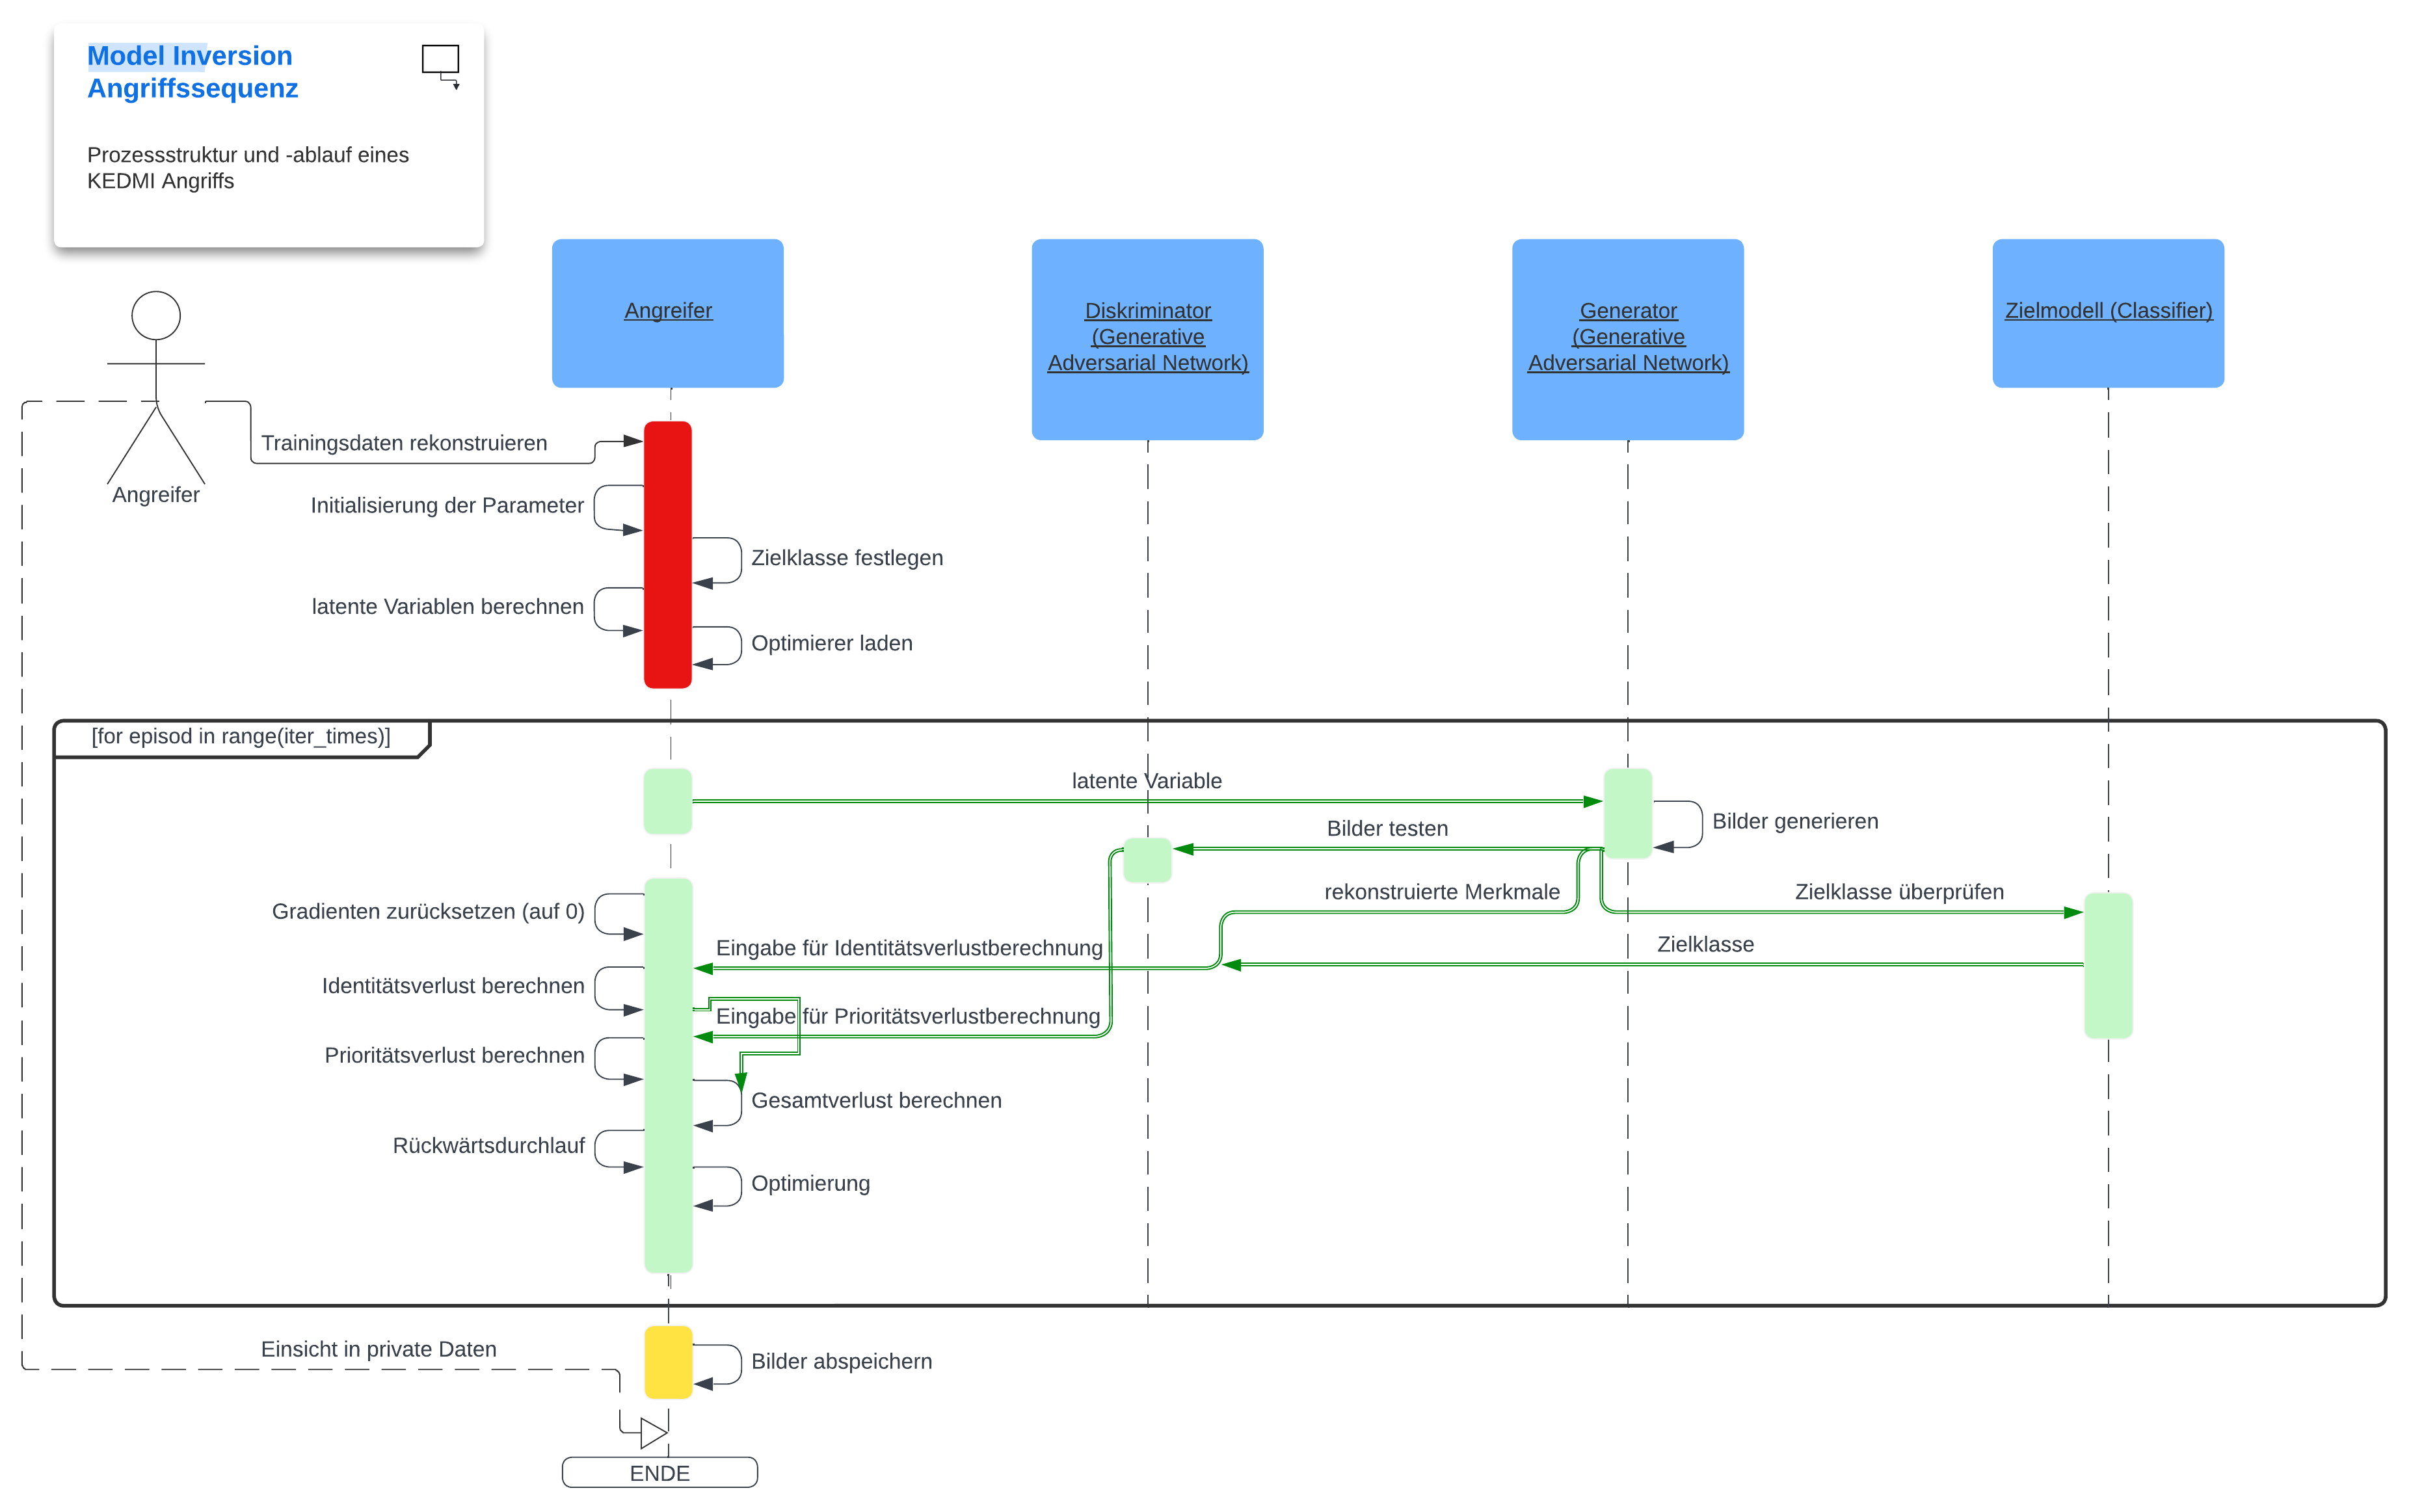
\includegraphics[width=1\linewidth]{Bilder/KEDMI_PROCESS.png}
	\caption{Prozessablauf eines KEDMI-Angriffs}
	\label{img:kedmi_process}
\end{figure}

Des Weiteren wurde eine Modellinversionsmethode angewandt, die auf dem Prinzip des bestärkenden Lernens basiert. Bei dieser Methode werden Konfidenzwerte oder -vektoren der generierten Bilder verwendet, um einem Agenten Belohnungen zuzuführen. Der Agent nutzt diese Belohnungen, um private Daten zu rekonstruieren, die während des Trainingsprozesses des Modells verwendet wurden. Aufgrund der begrenzten Zugriffsmöglichkeiten auf das Modell, bei dem der Zugriff auf die Konfidenzwertausgabe des Modells eingeschränkt ist, handelt es sich hierbei um einen sogenannten BlackBox-Angriff.
Der Ansatz des bestärkenden Lernens beinhaltet die Verwendung von Konfidenzwerten, die die Zuversicht oder Sicherheit des Modells in Bezug auf die generierten Daten repräsentieren. Diese Konfidenzwerte dienen als Belohnungen für den Agenten, der daraufhin die Aufgabe hat, die privaten Daten so zu rekonstruieren, dass die Belohnungen maximiert werden.

\begin{figure}[H]
	\centering
	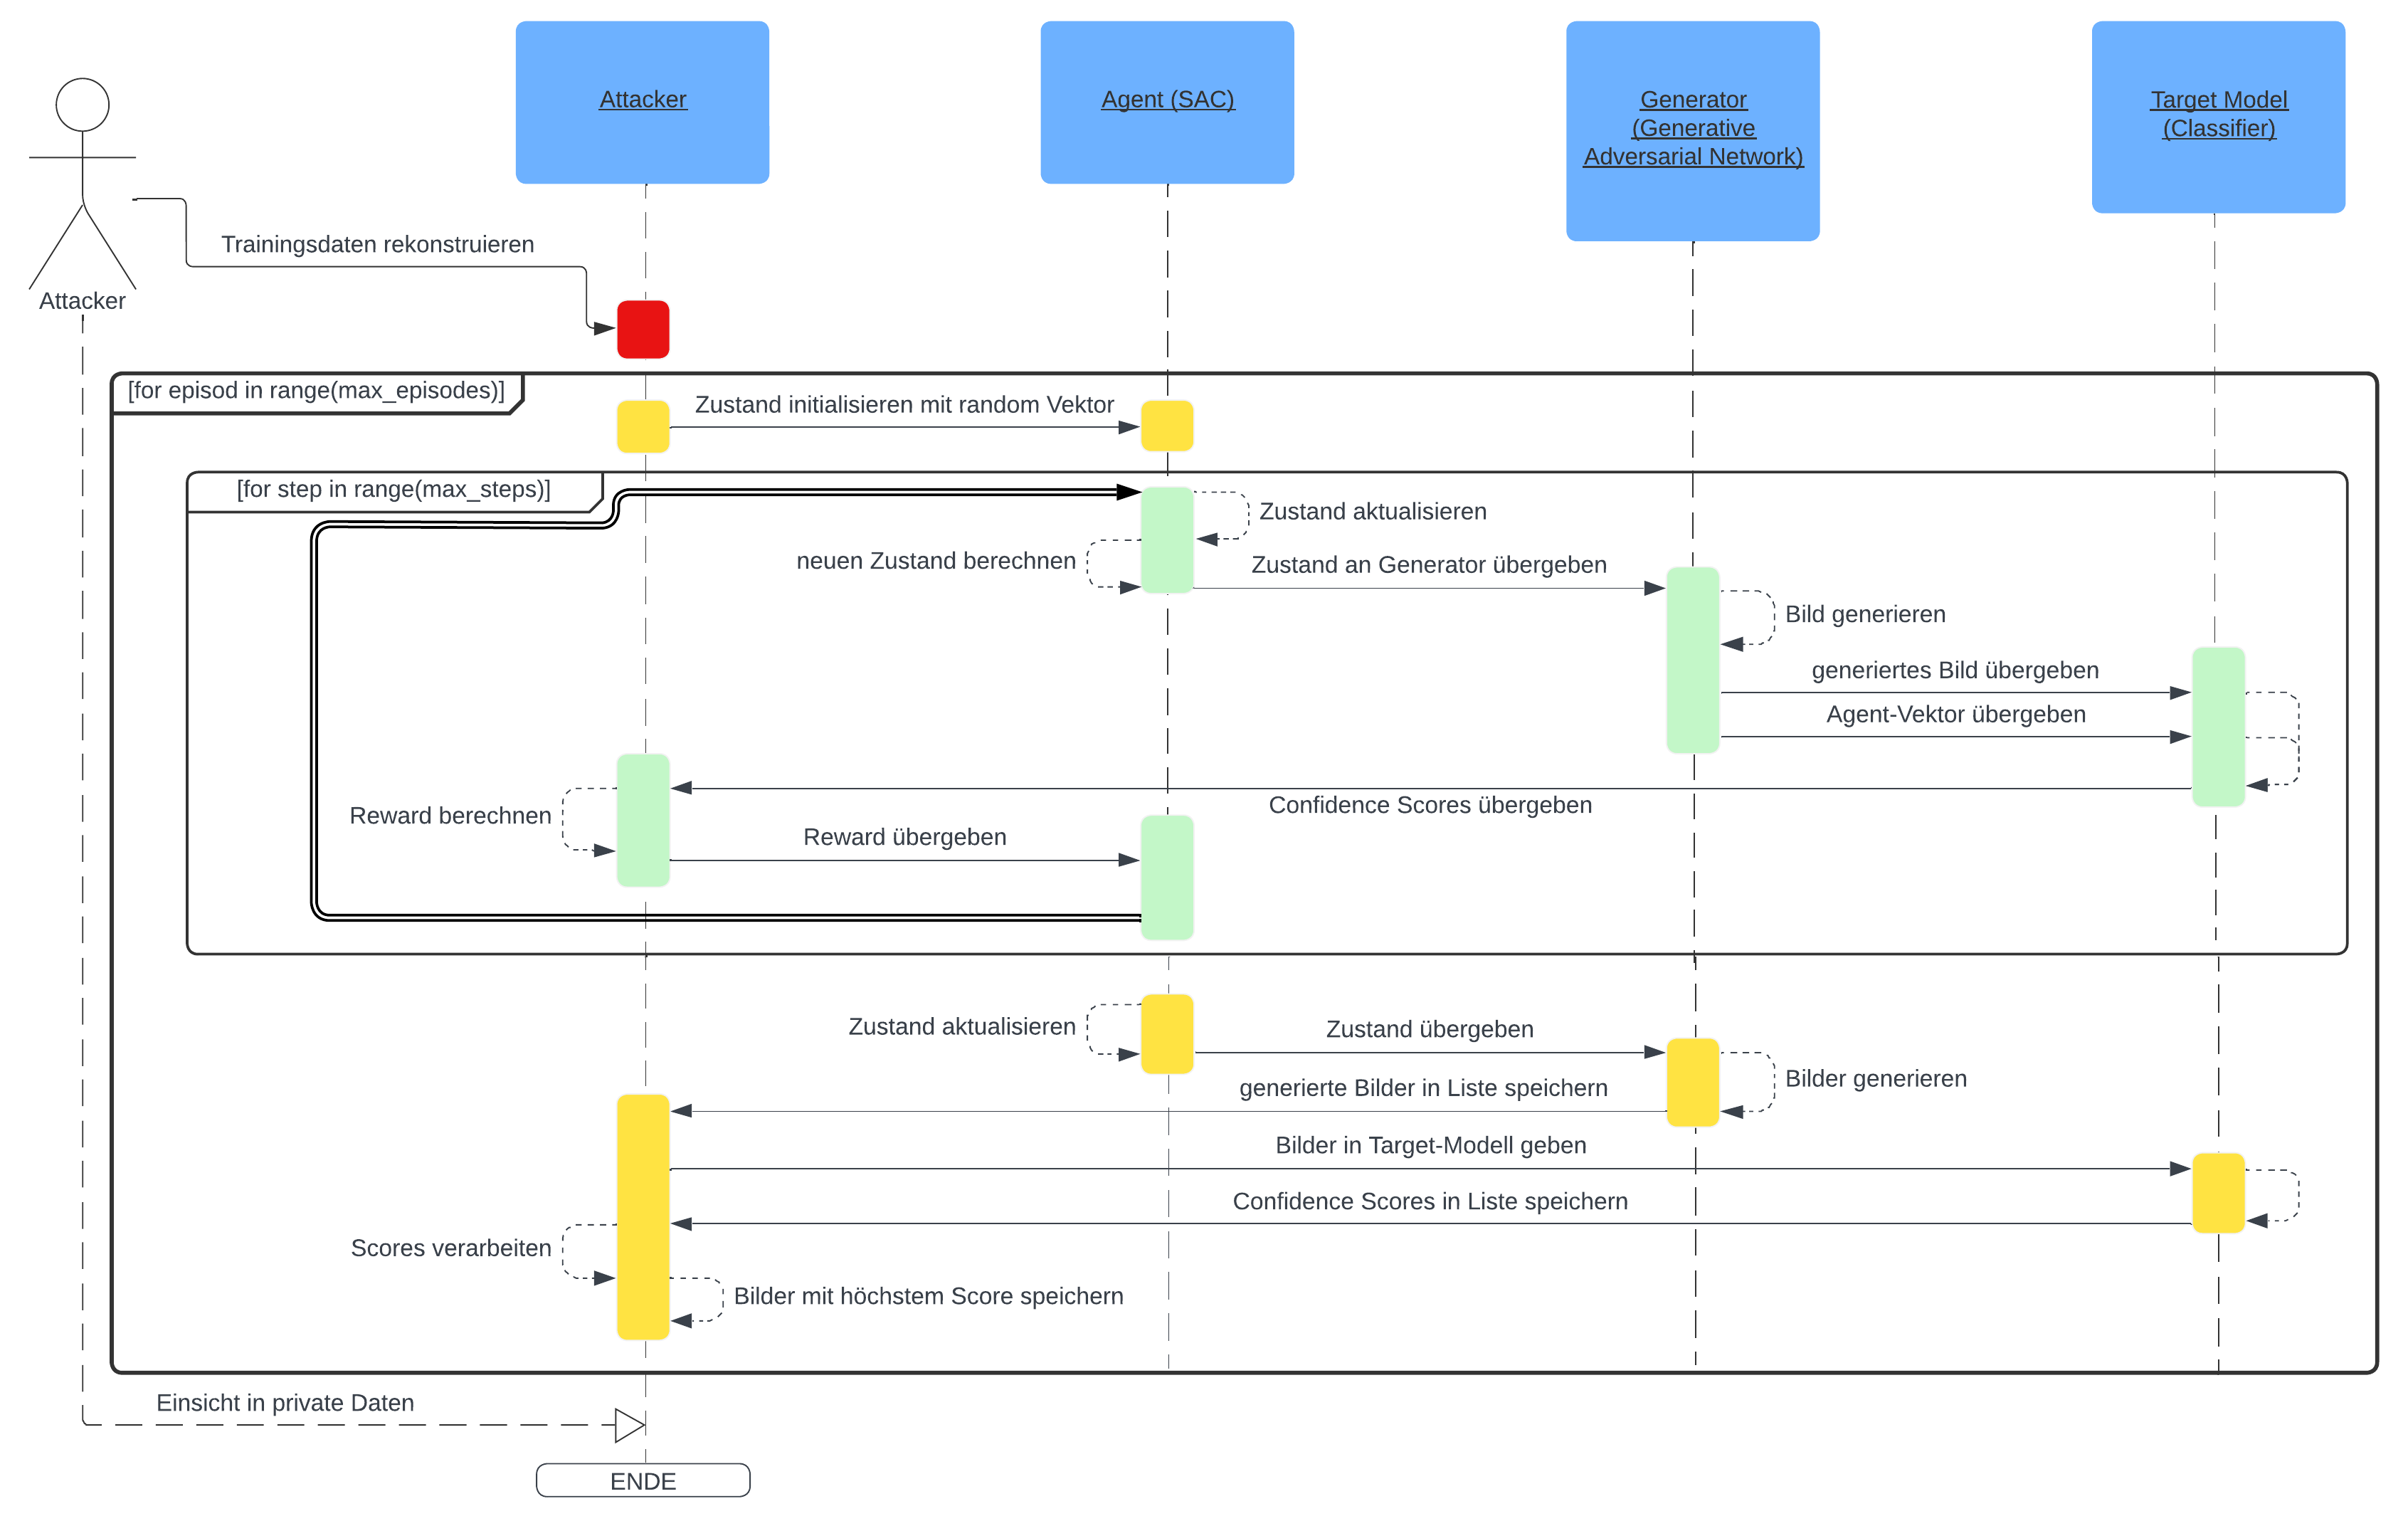
\includegraphics[width=1\linewidth]{Bilder/RBMI_PROCESS.png}
	\caption{Prozessablauf eines RBMI-Angriffs}
	\label{img:rbmi_process}
\end{figure}

Dieser Ansatz stellt eine besondere Herausforderung dar, da der Angreifer aufgrund der begrenzten Kenntnis über die internen Strukturen und Parameter des Modells alternative Methoden finden muss, um an sensible Informationen zu gelangen. In diesem Szenario wird bestärkendes Lernen als Mechanismus genutzt, um den Agenten dazu zu bringen, die unsichtbaren Merkmale der generierten Daten zu erlernen und somit private Informationen zu rekonstruieren.
\subsection{Verteidigungsmaßnahmen}
%Differential Privacy
Um den experimentellen Rahmen abzurunden, werden in diesem Abschnitt die implementierten Verteidigungsmaßnahmen präsentiert. Dies beinhaltet Schutzmechanismen, die darauf abzielen, Modelle gegen Angriffe zu stärken und ihre Robustheit zu verbessern. Die Wirksamkeit dieser Verteidigungsstrategien wird kritisch betrachtet, und es werden etwaige Limitationen oder Trade-offs diskutiert.

Für dieses Vorhaben wurde die Methode der differentiellen Privatsphäre, wie in Abschnitt \ref{diff_privacy} beschrieben, eingebunden. Diese Methode zielt darauf ab, Überanpassung (Overfitting) durch das Einbringen von Rauschen in die Trainingsdaten zu verhindern und die erfolgreiche Durchführung von Inferenzangriffen zu erschweren. Die Integration erfolgt mittels des sogenannten Opacus-Frameworks (\cite{noauthor_opacus_nodate}), welches die direkte Implementierung von Trainingsroutinen auf Basis von mit PyTorch erstellten Modellen ermöglicht.

\begin{figure}[H]
	\centering
	\hspace{-1.5cm}
	\includegraphics[width=0.9\linewidth]{Bilder/dpsgd.png}
	\caption{Trainingsprozess eines mit differentieller Privatsphäre durchgeführten Trainings}
	\label{img:dpsgd}
\end{figure}

Im Bild \ref{img:dpsgd} wird eine oberflächliche Visualisierung der Trainingsroutine eines neuronalen Netzwerks gezeigt, das auf Basis differentieller Privatsphäre trainiert wird. Dabei wird hervorgehoben, dass sich der Trainingsprozess von dem des \glqq normalen\grqq{} Trainings in verschiedenen Abschnitten durch spezifische Erweiterungen unterscheidet. Diese zusätzlichen Werte repräsentieren allesamt einen besonderen Mehrwert in den zusätzlichen Phasen des DP-SGD-Algorithmus (\cite[3]{abadi_deep_2016}).

Der \textit{Ablauf} des Algorithmus beginnt mit der Initialisierung verschiedener Parameter, die die Rahmenbedingungen des Trainings festlegen. Dazu zählen neben Hyperparametern wie der Lernrate $\eta_t$, dem Sensitivitätswert $S$, der Gruppierungs- und Rauschgröße ($L$ und $\sigma$), der Gradientenobergrenze $C$ auch Verlustfunktion 
\begin{equation}
	\mathcal{L}(\theta) = \frac{1}{N} \sum_{i=1} \mathcal{L}(\theta,x_i)
\end{equation}
sowie die Menge der Trainingsdaten $X$ bestehend aus Datenpunkten \{$x_1, x_2, \dots x_n$\}. Auf Basis dieser Werte folgt anschließend eine Schleife über eine bestimmte Epochenanzahl, die auch durch den Trainierenden festgelegt werden muss. In dieser Schleife führt man eine weitere aus, die zufällig über jeden Datenpunkt $x$ iteriert, um auf Basis des Werts verschiedene Operationen auszuführen. Zuerst wird der Gradient auf Basis der angegebenen Verlustfunktion und den aktuellen Modellparametern berechnet: 
\begin{equation}
	g_t(x_i) \leftarrow \nabla_{\theta_t} L(\theta_t, x_i)
\end{equation}
Durch die Berechnung eines Gradienten für jeden einzelnen Datenpunkt kann das Modell auf die spezifischen Eigenschaften angepasst und eine bessere Modellleistung herbeigeführt werden. Im folgenden Schritt wird auf Basis der übergebenen Gradientenobergrenze $C$ der zuvor erechnete Wert angepasst. Das sogenannte \glqq Gradienten-Clipping\grqq{} beschränkt den Datenpunkt der einzelnen Gradienten auf eine bestimmte Größe $C$: 
\begin{equation} 
	g_t(x_i) \leftarrow \frac{g_t(x_i)}{\max \left(1, \frac{\|g_t(x_i)\|_2}{C}\right)}
\end{equation}
Dadurch wird das Problem der explodierenden Gradienten (eng.: Gradient Explosion), das die Leistung und Qualität des Trainings stark beeinflusst, verhindert. Wenn der Wert von $g_t(x_i)$ den Wert $C$ übersteigt, wird dieser durch den Faktor der genannten Formel dividiert. Ein weiterer Vorteil ist dabei die Beschränkung der Sensitivität bezüglich einzelner Datenpunkte, die durch die Oberschwelle $C$ gesteuert werden kann. Je höher diese, desto größer ist das Rauschen, das in folgenden Schritten hinzugefügt werden muss, um den Schutz der Privatsphäre gewährleisten zu können.
Nachdem die Gradienten an das vorgegebene Intervall angepasst wurden, erfolgt die Zugabe von Rauschen zu den Datenpunkten auf Grundlage dieser Formel:
\begin{equation}
	\tilde{g}_t \leftarrow \frac{1}{L} \left( \sum_i \bar{g}_t(x_i) + N(0, \sigma^2C^2I) \right)
\end{equation}
Dabei wird jedem Datenpunkt für den bereits \glqq geclippten\grqq{} Gradienten ein Rauschterm hinzugefügt. Dieser wird durch die Normalverteilung mit Mittelwert 0 und einer Kovarianzmatrix $\Sigma = \sigma^2C^2I $ berechnet. $\sigma$ steht hierbei für die Standardabweichung des Rauschens und $C$ für die Obergrenze des Clippings. Durch das Hinzufügen des Rauschens versucht man die Sensitivität der einzelnen Datenpunkte zu verschleiern und den verstärkten Einfluss bestimmter Parameter auf die Aktualisierung der Modellparameter zu verhindern. Dies hat den Schutz der Privatsphäre zur Folge.

Nach Abschluss sämtlicher Berechnungen für eine festgelegte Anzahl von Datenpunkten, welche durch die Gruppierungsgröße $L$ definiert ist, werden diese zu einem sogenannten Mini-Batch zusammengeführt. Auf Grundlage dieses Mini-Batches erfolgt dann eine Aktualisierung der Modellparameter.

Die Anwendung dieses beschriebenen Prozesses dient dem Schutz der Privatsphäre der während des Trainings verwendeten Datenpunkte. Das wird durch die Vermeidung eines zu großen Einflusses spezifischer Datenpunkte während der Aktualisierung der Modellparameter erreicht.

Die detaillierte Darstellung dieser Elemente bildet das Fundament für die nachfolgenden Experimente und ermöglicht es, die Ergebnisse in einem klaren Kontext zu interpretieren. Die sorgfältige Auswahl und Konfiguration der Experimentierumgebung ist entscheidend für die Zuverlässigkeit und Aussagekraft der gesamten Forschungsarbeit.
\section{Implementierungsdetails} \label{chpt:Implementierung_Details}
Im Folgenden werden Details der Implementierung, wie Code-Strukturen und Ausführungsmethoden, dargestellt.
\subsection{Repository-Struktur}
Die grundlegende Struktur des Repositorys (\cite{weber_hosthansba_code_2024}) ist folgendermaßen in die verschiedenen Module untergliedert:
\dirtree{%
.1 repository.
.2 attack\_results.
.3 kedmi[\dots].
.4 \dots.
.3 reinforcment[\dots].
.4 \dots.
.2 config.
.3 kedmi.
.4 \dots.
.3 reinforcment\_based.
.4 \dots.
.3 training.
.4 data.json.
.4 models.json.
.2 graphs.
.2 kedmi.
.2 reinforcment\_based.
.2 training .
.2 \dots.
}

Anhand der Struktur wird erkennbar, dass verschiedene Code-Module mit unterschiedlicher Funktionalität gekapselt in Klassen implementiert sind. Dabei sind zum Beispiel die Klassen für die Durchführung der verschiedenen Angriffsmethoden innerhalb der jeweiligen Verzeichnisse zu finden (\textit{KEDMI} \& \textit{RBMI}). Das \textit{config}-Verzeichnis beinhaltet die Konfigurationen für verschiedene Ausführungen, wie Training und Angriff von neuronalen Netzwerken. Die Angriffsresultate der Durchführungen, wie beispielsweise auf dem KEDMI-Angriff basierte Generierungen bezüglich eines bestimmten Zielmodells, landen im Verzeichnis \textit{attack\_results}. Mit Hilfe eines Notebooks können Leistungs-Metriken, wie Verlustfunktion und Genauigkeit, in einem Plot visualisiert, welche im \textit{graphs}-Verzeichnis abgespeichert werden.


\subsection{Code-Ausführung}
Die Folgenden Unterkapitel beschreiben oberflächlich die Ausführung bestimmter Methoden, die für Trainings- und Angriffsdurchführung verwendet werden.
\subsubsection{Modell-Training}
Um ein Modelltraining ausführen zu können, wurde eine \textit{Trainer}-Klasse implementiert, die das Training verschiedener Netzwerke zur Klassifikation von Bilddaten, sowie GANs, ermöglicht.
\begin{lstlisting}[language=Python, caption=Training eines neuronalen Netzwerks, label=lst:1]
from training.utils.trainer import Trainer 

trainer = Trainer(dataset="mnist", mode="nn")
loss_nn, acc_nn, loss_t_nn, acc_t_nn = trainer.train()
\end{lstlisting}
Die im Listing \ref{lst:1} präsentierten Codezeilen illustrieren die unkomplizierte Verwendung einer Trainer-Instanz zur Durchführung eines lokalen Trainings. Basierend auf den Übergabeparametern, die während der Instanziierung übergemen werden, kann der Ausführende nicht nur die Datensatzdefinition steuern, sondern auch die Art des Trainings durch Anpassung von Werten in Form von Zeichenketten festlegen. Dabei steht dem Nutzer einerseits die Möglichkeit offen, zwischen dem MNIST- und dem CelebA-Datensatz zu wählen. Andererseits kann er auch die erforderliche Trainingsmethode bestimmen, sei es konventionelles Training, Training unter Verwendung differentieller Privatsphäre oder das Training eines Generativen Netzwerks. Die fertig trainierten Modelle werden im \textit{checkpoints}-Verzeichnis gespeichert. 

\subsubsection{Metrikvisualisierung}

\begin{lstlisting}[language=Python, caption=Plot erstellen, label=lst:2]
from evaluation.evaluator import Plot

plotter = Plot()
plotter.sciencePlot(save_path="PATH.png", plot_title="Titel", x_label="X-Achsen-Beschriftung", y_label="Y-Achsen-Beschriftung", graphs=list(), x_limit=[von,bis], y_limit=[von,bis])
\end{lstlisting}
Um die Leistung von klassifizierenden Modellen bewerten zu können, wird die Genauigkeit und der Verlust bezüglich Trainings- und Testdaten genutzt. Die visualisierende Klasse implementiert eine Methode, welche einen Plot, basierend auf verschiedenen Parametern, generiert, der in wissenschaftlicher Darstellungsform erstellt wird. Anhand des Listings \ref{lst:2} wird die Erzeugung des zugrundeliegenden Visualisierungsobjekts dargestellt (Zeile 3). In Zeile 4 wird symbolisch die Methode zur Erstellung des spezifischen Plots mit \glqq erklärenden\grqq{} Parametern aufgerufen. Diese legen den Speicherort, die Kurven, die Beschriftungen und andere Eigenschaften des Resultats fest. 

\subsubsection{Angriffsdurchführung}
Die Angriffe sind jeweils in einer bestimmten Methode implementiert, die über eine vorgegebene Anzahl an Iterationen durchgeführt wird. Das Repository (\cite{weber_hosthansba_code_2024}) beinhaltet Notebooks für die korrekte Ausführung dieser Methoden. Dabei ist zu beachten, dass diese Anhand des jeweiligen Angriffnamens benannt sind, und Ergebnisse generieren, die anschließend im \textit{attack\_results}-Verzeichnis abgespeichert werden.
\begin{lstlisting}[language=Python, caption=Angriffsschleife einer RBMI-Attacke, label=lst:3]
for i in targets:
	start = time.time()
	agent = Agent(state_size=Z_DIM, action_size=Z_DIM, random_seed=SEED, hidden_size=256, action_prior="uniform")
	[...]
	print("Classes {}/{}, Accuracy : {:.3f}, Top-5 Accuracy : {:.3f}".format(total, N_TARGET, acc, acc5))
	end = time.time()
	total_time = end-start
	print(f"duration for {MAX_EPISODES} episodes: {total_time:.2f}")
\end{lstlisting}
Im Listing \ref{lst:3} wird eine mögliche Implementierung der Angriffsschleife dargestellt, die nach Instanziierung der jeweiligen Modelle und Parametern für die Durchführung einer RBMI-Attacke verwendet werden kann. Anhand der resultierenden Konsolenausgaben lässt sich zum einen die Angriffsgenauigkeit, aber auch die Dauer der Iterationen des Angriffs erlesen. Detailliertere Code-Einblicke und Ausführungsmechanismen sind innerhalb der jeweiligen Notebooks des Repositorys zu finden.
%\section{Code-Beschreibung} \label{chpt:Implementierung_Beschreibung}

Hier soll beschrieben werden, wie der Code strukturiert ist, nach welchen Pattern gearbeitet wurde und was der Code oberflächlich macht...
   \chapter{Ergebnisse} \label{chpt:Ergebnisse_Main}
In diesem Kapitel werden umfassend Beobachtungen präsentiert, die eine detaillierte Bewertung der Leistung und Charakteristika des entwickelten Modells ermöglichen. Die Beobachtungen erstrecken sich über verschiedene Aspekte, einschließlich der Modellleistung nach dem Training, der Qualität der generierten Bilder sowie der Schnelligkeit und Qualität von Angriffen auf das Modell.
\section{Modellleistung}
Im Folgenden werden Metriken dargestellt und verglichen, mit Hilfe derer die Leistung der verschiedenen Modelle nach Abschluss der Trainingsroutinen bewertet werden kann.
\begin{figure}[H]
	\centering
	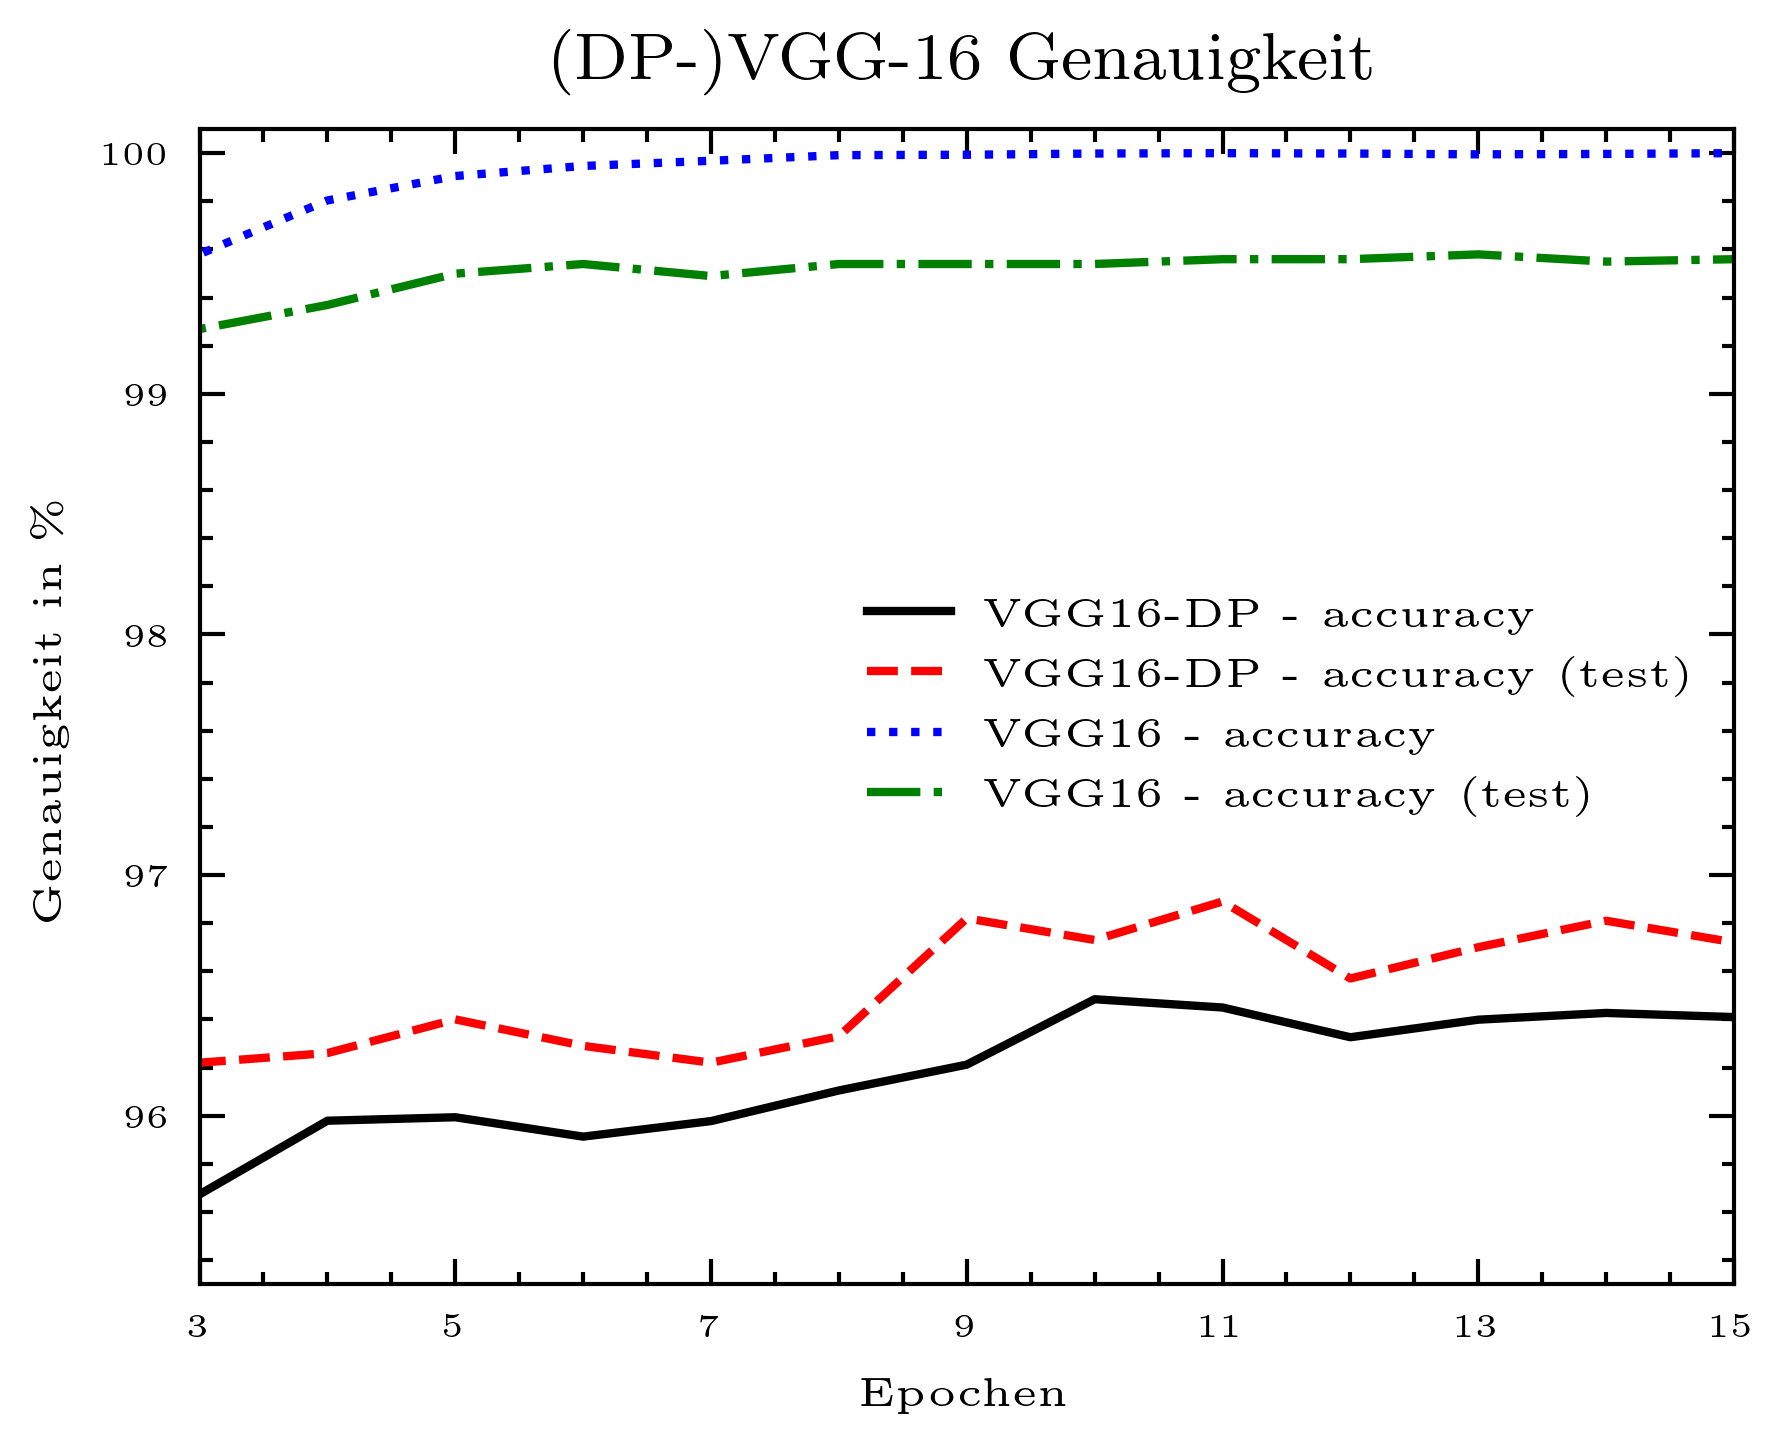
\includegraphics[width=0.5\linewidth]{Bilder/acc.png}
	\caption{Vergleich der Genauigkeit von normal trainiertem und differentiell privatem Modell auf Trainings- und Testdaten des MNIST-Datensatzes}
	\label{img:acc_vgg_dp}
\end{figure}

\begin{figure}[H]
	\centering
	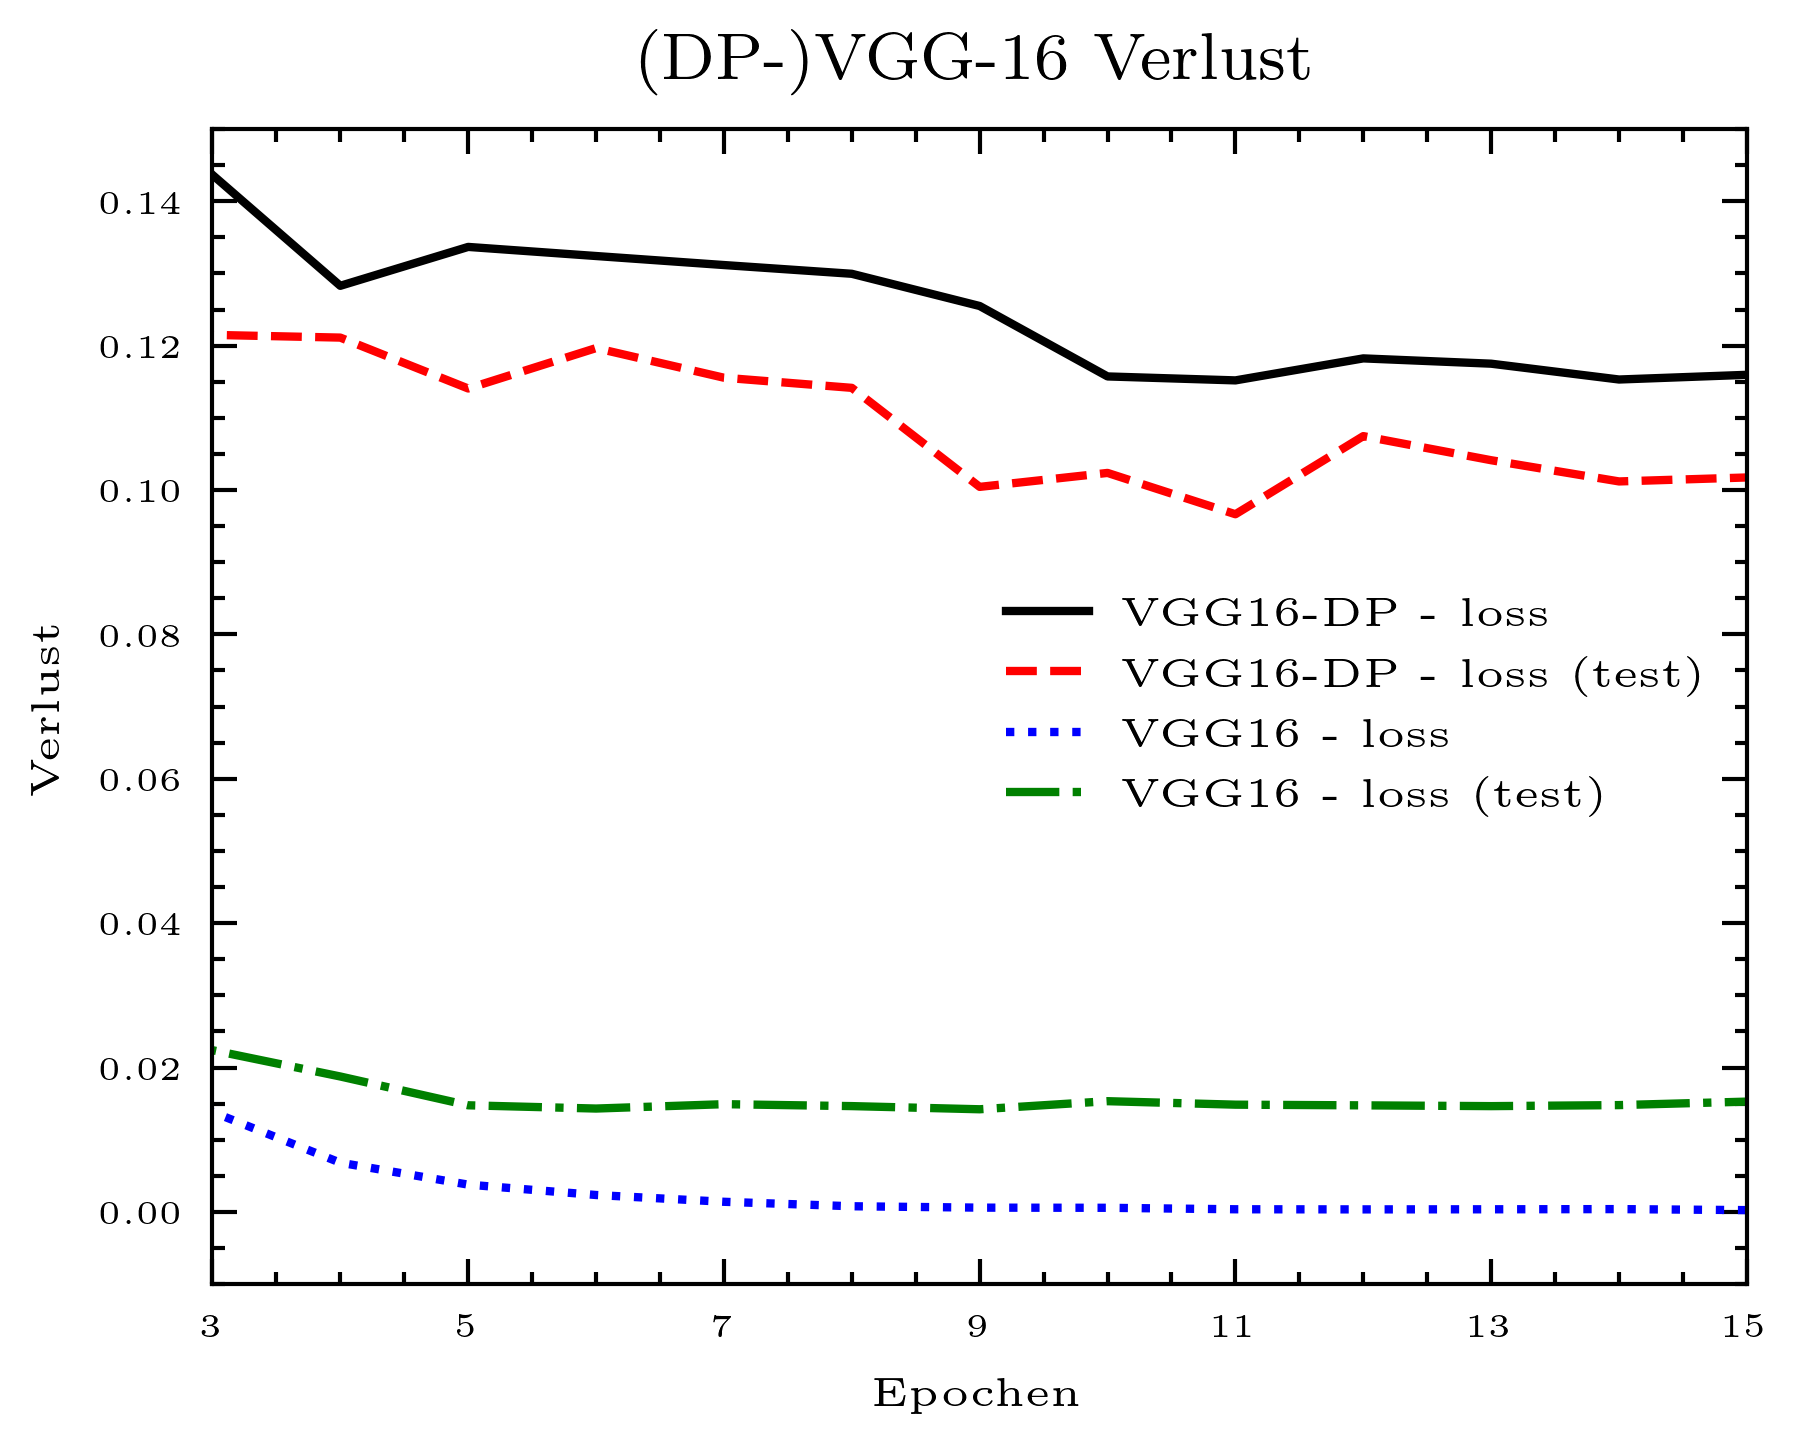
\includegraphics[width=0.5\linewidth]{Bilder/loss.png}
	\caption{Vergleich des Verlusts von normal trainiertem und differentiell privatem Modell auf Trainings- und Testdaten des MNIST-Datensatzes}
	\label{img:loss_vgg_dp}
\end{figure}
Die \textit{Genauigkeit} (\(Acc\)) (Abbildung \ref{img:acc_vgg_dp}) bezüglich der Test- und Trainingsdaten nimmt -- wie erwartet -- im Laufe des Trainingsprozesses zu. 
Diese wird wie folgt definiert: 
\begin{equation}
	Acc = \frac{\text{Anzahl der korrekten Vorhersagen}}{\text{Anzahl der gesamten Vorhersagen}}
\end{equation}
Während das \glqq normale Training\grqq{} mit einer Test-Genauigkeit \(Acc_{\text{test}}\)$\approx99{,}0\%$ startet und bei  \(Acc_{\text{test}}\)$\approx 99{,}5\%$ nach etwa 7 Epochen stagniert, erreicht das \glqq neuronale Netzwerk mit differentieller Privatsphäre\grqq{} zu Beginn einen deutlich niedrigeren Wert von ungefähr $91{,}5\%$ (\(Acc_{\text{test}}\)) und stagniert während der trainierten 15 Epochen bei \(Acc_{\text{test}}\)$\approx96{,}3\%$. Durch den Test eines Trainings auf einer von Google zur Verfügung stehenden GPU-Instanz mit erhöhtem Arbeitsspeicher konnte festgestellt werden, dass die Test-Genauigkeit nach der Durchführung von 15 Epochen auf Basis der aktuellen Parameter nicht weiter erhöht werden kann. Dadurch lässt sich darauf schließen, dass die Methode der differentiellen Privatsphäre in diesem Setup eine Verschlechterung der Klassifikationsqualität des Modells mit sich bringt. Die hohe Genauigkeit des \glqq normalen Modells\grqq{} nach nur einer Trainingsepoche ist auf das Transfer-Learning zurückzuführen, wobei Gewichtungen anhand eines anderen, großen Datensatzes vortrainiert sind, und nicht mit Trainingsstart neu initialisiert werden müssen. Das Qualitätseinbußen der Test-Genauigkeit von Modellen mit differentieller Privatsphäre kann auf das Zugeben von Rauschen zurückgeführt werden.

Der \textit{Verlust} (Abbildung \ref{img:loss_vgg_dp}) während des Trainings zeigt einen ähnlichen Verlauf wie die oben beschriebene Test-Genauigkeit der beiden Modellarten. Nach etwa 7 Epochen beginnt dieser bei der Durchführung des \glqq normalen Trainings\grqq{} zu konvergieren und deutet darauf hin, dass das Training erfolgreich durchgeführt wurde. Auch bei dem \glqq Modell mit differentieller Privatsphäre\grqq{} ist zu beobachten, dass eine Konvergenz der Verlustfunktion nach 15 Epochen zwar eintritt, welche jedoch höher als die des normalen Modells ist.

Das \glqq normale Training\grqq{} kann aufgrund der konvergierenden Verlust- und Genauigkeitswerte nach 7 Epochen beendet werden, da die Parameter nahezu vollständig an den Datensatz angepasst sind. Die Leistung eines mit differentieller Privatsphäre trainierten Klassifikators ist im Gegensatz zu der des \glqq normalen\grqq{} Modells deutlich verschlechtert. Da der Fokus dieser Arbeit nicht auf der Maximierung der Genauigkeit von \glqq verteidigten Modellen\grqq{} lag, wurde dies aufgrund ausreichender Modellqualität nicht weiter geprüft.

\section{Bildqualität}
Aufgrund der verschiedenen Angriffs-Verfahren variiert die Genauigkeit der Bilder in den unterschiedlichen Durchgängen, wobei die Qualität - abhängig von der Komplexität des Generative-Adversarial Networks - gleich ist. Die Genauigkeit des neu generierten Bildes, das aus privaten Daten abgeleitet ist, wird mit Hilfe des Confidence-Scores bezüglich Ziel-Klasse bestimmt. Im Folgenden werden einige Vergleiche über die Bildqualität nach der Ausführung des Angriffs basierend auf einem Klassifizierungsmodell für Zahlen und Gesichtern aufgezeigt.

Die \textit{Qualität} der Bilder ist abhängig von genutztem GAN (Generative adversarial network), das für die Generierung verwendet wird. Generierungen basierend auf dem DCGAN sind aufgrund geringerer Parameter, kürzerer Trainingsdauer und anderer Faktoren qualitativ nicht so hochwertig wie die des genutzten StyleGANs.

\begin{figure}[H]
	\centering
	\begin{subfigure}[b]{0.35\linewidth}
		
\includegraphics[width=\linewidth]{Bilder/0_mnist.png}
		\caption{Generierung der Zahl 0 auf Basis eines DCGAN}
		\label{img:gen_img_dcgan}
	\end{subfigure}
	\hspace{1cm} % Einfügen von horizontalen Abständen zwischen den Bildern
	\begin{subfigure}[b]{0.35\linewidth}
		
\includegraphics[width=\linewidth]{Bilder/401_celeba.png}
		\caption{Generierung einer Frau mit Hilfe eines StyleGANs}
		\label{img:gen_img_stylegan}
	\end{subfigure}
	\caption{Bildqualität der GAN-Modelle}
	\label{img:gen_img}
\end{figure}
Die Bilder des DCGAN basierten Generators sind etwas schwach mit vergleichsweise wenigen Pixeln aufgelöst (siehe Abbildung \ref{img:gen_img_dcgan}). Dahingegen lassen sich Bilder des StyleGAN Netzwerks in einer deutlich besseren Auflösung von bis zu 200 $\times$ 200 Pixeln generiern. Wie in Abbildung \ref{img:gen_img_stylegan} zu erkennen, wird die Qualität der Bilder durch die Reduktion der Pixel deutlich verschlechtert, was aber zu einer effektiveren Angriffsdauer führt. Im Gegensatz zu den generierten Ziffern handelt es sich bei den Gesichtern um 3-Kanal Bilder (RGB), weshalb diese farblich zu betrachtet sind.
\section{Bewertung der Angriffsleistung}
Dieses Kapitel befasst sich mit der Auswertung beider Angriffe nach der Durchführung, wobei im Folgenden ein Vergleich mit dem Ziel der Stärken- und Schwächenbeleuchtung aufgestellt wird. Um die Angriffe besser bewerten zu können, werden zum einen visuelle, aber auch metrische Qualitätsmerkmale begutachtet, wozu beispielsweise die Genauigkeit der neu generierten Bilder bezüglich der Ziel-Kategorie des \glqq angegriffenen\grqq{} Modells zählt.
\subsection{Genauigkeit der Angriffe}
Um eine präzisere Analyse der Angriffsgenauigkeit zu ermöglichen, werden neben visuellen Metriken auch numerische Kennzahlen integriert, um einen messbaren und vergleichbaren Wert zu erlangen.

Im Zuge der Durchführung eines \glqq KEDMI\grqq-Angriffs auf ein Zielmodell, das für die Klassifikation von handgeschriebenen Ziffern konzipiert ist, wurden entscheidende Erkenntnisse gewonnen, welche die potenzielle Gefahr des Angiffs verdeutlichen und die Notwendigkeit, adäquate Verteidigungsstragegien zu implementieren, unterstreichen. Im Folgenden werden verschiedene Metriken präsentiert, die im Rahmen der Evaluierung Verwendung finden und einen direkten Vergleich zu \glqq RBMI\grqq-Angriffen ermöglichen. Diese bieten Einblicke in die Wirksamkeit, Effektivität und Effizienz der Angriffe sowie die daraus resultierenden Auswirkungn auf die Sicherheits-Komponente des Zielmodells. Die detaillierte Analyse der Evaluierungsmetriken ermöglicht eine Bewertung der durch den Angriff aufkommenden Schwachstelle. Diese Ergebnisse dienen zudem als Grundlage für die Ableitung geeigneter Schutzmaßnahmen zur Stärkung der Sicherheit und Robustheit des Modells gegenüber Inferenz-Angriffen.

Die visuelle Metrik zur Bewertung der Angriffsqualität stellt einen Vergleich der wiederhergestellten Bilder nach erfolgreicher Durchführung auf ein bestimmtes Zielmodell dar. Dafür werden 60 Bilder aus insgesamt 10 Klassen, die während des Angriffs generiert wurden, mit einer Sammlung von 60 Originalbildern der selben Klasse gegenübergestellt, um diese zu vergleichen. Das Angriffsziel besteht darin, dass Merkmale der Originalbilder visuell mit denen der generierten Bilder übereinstimmen, jedoch nicht jeder einzelne Trainings-Datenpunkt generiert wird.

\begin{figure}[H]
	\centering
	\begin{subfigure}[b]{0.35\linewidth}
		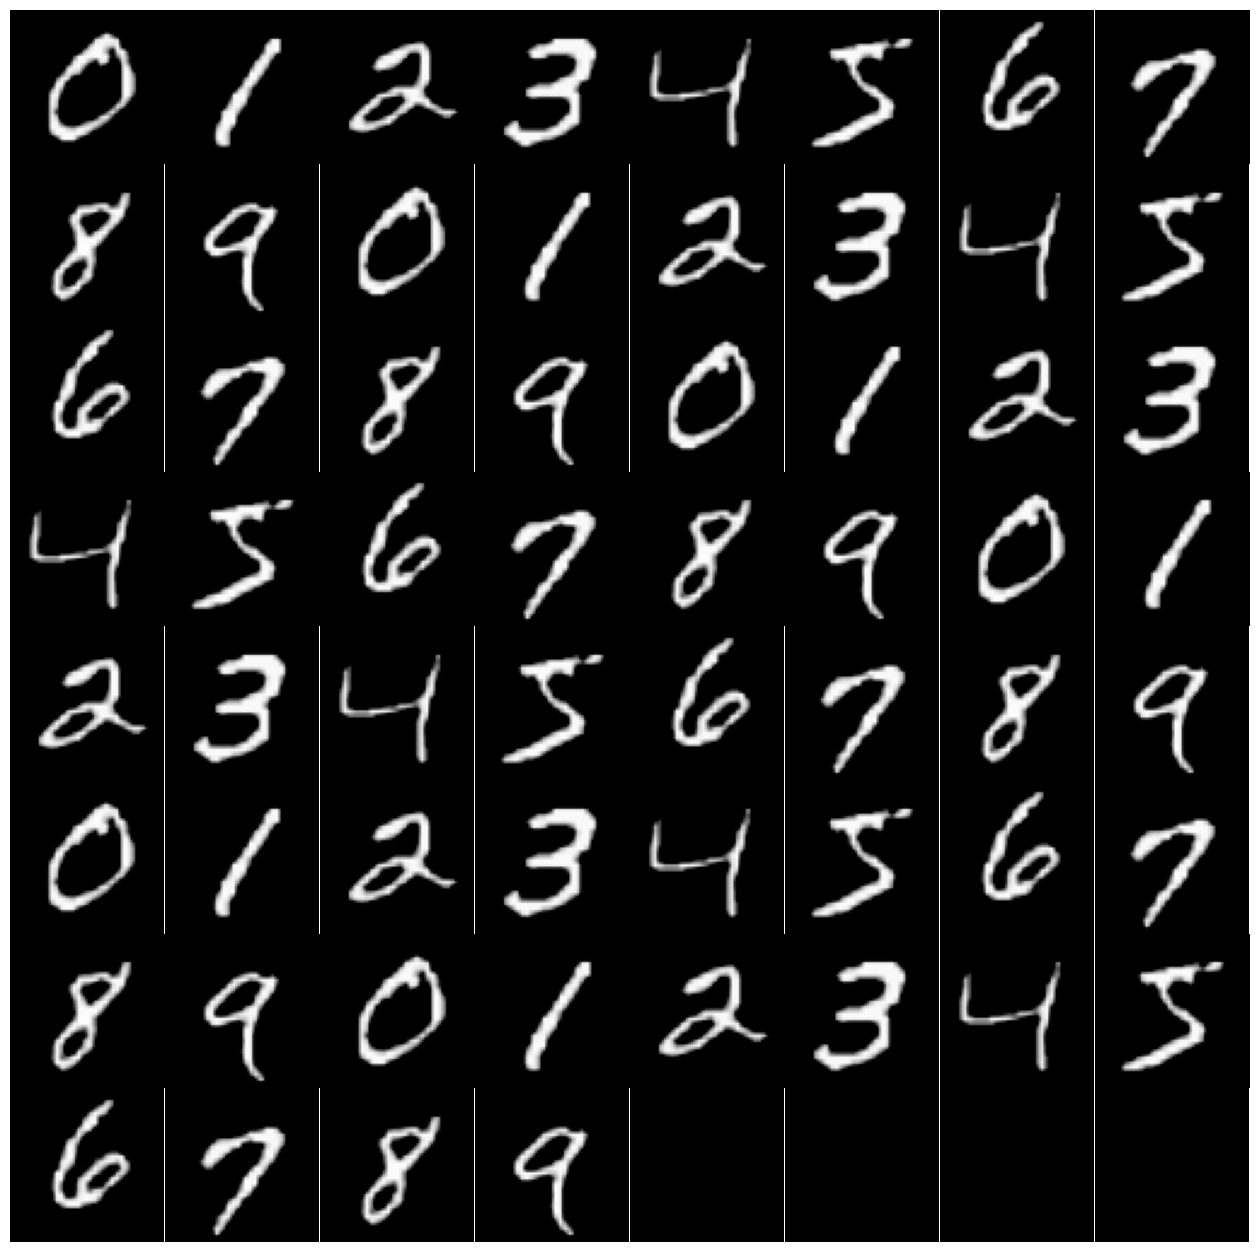
\includegraphics[width=\linewidth]{Bilder/mnist_orig.png}
		\caption{60 Originalbilder des MNIST-Datensatzes}
		\label{img:kedmi_orig}
	\end{subfigure}
	\hspace{1cm} % Einfügen von horizontalen Abständen zwischen den Bildern
	\begin{subfigure}[b]{0.348\linewidth}
		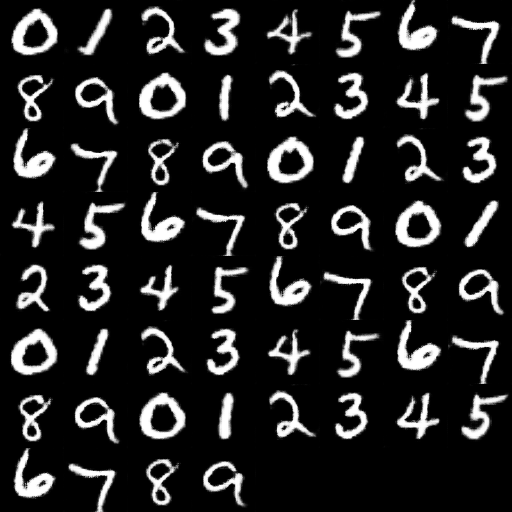
\includegraphics[width=\linewidth]{Bilder/kedmi_mnist.png}
		\caption{60 durch den \glqq KEDMI\grqq-Angriff generierte Bilder}
		\label{img:kedmi_gen}
	\end{subfigure}
	\caption{Gegenüberstellung originaler und generierter Ziffern}
	\label{img:kedmi_visual}
\end{figure}

Es zeigt sich deutlich, dass alle Klassen durch eine konsistente Übereinstimmung zwischen den originalen Bildern (siehe Abbildung \ref{img:kedmi_orig}) des Datensatzes und den generierten Bildern des \textit{"KEDMI"}-Angriffs (siehe Abbildung \ref{img:kedmi_gen}) korrekt wiederhergestellt wurden. Beim Bildvergleich wird ersichtlich, dass die Aufmachung der originalen zu den generierten Bildern variiert, was auf den Trainingsprozess und die Qualität des genutzten Generator-Netzwerks (GAN) zurückzuführen ist. Beispielsweise sind die generierten Ziffern deutlich kräftiger, als die Originalzahlen. Zudem ist erkennbar, dass die Bilder nicht exakt identisch sind, was jedoch nicht das Ziel des Angriffs darstellt, da die Bilder eine durchschnittliche Repräsentation der Features eines bestimmten Labels symbolisieren sollen.

\begin{figure}[H]
	\centering
	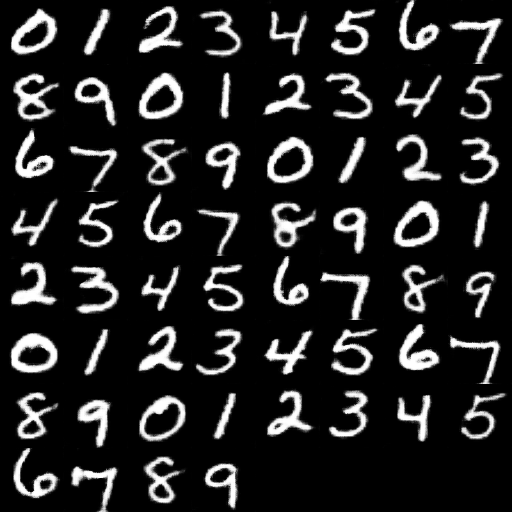
\includegraphics[width=0.35\linewidth]{Bilder/qmnist.png}
	\caption{Angriffsgenerierungen auf Basis eines QMNIST-Generators}
	\label{img:kedmi_qmnist}
\end{figure}

Eine zusätzliche Darstellung der Ergebnisse bezüglich Ziffern (siehe Abbildung \ref{img:kedmi_qmnist}) zur visuellen Qualitätsbewertung wurde auf Grundlage eines Generators erstellt, der mittels QMNIST-Daten trainiert wurde. Die zugrundeliegenden Originalbilder sind in Abbildung \ref{img:kedmi_orig} zu finden. Diese Resultate illustrieren die Präzision des durchgeführten Angriffs, bei dem private Daten, welche für das Training verwendet wurden, unbekannt sind. In diesem Kontext zeigt sich erneut eine nahezu hundertprozentige Genauigkeit der Ergebnisse im Bezug auf das Zielmodell. Diese Feststellung unterstreicht die Effektivität des angewandten Angriffsmechanismus, selbst in Fällen, in denen spezifische Trainingsdaten nicht explizit bekannt sind.

Die visuelle Qualitätsanalyse bezüglich eines weiteren Datensatzes (CelebA) gestaltet sich aufgrund der komplexeren Datenpunktstruktur etwas unklarer im Vergleich zu den auf MNIST basierenen Angriffsgenerierungen. Die Bildqualität des verwendeten Generators (GAN) ist die komplexität der Merkmale signifikant beeinträchtigt. Auch hier werden 60 verschiedene Bilder (je eins pro Kategorie) mit dem jeweiligen Originalen der gleichen Klasse verglichen.

\begin{figure}[H]
	\centering
	\begin{subfigure}[b]{0.35\linewidth}
		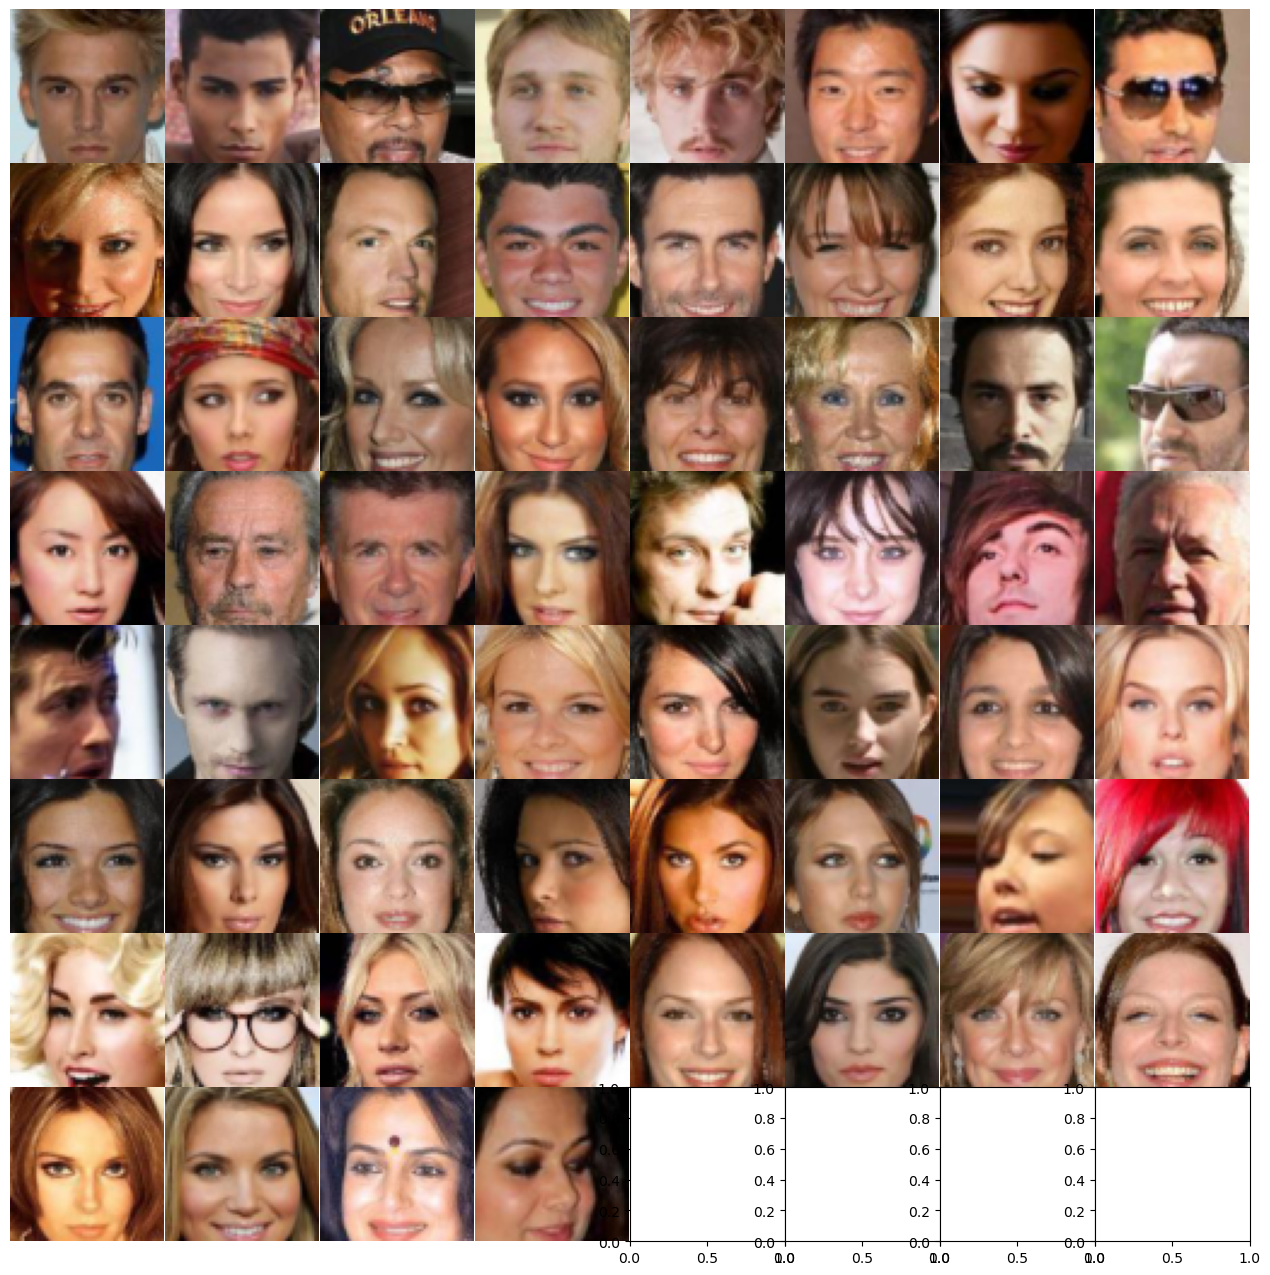
\includegraphics[width=\linewidth]{Bilder/celeba_orig.png}
		\caption{60 Originalbilder des CelebA-Datensatzes}
		\label{img:kedmi_celeba_orig}
	\end{subfigure}
	\hspace{1cm} % Einfügen von horizontalen Abständen zwischen den Bildern
	\begin{subfigure}[b]{0.348\linewidth}
		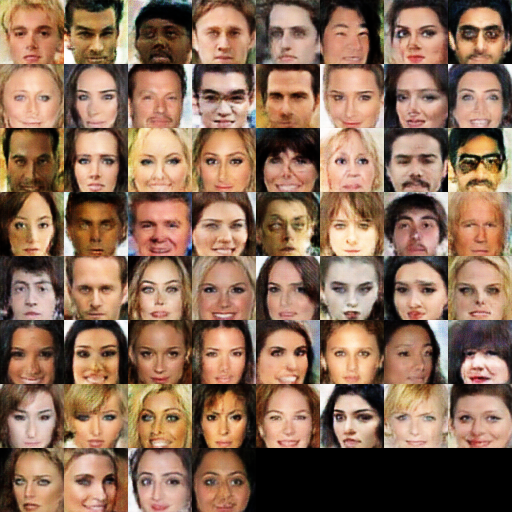
\includegraphics[width=\linewidth]{Bilder/kedmi_celeba.png}
		\caption{60 durch den \glqq KEDMI\grqq-Angriff generierte Bilder}
		\label{img:kedmi_celeba_gen}
	\end{subfigure}
	\caption{Gegenüberstellung originaler und generierter Gesichter}
	\label{img:kedmi_celeba_visuell}
\end{figure}

Bei der Durchführung des \glqq KEDMI\grqq-Angriffs auf einen für Gesichtsdaten trainierten Klassifizierer ist klar erkennbar, dass die zugrundeliegende Person, wenn auch teilweise verzerrt, wiederhergestellt wurde. Die Verzerrung und die daraus resultierende Ungenauigkeit in bestimmten Details sind auf die Bildqualität des generierenden Netzwerks zurückzuführen, das auch bei einfacher Generierung unabhängig von Angriffen Bildfehler einschleust. Es wird ebenfalls deutlich, dass die verschiedenen Bilder nicht vollständig mit dem Original übereinstimmen, da beispielsweise Personen in die \glqq falsche\grqq{} Richtung schauen. Dies ist darauf zurückzuführen, dass der Angriff nicht auf die eindeutige Generierung aller im Training verwendeten Datenpunkte abzielt, sondern auf ein Bild mit maximiertem Confidence-Score bezüglich der Zielklasse, damit dieses vom Klassifizierer mit hoher Sicherheit richtig erkannt wird, um darauf basierend die wichtigsten Features der jeweiligen Klasse symbolisieren zu können. 

Im Gegensatz zu \glqq KEDMI\grqq-Angriffen stellen \glqq RBMI\grqq-Angriffe eine größere Herausforderung bedingt durch die komplexere Angriffsdurchführung dar. 

Mit Hilfe der visuellen Metrik kann auch hier ein Vergleich zwischen generierten und originalen Daten hergestellt werden, um einen Teil der \textit{Angriffsqualität} darstellen zu können. Hierzu werden zehn Originalbilder mit einem durch den Angriff generierten Zielbild verglichen, um eine visuelle Qualitätsschätzung durchführen zu können. Auch hier ist das Ziel des Angriffs, einen \glqq Durchschnittsdatenpunkt\grqq{} zu generieren, der die Features des jeweiligen Ziellabels am besten repräsentiert und somit eine hohe Genauigkeit bezüglich der Zielklasse des Modells hat. 

\begin{figure}[H]
	\centering
	\begin{subfigure}[b]{0.8\linewidth}
		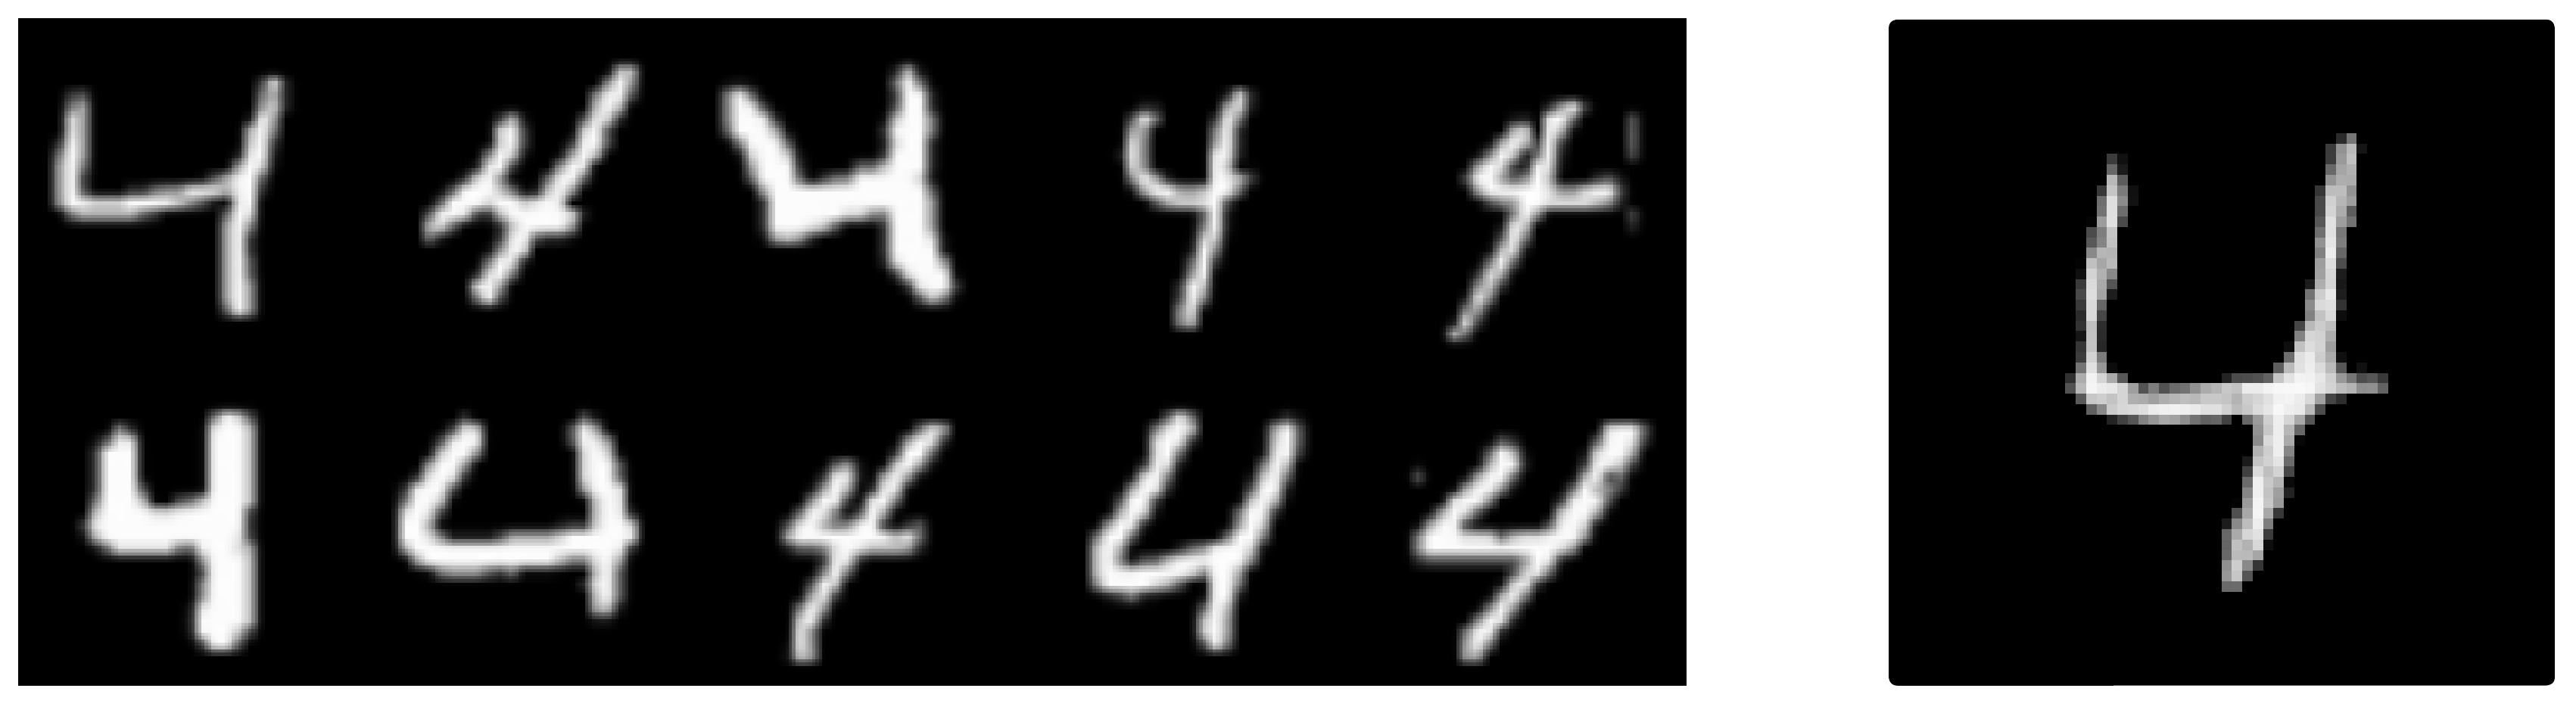
\includegraphics[width=\linewidth, height=5cm, keepaspectratio]{Bilder/4_mnist_rbmi.png}
	\end{subfigure}
	\caption{Gegenüberstellung von Originalbildern des MNIST-Datensatzes (\textit{links}) mit dem generierten Bild (\textit{rechts}) (durch \glqq RBMI\grqq-Angriff) der Zielklasse \glqq 4\grqq{}}
	\label{img:rbmi_visual_mnist}
\end{figure}

Während der Durchführung von Algorithmen zur Rückgewinnung von Trainingsdaten fällt auf, dass der BlackBox-basierte \glqq RBMI\grqq-Angriff Bilder generiert, die in jeder Klasse visuell korrekte Darstellungen hervorbringen. Diese Beobachtung basiert auf einem Vergleich zwischen den generierten und den originalen Bildern (aus Abbildung \ref{img:rbmi_visual_mnist}). Deutlich erkennbar ist, dass die zurückgewonnenen Bilder mit den Originalbildern in Übereinstimmung stehen. Diese Übereinstimmung manifestiert sich in einer hohen \textit{visuellen Angriffsqualität}, die mit jener des \glqq KEDMI\grqq-Angriffs vergleichbar ist.

\begin{figure}[H]
	\centering
	\begin{subfigure}[b]{0.8\linewidth}
		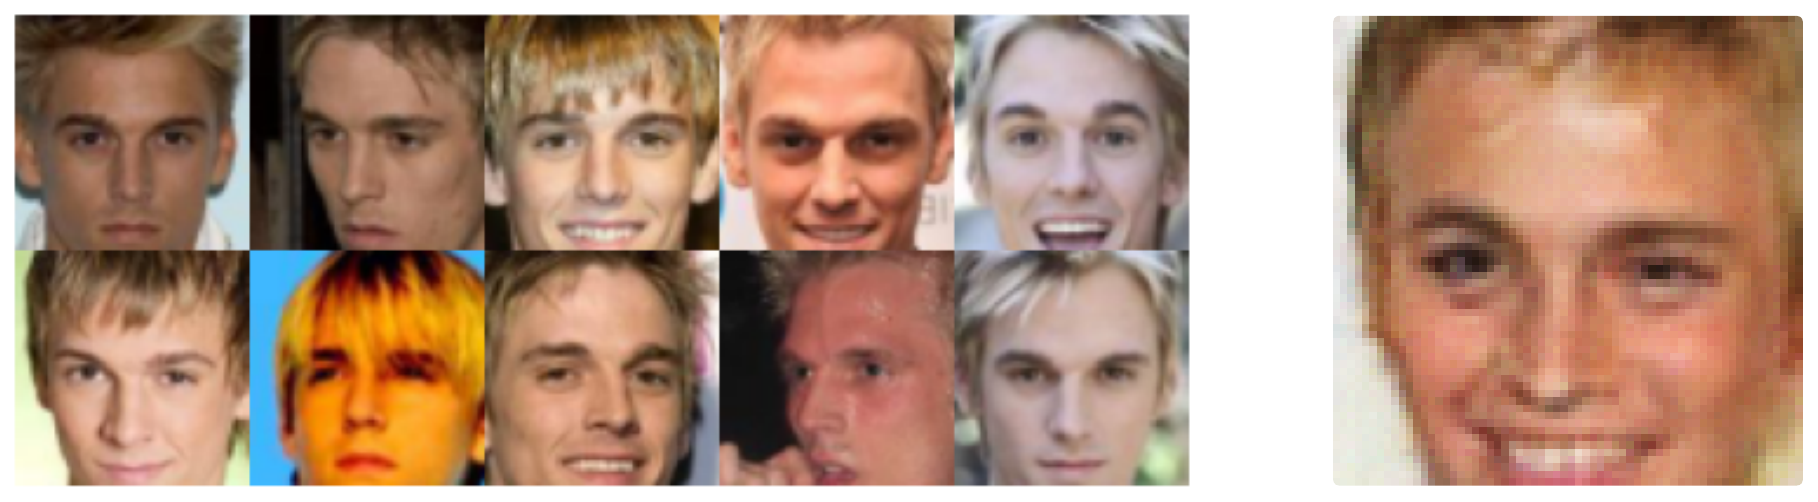
\includegraphics[width=\linewidth, height=5cm, keepaspectratio]{Bilder/0_celeba_rbmi.png}
	\end{subfigure}
	\caption{Gegenüberstellung von Originalbildern des CelebA-Datensatzes (\textit{links}) mit dem generierten Bild (\textit{rechts}) (durch \glqq RBMI\grqq-Angriff) der Zielperson}
	\label{img:rbmi_visual}
\end{figure}

Für die Angriffsvalidierung werden auch hier (Abbildung \ref{img:rbmi_visual}) Originalbilder mit Generierungen basierend auf den CelebA-Datensatz verglichen. Das rechte Bild wurde durch die Ausführung eines \glqq RBMI\grqq-Angriffs unter Verwendung des DCGAN-Generators generiert. Die Qualität der erzeugten Bilder ist unmittelbar mit der Generierungsfähigkeit des Generators verbunden. Da der Generator lediglich Bilder mit einer Größe von 64 $\times$ 64 Pixeln erstellen kann, bleibt die Auflösung der rückgenerierten Bilder entsprechend begrenzt. Deutlich zu erkennen ist allerdings, dass das generierte Bild mehrere Features aus den verschiedenen Trainingsbildern darstellt und dadurch auf eine positive Angriffsdurchführung hindeutet.

\begin{figure}[H]
	\centering
	\begin{subfigure}[b]{0.8\linewidth}
		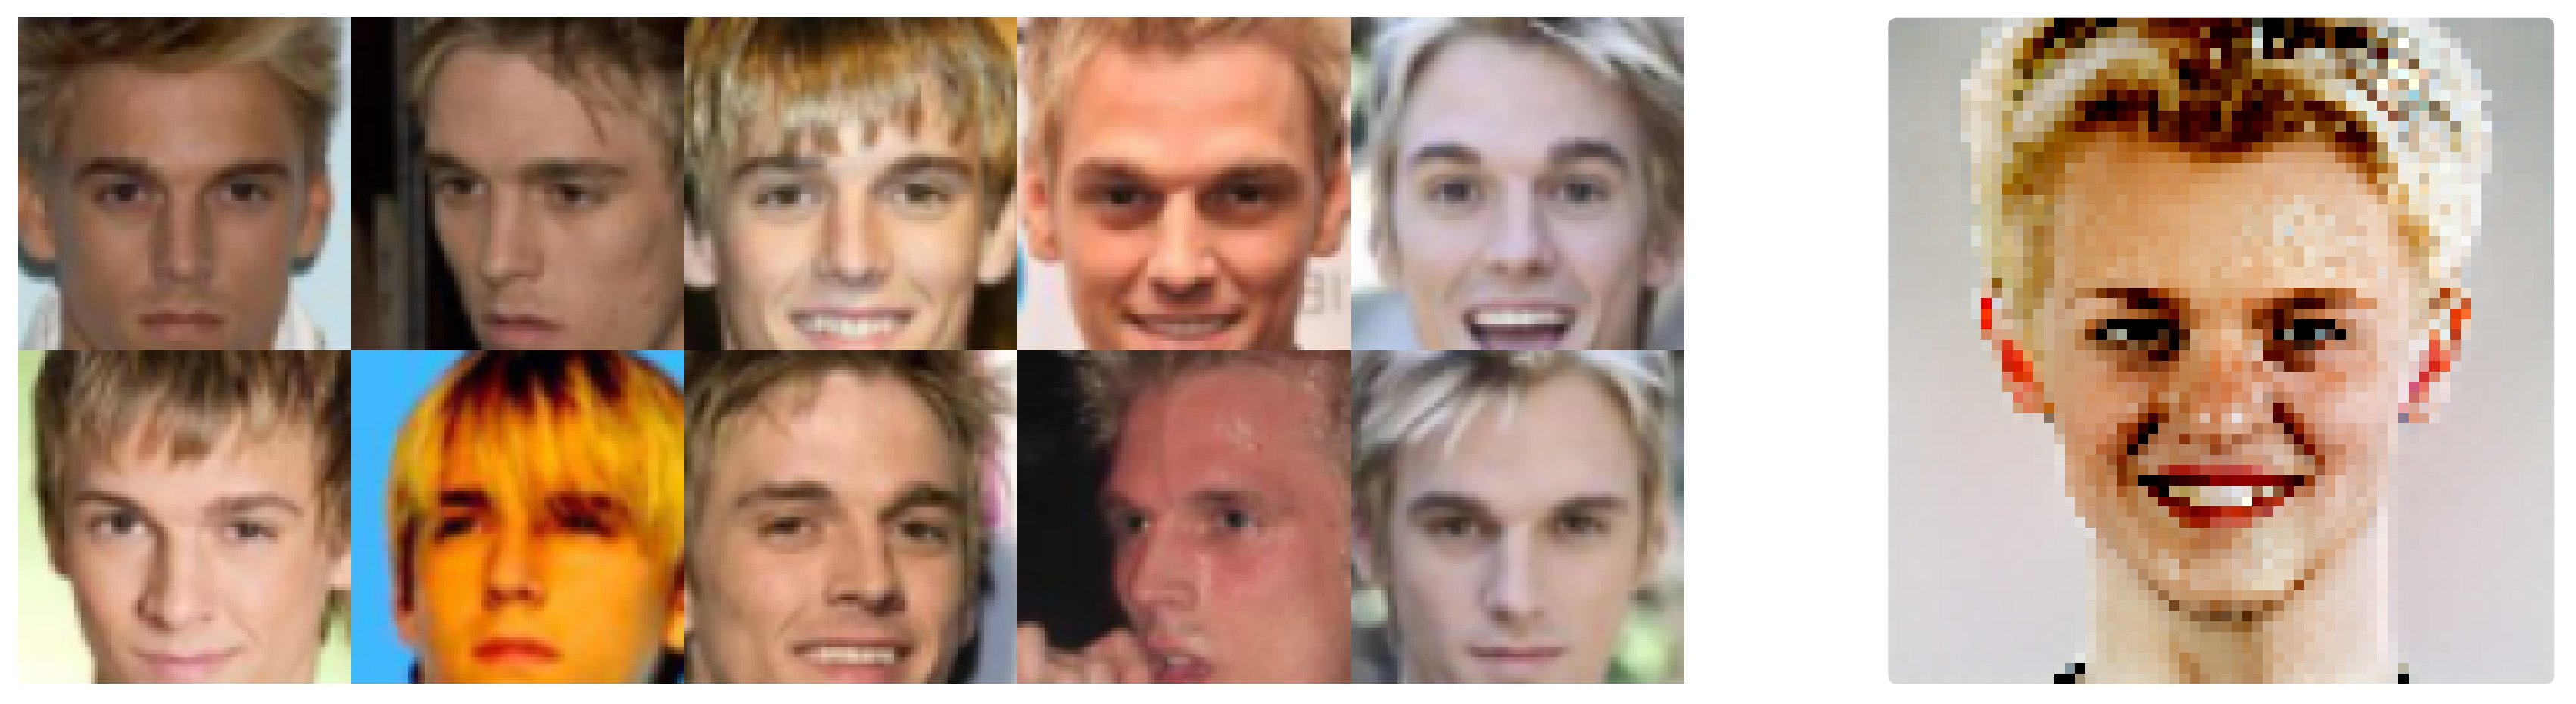
\includegraphics[width=\linewidth, height=5cm, keepaspectratio]{Bilder/0_celeba_rbmi_stylegan.png}
	\end{subfigure}
	\caption{Gegenüberstellung von Originalbildern des CelebA-Datensatzes (\textit{links}) mit dem generierten Bild (\textit{rechts}) (durch \glqq RBMI\grqq-Angriff und StyleGAN) der Zielperson}
	\label{img:rbmi_visual_stylegan}
\end{figure}

Um die \textit{Qualität} des Angriffs auf visueller und statistischer Ebene eingehender zu analysieren, wurde ein Generator basierend auf der Style-GAN-Architektur verwendet, der auf einem unabhängigen Datensatz trainiert ist (\cite{noauthor_nvlabsffhq-dataset_2023}). Dieser Ansatz ermöglicht eine umfassendere Bewertung der erzeugten Bilder, wobei visuelle und statistische Merkmale gleichermaßen berücksichtigt werden.

Die Abbildung \ref{img:rbmi_visual_stylegan} illustriert, dass der Generationsprozess mittels des Style-GAN-Generators zu Bildern führt, die die repräsentativen Merkmale der Originalperson aufweisen. Beispiele hierfür sind unter anderem die blonden Haare und andere charakteristische Eigenschaften wie Ohren. Es ist anzumerken, dass das neu generierte Gesicht eine höhere Auflösung aufweist, die aufgrund der besseren Qualität des Generators erzielt wird. Während des Algorithmus wird diese Auflösung jedoch auf 64 $\times$ 64 Pixel reduziert, um eine effiziente Ausführung zu gewährleisten.

Die hohe Auflösung des generierten Gesichts, kombiniert mit der Integration von Merkmalen aus mehreren Trainingsbildern, verdeutlicht die anspruchsvolle Generierung von Bildern durch den \glqq RBMI\grqq-Angriff unter Verwendung des Style-GAN-Generators. Dieser Ansatz zeugt von einer verbesserten visuellen Qualität und statistischen Relevanz im Vergleich zu einfachen Generatoren, was die Notwendigkeit betont, solche fortgeschrittenen Techniken bei der Entwicklung von Verteidigungsstrategien gegen Modellinversionsangriffe zu berücksichtigen. Zudem bietet er die Möglichkeit der Generierung von Trainingsdaten, ohne dabei den genauen Datensatz zu kennen.

Die visuelle Angriffsqualität wird dabei als Kriterium herangezogen, um die visuelle Ähnlichkeit zwischen den generierten und den originalen Bildern zu bewerten. Diese Qualität ist bei dem \glqq RBMI\grqq-Angriff als hoch einzustufen, was darauf hinweist, dass die rückgewonnenen Bilder die visuellen Merkmale und Strukturen der Originalbilder präzise wiedergeben. Dieses Phänomen findet Analogie zu der Beobachtung, die bereits beim \glqq KEDMI\grqq-Angriff festgestellt wurde.

Die visuelle Übereinstimmung zwischen generierten und originalen Bildern ist ein entscheidendes Kriterium für die Wirksamkeit von Modellinversionsangriffen, insbesondere im Hinblick auf die Erhaltung von Klassenmerkmalen und Strukturdetails. Die hohe visuelle Angriffsqualität beider Algorithmen deutet darauf hin, dass diese Ansätze eine erfolgreiche Rückgewinnung von Trainingsdaten ermöglichen und somit potenzielle Risiken für die Sicherheit und Vertraulichkeit von Modellen darstellen.
\subsection{Angriffsstatistiken}
%KEDMI
Um über visuelle Qualitätsmerkmale hinaus zusätzliche Metiken einführen zu können, werden im Folgenden detaillierte Vergleiche durch verschiedene Statistiken mit dem Ziel des Angriffvergleichs und der Auflistung von Leistungsfähigkeiten präsentiert. Besondere Aufmerksamkeit wird dabei auf die Angriffsdauer und die Genauigkeit der Angriffe gelegt. Durch die Anwendung statistischer Methoden wird ein systematischer Vergleich der Angriffsleistungen ermöglicht, wobei eine Analyse dieser statistischen Parameter eine Rückschlussziehung bezüglich der Leistungsfähigkeit der Angriffe bietet.

Des Weiteren wird die Genauigkeit der Angriffe als entscheidende Metrik betrachtet. Dadurch soll die visuelle Einstimmigkeit zwischen Generierung und Originalbild belegt werden, indem man Kennzahlen über die Genauigkeit der Vorhersage des Zielmodells interpretiert. Diese Erkenntnisse tragen dazu bei, die Wirksamkeit der Angriffe in verschiedenen Kontexten zu bewerten und möglicherweise Optimierungspotenziale zu identifizieren.

\begin{table}[h]
	\centering
	\renewcommand{\arraystretch}{1.5}
	\resizebox{\textwidth}{!}{
		\begin{tabular}{|c|c|c|c|c|c|c|}
			\hline
			\textbf{Modell-Art} & \textbf{Generator} & \textbf{Datensatz} & \textbf{Iterationen} & \textbf{Dauer pro Iteration} & \textbf{Gesamtdauer} & \textbf{Genauigkeit}\\
			\hline
			\textit{VGG-16} & DCGAN & MNIST & 2.400 & 0,11 sec & 4 min & \textbf{100,0\%}\\
			\hline
			\textit{VGG-16} & DCGAN & CelebA & 2.400 & 0,12 sec & 4 min & \textbf{100,0\%}\\
			\hline
		\end{tabular}
	}
	\caption{\glqq KEDMI\grqq-Angriffsstatistik}
	\label{tab:kedmi_stats}
\end{table}

Die Tabelle \ref{tab:kedmi_stats} präsentiert einen detaillierten Vergleich hinsichtlich der Ausführung des \glqq KEDMI\grqq-Angriffs zwischen dem MNIST- und dem CelebA-Datensatz. Die Resultate verdeutlichen, dass die zeitliche Komponente der Angriffe lediglich um wenige Millisekunden pro Iteration varriert, was auf die Anwendung desselben Algorithmus, identischer Bildgröße und einer gleichbleibenden GAN-Architektur zurückzuführen ist. In diesem Zusammenhang wurden vordefinierte 2.400 Iterationen pro Rückgenerierung verwendet, um eine maximal mögliche Genauigkeit zu gewährleisten. Diese erreicht bei beiden Angriffen einen Wert von 100\%, was auf eine korrekte Klassifikation der generierten Bilder durch das Zielmodell hindeutet. 

Die 100\%ige Genauigkeit erstreckt sich über die Rückgewinnung von vergleichsweise simplen Datenpunkten aus dem MNIST-Datensatz bis hin zu Datenpunkten mit komplexeren Merkmalen, wie beispielsweise Gesichtsbildern des CelebA-Datensatzes. Dies bezeugt die Robustheit und Wirksamkeit des \glqq KEDMI\grqq-Angriffs über verschiedene Datensätze und verdeutlicht die Fähigkeit des Algorithmus, eine akkurate Bildqualität und Übereinstimmung zwischen Generierung und Original, unabhängig von der Datenkomplexität, sicherzustellen, wobei Modell und Daten bekannt sind.

Die Konsistenz der Genauigkeit in verschiedenen Kontexten unterstreicht die Zuverlässigkeit des \glqq KEDMI\grqq-Angriffs und legt nahe, dass dieser Ansatz auch in komplexeren Szenarien anwendbar ist. Diese Erkenntnisse ermöglichen nicht nur eine tiefgehende Bewertung der Angriffsleistung, sondern bieten auch Einblicke in die Generalisierbarkeit über unterschiedliche Datensätze und Merkmalskomplexitäten hinweg.
%RBMI
\begin{table}[h]
	\centering
	\renewcommand{\arraystretch}{1.5}
	\resizebox{\textwidth}{!}{
		\begin{tabular}{|c|c|c|c|c|c|c|}
			\hline
			\textbf{Modell-Art} & \textbf{Generator} & \textbf{Datensatz} & \textbf{Iterationen} & \textbf{Dauer pro Iteration} & \textbf{Gesamtdauer} & \textbf{Genauigkeit}\\
			\hline
			\textit{VGG-16} & DCGAN & MNIST & 40.000 & 0,018 sec & 12 min & \textbf{100,0\%}\\
			\hline
			\textit{VGG-16} & DCGAN & CelebA & 40.000 & 0,024 sec & 16 min & \textbf{99,94\%}\\
			\hline
			\textit{VGG-16} & StyleGAN & FFHQ & 100.000 & 0,085 sec & 142 min & \textbf{98,44\%}\\
			\hline
		\end{tabular}
	}
	\caption{\glqq RBMI\grqq-Angriffsstatistik}
	\label{tab:rbmi_stats}
\end{table}

Die Tabelle \ref{tab:rbmi_stats} verdeutlicht die Angriffsstatistik des \glqq RBMI\grqq-Angriffs. Auch dieser Angriff wurde in verschiedenen Szenarien auf seine Wirksamkeit hin getestet, und die Ergebnisse werden in Form von Metriken dokumentiert. Die Untersuchung zeigt, dass der \glqq RBMI\grqq-Angriff in verschiedenen Kontexten konsistente und überzeugende Ergebnisse liefert. Die Metriken spiegeln die Effektivität des Angriffs wider und bieten Einblicke in seine Leistungsfähigkeit auf Basis unterschiedlicher Bedingungen. Während des Angriffs wurden verschiedene Testläufe durchgeführt, wobei sowohl einfache als auch komplexe Datenpunkte berücksichtigt wurden. Zusätzlich zu den in der \glqq KEDMI\grqq-Statistik (Tabelle \ref{tab:kedmi_stats}) befindlichen Angriffen wurde hier auch ein weiteres Szenario getestet. Dieses umfasst einen Angriff ohne das Kennen des eigentlichen Datensatzes. Dabei wurde ein Generator verwendet, der auf Basis des FFHQ-Datensatzes (\cite{noauthor_nvlabsffhq-dataset_2023})  trainiert ist. 

Die erzielten Ergebnisse weisen darauf hin, dass der \glqq RBMI\grqq-Angriff in der Lage ist, genaue Klassifikationen, unabhängig von Komplexität der betrachteten Daten, zu erreichen. Dies belegt die Robustheit und Anpassungsfähigkeit des Angriffsalgorithmus an verschiedene Datensätze. Insbesondere wurden Metriken verwendet, um den Fortschritt und die Genauigkeit des Angriffs zu quantifizieren. Die erzielten Ergebnisse verdeutlichen, dass der \glqq RBMI\grqq-Angriff nicht nur in der Lage ist, sich an unterschiedliche Datensätze anzupassen, sondern auch eine konstante und zuverlässige Leistung in verschiedenen Szenarien aufweist. Hervorzuheben ist hierbei, dass auf Basis eines komplexen Generators (StyleGAN), der mit vom Zielmodell unabhängen Daten trainiert ist, ein sehr hohe Genauigkeit in Betracht auf die Zielklasse erreicht wurde, ohne dabei Parameter des Modells zu kennen.

Um einen Vergleich zwischen den beiden Angriffsmethoden, KEDMI und RBMI, anzustellen, werden sowohl die Dauer des Angriffs als auch die Genauigkeit betrachtet. Die Analyse der Angriffsqualität legt nahe, dass beide Methoden in der Lage sind, hochwertige Generierungen basierend auf den zugrunde liegenden Trainingsdaten zu erstellen, wobei unterschiedliche Algorithmen zum Einsatz kommen. Der KEDMI-Angriff weist lediglich den Nachteil auf, dass er auf Whitebox-Prinzipien basiert und somit Zugang zu Modellparametern und Trainingsdaten erfordert. Im Gegensatz dazu ist der RBMI-Angriff blackbox-basiert und kann auf jedes Modell angewendet werden, dessen Outputklassen bekannt sind und ein ähnlicher Datensatz vorhanden ist. Ein Nachteil des RBMI-Angriffs besteht jedoch in der Dauer, da dieser einerseits mehr Zeit pro Iteration beansprucht und andererseits eine deutlich höhere Anzahl von Iterationen erfordert.

In qualitativer Hinsicht zeigen beide Angriffe Ähnlichkeiten. Die Güte des Ergebnisses korreliert positiv mit der Bildqualität des Generators. Allerdings verlängert sich die Dauer des RBMI-Angriffs mit zunehmender Bildqualität, wie aus der letzten Zeile der Tabelle \ref{tab:rbmi_stats} hervorgeht. In diesem speziellen Fall wurde eine Genauigkeit von über 98\% erst nach 100.000 Iterationen erreicht, was der Durchführung des Angriffalgorithmus geschuldet ist. Es ist anzumerken, dass die höhere Iterationsanzahl zu einer verbesserten Genauigkeit führt, jedoch auch die Gesamtdauer des Angriffs erheblich verlängert.
% Genauigkeit normal
% Dauer
\section{Auswertung der Verteidigungsstrategie}\label{chpt:dpnn_stats}
% Genauigkeit dp
Das folgende Unterkapitel widmet sich der umfassenden Auswertung der Verteidigungsstrategie "Differential Privacy". Ziel ist es, die Sinnhaftigkeit dieser Strategie zu bewerten und insbesondere zu untersuchen, wie sich die Integration von Differential Privacy während des Trainingsprozess auf die Genauigkeit von Angriffen auswirkt. Differential Privacy ist eine vielversprechende Methode zum Schutz von Datenschutz und Sicherheit in maschinellen Lernmodellen. Hier werden verschiedene Aspekte analysiert, darunter die Effektivität der Differential Privacy in der Verteidigung gegenüber Angriffen sowie mögliche Auswirkungen auf die Genauigkeit von Angriffen und Klassifikationen. Die Untersuchung berücksichtigt sowohl quantitative Metriken als auch qualitative Aspekte, um ein umfassendes Bild der Wirksamkeit dieser Verteidigungsstrategie zu erhalten. Ziel ist es, zu bewerten, inwieweit Differential Privacy als sinnvoller Schutzmechanismus für maschinelle Lernmodelle fungiert und welche Auswirkungen dies auf die Präzision von Angriffen und Klassifikationen hat.

\begin{figure}[H]
	\centering
	\begin{subfigure}[b]{0.35\linewidth}
		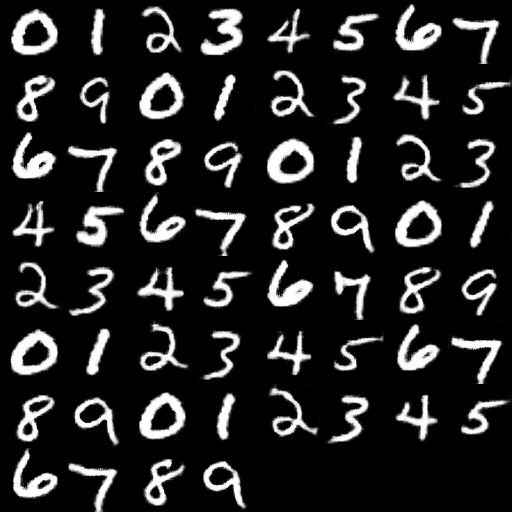
\includegraphics[width=\linewidth]{Bilder/mnist_kedmi.png}
		\caption{Generierung auf Basis eines normalen Modells (MNIST-Generator)}
		\label{img:kedmi_mnist}
	\end{subfigure}
	\hspace{1cm} % Einfügen von horizontalen Abständen zwischen den Bildern
	\begin{subfigure}[b]{0.35\linewidth}
		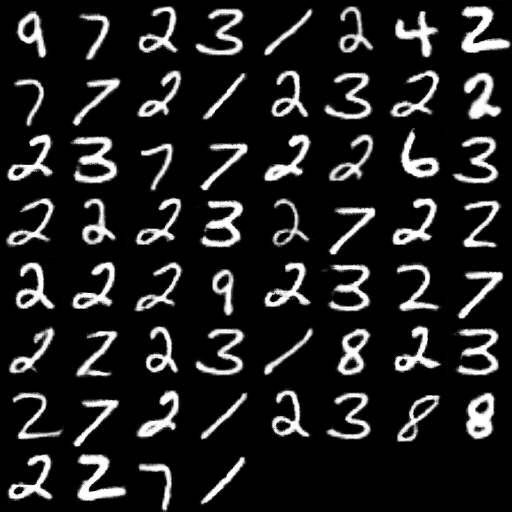
\includegraphics[width=\linewidth]{Bilder/mnist_kedmi_dp.png}
		\caption{Generierung auf Basis eines DP-Modells (MNIST-Generator)}
		\label{img:kedmi_mnist_dp}
	\end{subfigure}
	\begin{subfigure}[b]{\textwidth}
		\centering
		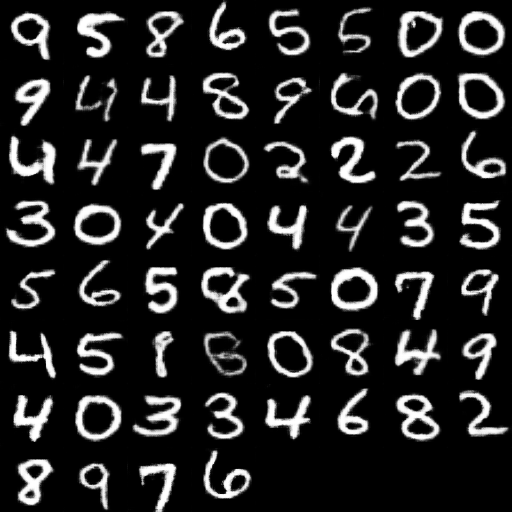
\includegraphics[width=0.35\textwidth]{qmnistdp.png}
		\caption{Generierung auf Basis eines DP-Modells (QMNIST-Generator)}
		\label{img:qmnistdp}
	\end{subfigure}
	\caption{Gegenüberstellung von Rückgenerierungen basierend auf einem normalen Klassifizierer und einem mit differentieller Privatsphäre durch die Ausführung des \glqq KEDMI\grqq-Angriffs}
	\label{img:kedmi_dpvsnorm}
\end{figure}

Im vorliegenden Experiment wurden insgesamt 120 Bilder erzeugt, wobei für jede der zehn Klassen des MNIST-Datensatzes jeweils 6 Bilder verwendet wurden. Die Generierung erfolgte mithilfe einer Modellinversionsattacke, die auf einem herkömmlichen VGG16-Netzwerk basierte. Eine Gruppe von 60 Bildern wurde auf Basis des normalen VGG16-Modells generiert (Beispiel siehe Abbildung \ref{img:kedmi_mnist}), während die restlichen 120 Bilder unter Verwendung eines VGG16-Modells erstellt wurden, das unter Anwendung differenzieller Privatsphäre trainiert wurde (Beispiel siehe Abbildung \ref{img:kedmi_mnist_dp} und \ref{img:qmnistdp}). Die visuelle Analyse dieser umfangreichen Bildersammlung ermöglicht interessante Einblicke in die Wirksamkeit und Robustheit der jeweiligen Modelle.

Die Betrachtung der Bilder, die auf dem konventionellen VGG16-Modell basieren, wie beispielhaft in Abbildung \ref{img:kedmi_mnist} dargestellt, offenbart eine erfolgreiche Generierung für jede der zehn Zielklassen des MNIST-Datensatzes. Die präzisen Darstellungen spiegeln die Intention des Angriffs wider, die einzelnen Ziffern akkurat zu reproduzieren. Dieses Ergebnis unterstreicht die Fähigkeit des Angriffs, aus dem konventionellen Modell die gewünschten Muster und Merkmale adäquat zu rekonstruieren.

Hingegen zeigt die Betrachtung der Bilder, die auf dem VGG16-Modell mit differenzieller Privatsphäre basieren, wie in Abbildung \ref{img:kedmi_mnist_dp} und \ref{img:qmnistdp} exemplarisch dargestellt, auffällige Abweichungen. Die Generierung der Zielklassen weicht zumeist erheblich von der beabsichtigten Darstellung ab, und stattdessen scheinen andere Ziffern in der visuellen Ausgabe präsent zu sein. Diese Unstimmigkeit in der Generierung kann auf die Implementierung differenzieller Privatsphäre zurückgeführt werden, die dem Modell durch ein Rauschen in den Trainingsdaten einen Schutz hinzufügt, um die Vertraulichkeit zu gewährleisten.

Die festgestellte Abweichung zwischen den beiden Gruppen von Bildern belegt, dass die visuelle Repräsentation der Zielklassen durch das Modell mit differenzieller Privatsphäre effektiv verfremdet wurde. Dies lässt darauf schließen, dass die Verteidigungsstrategie in Form der Integration differenzieller Privatsphäre erfolgreich greift. Die Verfälschung der visuellen Ausgabe verhindert, dass sensible Informationen aus den Trainingsdaten extrahiert werden können. Die logische Schlussfolgerung, dass Rückenerierung auf Basis eines \glqq unbekannten Datensatzes\grqq{} bezüglich eines mit differentieller Privatsphäre trainierten Klassifizierers eine ähnliche Ungenauigkeit vorweisen, zeigt Abbildung \ref{img:qmnistdp}.

Eine mögliche Erklärung für die fehlgeschlagene KEDMI-Ausführung auf das Zielmodell mit differenzieller Privatsphäre liegt in der Natur des Angriffs selbst. KEDMI ist ein Whitebox-Angriff, der darauf abzielt, interne Merkmale des Modells zu extrahieren. Da der Angriff bei der differentialen Privatsphäre auf ein Rauschen in den Trainingsdaten stößt, wird die Extraktion genauer Merkmale erschwert. Das Fehlschlagen des Angriffs deutet darauf hin, dass das Modell mit differenzieller Privatsphäre nicht nur einen effektiven Schutz für individuelle Daten bietet, sondern auch erfolgreich gegenüber Whitebox-MI-Angriffen widerstandsfähig ist. Diese Resistenz gegenüber KEDMI legt nahe, dass das Modell ohne Overfitting trainiert wurde und somit keine sensiblen Informationen durch gezielte Angriffe extrahiert werden können.

\begin{figure}[H]
	\centering
	\begin{subfigure}[b]{0.35\linewidth}
		
\includegraphics[width=\linewidth]{Bilder/0_rbmi.png}
		\caption{Generierung der Zahl 0 eines normalen Modells}
		\label{img:rbmi_0}
	\end{subfigure}
	\hspace{1cm} % Einfügen von horizontalen Abständen zwischen den Bildern
	\begin{subfigure}[b]{0.35\linewidth}
		
\includegraphics[width=\linewidth]{Bilder/0_rbmi_dp.png}
		\caption{Generierung der Zahl 0 eines DP-Modells}
		\label{img:rbmi_0_dp}
	\end{subfigure}
	\caption{Gegenüberstellung von Rückgenerierungen der Zahl 0 basierend auf einen normalen Klassifizierer und einem mit differentieller Privatsphäre mit Hilfe des \glqq RBMI\grqq-Angriffs}
	\label{img:rbmi_dpvsnorm}
\end{figure}

In einem weiteren Test wurde die Wirksamkeit der Modelle in Bezug auf eine alternative Modellinversionsattacke, nämlich die RBMI Methode, evaluiert. Hierbei wurden 2 Bilder generiert, wobei die Zielsetzung darin bestand, die Repräsentationsfähigkeit der Modelle unter Verwendung eines anderen Angriffsszenarios zu überprüfen.

Für den ersten Durchlauf erfolgte die Generierung mithilfe der Reinforcement-basierten Modellinversionsattacke auf Grundlage eines herkömmlichen VGG16-Netzwerks. Ein exemplarisches Bild, das die erfolgreiche Generierung der Zahl 0 durch das normale Modell zeigt, ist in Abbildung \ref{img:rbmi_0} dargestellt. Die visuelle Analyse verdeutlicht, dass das herkömmliche Modell auch unter diesem alternativen Angriffsszenario in der Lage ist, die Zielklasse präzise zu reproduzieren.

Im Gegensatz dazu erfolgte die Generierung des zweiten Bildes unter Anwendung der Reinforcement-basierten Modellinversionsattacke auf einem VGG16-Modell, das mit differenzieller Privatsphäre trainiert wurde. Ein repräsentatives Bild dieses Sets, das die Zahl 0 durch das differenziell private Modell darstellen soll, ist in Abbildung \ref{img:rbmi_0_dp} zu sehen. Bei der visuellen Analyse fällt auf, dass im Gegensatz zum normalen Modell die Generierung durch das differenziell private Modell fehlschlägt, und die Zahl 0 nicht erkennbar ist. Stattdessen lässt sich die Zahl 4 erkennen.

Die festgestellten Unterschiede in der Generierung zwischen den beiden Modellen bei Anwendung der Reinforcement-basierten Modellinversionsattacke legen nahe, dass das Modell mit differenzieller Privatsphäre auch unter dieser alternativen Bedrohung effektive Schutzmechanismen aufweist. Während das herkömmliche Modell weiterhin die gewünschten Muster präzise reproduziert, bleibt das differenzielle Modell widerstandsfähig gegenüber dem Angriff und verhindert die korrekte Rekonstruktion der Zielklasse. Dies untermauert die Robustheit der differenziellen Privatsphäre als Verteidigungsstrategie, selbst unter unterschiedlichen Angriffsszenarien.

Die visuelle Analyse der Verteidigungsstrategie \glqq Differential Privacy\grqq{} demonstriert eine erfolgreiche Verfremdung der Generierungen durch ein Modell mit differenzieller Privatsphäre im Vergleich zu einem herkömmlichen Modell. Bei der Anwendung von Modellinversionsattacken wie dem \glqq KEDMI\grqq- und \glqq RBMI\grqq-Angriff zeigt sich eine deutliche Unkenntlichmachung der Zielklassen. Dies verdeutlicht die Effektivität von Differential Privacy im Schutz sensibler Informationen in den visuellen Repräsentationen.

Die festgestellten Unterschiede in der Generierung zwischen den Modellen deuten darauf hin, dass das Modell mit differenzieller Privatsphäre auch unter unterschiedlichen Angriffsszenarien robust agiert. Die visuelle Unkenntlichmachung der Zielklassen kann als positiver Effekt gewertet werden, da sie darauf hinweist, dass Differential Privacy sensible Informationen effektiv schützt. Der Schwerpunkt auf der visuellen Analyse liefert einen klaren Einblick in die Wirksamkeit der Verteidigungsstrategie.

Die visuelle Auswertung bildet jedoch nur einen Teil der umfassenden Analyse. Der statistische Teil wird nun genauer betrachtet, wobei quantitative Metriken und qualitative Aspekte berücksichtigt werden. Dies ermöglicht eine detailliertere Bewertung der Wirksamkeit von Differential Privacy und dessen Auswirkungen auf die Präzision von Angriffen und Klassifikationen.

\begin{table}[h]
	\centering
	\renewcommand{\arraystretch}{1.5}
	\resizebox{\textwidth}{!}{
		\begin{tabular}{|c|c|c|c|c|c|}
			\hline
		\textbf{Zielmodell} & \textbf{Angriffsart} & \textbf{Datensatz} & \textbf{Iterationen} & \textbf{Gesamtdauer} & \textbf{Genauigkeit}\\
			\hline
			\textit{VGG16} & KEDMI & MNIST & 2.400 & 4 min & \textbf{100,0\%}\\
			\hline
  			\textit{DP-VGG16} & KEDMI & MNIST & 2.400 & 4 min 30 sec & \textbf{13,33\%}\\
			\hline
			\textit{VGG16} & RBMI & MNIST & 40.000 & 12 min & \textbf{100,0\%}\\
			\hline
		    \textit{DP-VGG16} & RBMI & MNIST & 40.000 & 11 min 24 sec & \textbf{10,17\%}\\
			\hline
		\end{tabular}
	}
	\caption{Auswertung zweier Angriffsalgorithmen auf \glqq abgesicherte\grqq{} und ungeschützte Modelle}
	\label{tab:dp_stats}
\end{table}

Die Analyse der Ergebnisse in Tabelle \ref{tab:dp_stats} offenbart eine deutliche Abnahme der Genauigkeit von Modell-Inversionsangriffen bei einem Modell, das mit differenzieller Privatsphäre trainiert wurde. Diese Abnahme der Genauigkeit lässt sich als Indikator interpretieren, dass die generierten Bilder größtenteils nicht korrekt der Zielklasse zugeordnet werden können und somit die Wirksamkeit der differenziellen Privatsphäre in der Abwehr von Modell-Inversionsangriffen verdeutlicht wird.

Die Integration von Rauschen in die Trainingsdaten hat sich als effektive Verteidigungsstrategie erwiesen, da die extrahierte Merkmalsrepräsentation für Modell-Inversionsangriffe erschwert wird. Die generierten Repräsentationen weisen häufiger falsche Klassifikationen auf, was darauf hindeutet, dass die Zielklassen nur unzureichend reproduziert werden können. Dies bestätigt die Schutzwirkung von Differential Privacy in Bezug auf die Verhinderung präziser Rekonstruktionen durch Modell-Inversionsangriffe.

Die Dauer pro Iteration des Angriffs zeigt nur minimale Unterschiede zwischen einem normalen Modell und einem Modell mit differenzieller Privatsphäre. Dies lässt sich auf den unveränderten Generator und den gleichen Algorithmus des Angriffs zurückführen. Die vergleichbare Zeitdauer verdeutlicht, dass trotz der erschwerten Generierung durch Differential Privacy, die Effizienz des Angriffsprozesses nur geringfügig beeinflusst wird.

Interessanterweise weisen verschiedene Arten von Modell-Inversionsangriffen, darunter Black- und Whitebox-Angriffe, keine signifikanten Unterschiede in der Genauigkeit auf. Dies legt nahe, dass die Verteidigungsmechanismen von Differential Privacy robust gegenüber unterschiedlichen Angriffsarten sind. Selbst bei Kenntnis der internen Struktur des Modells (Whitebox) oder im Falle fehlender interner Informationen (Blackbox) zeigt die differenzielle Privatsphäre eine gleichbleibende Schutzwirkung. Diese Homogenität in der Abwehrleistung unterstreicht die Vielseitigkeit von Differential Privacy als Verteidigungsstrategie gegenüber Modell-Inversionsangriffen.


   \chapter{Zusammenfassung und Ausblick} \label{chpt:Zusammenfassung_und_Ausblick_Main}



   \chapter{Anhang} \label{chpt:Anhang_Main}


Hier sind noch \LaTeX-Beispiele für die Verwendung: 

...
\newline
\newline
Tabelle erzeugen: 
\begin{table}[htbp]
	\centering
	\caption{Beispieltabelle}
	\begin{tabularx}{\textwidth}{|X|X|X|X|}
		\hline
		Spalte 1 & Spalte 2 & Spalte 3 & Spalte 4 \\
		\hline
		Inhalt 1 & Inhalt 2 & Inhalt 3 & Inhalt 4 \\
		\hline
		Inhalt 5 & Inhalt 6 & Inhalt 7 & Inhalt 8 \\
		\hline
	\end{tabularx}
\end{table}

...
\newline
\newline
Quellen verlinken: 
% Quellenverlinkung
Test \cite{Bar-Shalom}.
Test \cite{Goldhammer}.
Test \cite{WHO-2004}.

...
\newline
\newline
Kapitel verlinken: 
% Kapitelverlinkung
Wie in Abschnitt \ref{chpt:Ergebnisse_Main} beschrieben wird ...

...
\newline
\newline
% Einfügen einer Grafik/Bildes etc.
\begin{figure}[ht]
	\centering
	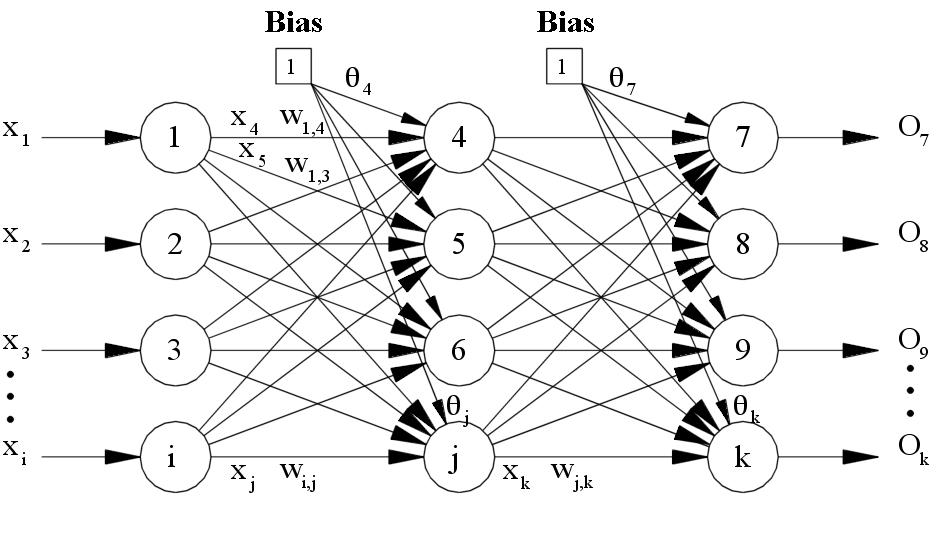
\includegraphics[scale=0.40]{Bilder/Neural_Network.jpg}
	\caption{Beispielbild}
	\label{fig: Neural_Network_Fig}
\end{figure}




   
       
   %%%%%%%%%%%%%%%%%%%%%%%%%%%%%%%%%%%%%%%%%%%%%%%%%%%%%%%%%%%%%%
   
   % Weitere Verzeichnisse
   
   \listoffigures          							% Abbildungsverzeichnis
   \listoftables           							% Tabellenverzeichnis
   %   \lstlistoflistings      						% Codeverzeichnis   
   
   %   \setbibpreamble{Prambel}    					% Text vor dem Verzeichnis
   %   \nocite{*}									% Falls eine nicht-zitierte Quelle im PDF erscheinen soll
   %   \bibliographystyle{dinat}
   %   \begin{flushleft}
   % \begin{small} 
   % Bibliographie Style - dinat muss installiert sein
   %   \bibliography{Kapitel/Literatur}					% Bibliographie erzeugen
   %\end{small} 
   %	\end{flushleft}	
  ( \cite{lorenz_reinforcement_2020})
   
   %\nocite{*}
  \printbibheading
  \printbibliography[heading=subbibliography,type=book,title={B{\"u}cher}]
  \newpage
  \printbibliography[heading=subbibliography, type=collection, title={Sammlungen}]
  \newpage
  \printbibliography[heading=subbibliography,type=article,title={Artikel}]
  \printbibliography[heading=subbibliography,type=inproceedings,title={Konferenzbeiträge}]
  
   
   
   
   %\printbibliography	
		
%   \includepdfset{pagecommand={\thispagestyle{headings}}}
%   \automark[section]{section}
%   \lhead{Abkuerzungen}
   
   %\refstepcounter{chapter}
   %\chaptermark{Abkürzungen}
   %%%%%%%%%%%%%%%%%%%%%%%%%%%%%%%%%%%%%%%%%%%%%%%%%%%%%%%%%%%%%%%
\renewcommand*{\acsfont}[1]{\normalfont{\normalsize{#1}}}

\chapter*{Abkürzungen}
\addcontentsline{toc}{chapter}{Abkürzungen}

\begin{acronym}[Abkürzungen]
   % Numerische Abkürzungen
   
   % 'A' 
   \acro{ML}     		{\textit{Maschinelles Lernen}}
   % 'B' 
   
   % 'C' 
   \acro{CNN}{\textit{Convolutional Neural Network}}
   
   % 'D' 
   \acro{DCGAN}{\textit{Deep Convolutional Generative Adversarial Network}}
   \acro{DP}{\textit{differentielle Privatsphäre, eng.: Differential Privacy}}

   % 'E' 
   
   % 'F' 

   % 'G'

   % 'H' 
       
   % 'I'
   
   % 'J' 
   
   % 'K' 
   \acro{KEDMI}{\textit{Knowledge-Enriched-Distributional Model Inversion}}
   \acro{KNN}{\textit{Künstlich-Neuronales Netzwerk}}
   
   % 'L' 
   
   % 'M' 

   % 'N' 
   \acro{NN}{\textit{Neuronales Netzwerk, eng.: Neural Network}}
     
   % 'O'  
   
   % 'P'  

   % 'Q' 
   
   % 'R' 
   \acro{RBMI}{\textit{Reinforcement-Based Model Inverion}}
		
   % 'S' 

   % 'T' 
   
   % 'U' 
   
   % 'V' 
   
   % 'W' 
   
   % 'X', 'Y', 'Z' 

\end{acronym}							% Abkürzungsverzeichnis						   

   
\end{document}
%%%%%%%%%%%%%%%%%%%%%%%%%%%%%%%%%%%%%%%%%%%%%%%%%%%%%%%%%%%%%%%%%%%%%%%
%%%                           Dokumentende                          %%%
%%%%%%%%%%%%%%%%%%%%%%%%%%%%%%%%%%%%%%%%%%%%%%%%%%%%%%%%%%%%%%%%%%%%%%%
